% -*- Mode:TeX -*-

%% IMPORTANT: The official thesis specifications are available at:
%%            http://libraries.mit.edu/archives/thesis-specs/
%%
%%            Please verify your thesis' formatting and copyright
%%            assignment before submission. If you notice any
%%            discrepancies between these templates and the 
%%            MIT Libraries' specs, please let us know
%%            by e-mailing thesis@mit.edu

%% The documentclass options along with the pagestyle can be used to generate
%% a technical report, a draft copy, or a regular thesis. You may need to
%% re-specify the pagestyle after you \include cover.tex. For more
%% information, see the first few lines of mitthesis.cls. 

%\documentclass[12pt,vi,twoside]{mitthesis}
%%
%%  If you want your thesis copyright to you instead of MIT, use the
%%  ``vi'' option, as above.
%%
%\documentclass[12pt,twoside,leftblank]{mitthesis}
%%
%% If you want blank pages before new chapters to be labelled ``This
%% Page Intentionally Left Blank'', use the ``leftblank'' option, as
%% above. 

\documentclass[12pt,twoside]{mitthesis}
\usepackage{lgrind}

\usepackage{amsmath}
\usepackage{amssymb}
\usepackage{algorithm}
\usepackage{algpseudocode}
\usepackage{enumitem}
\usepackage{titlesec}
\usepackage{mathtools}



\titlespacing*{\chapter}
{5pt}{5pt}{5pt}
\titlespacing*{\section}
{5pt}{5pt}{5pt}
\titlespacing*{\subsection}
{5pt}{5pt}{5pt}
\titlespacing*{\subsubsection}
{5pt}{5pt}{5pt}
\titlespacing*{\paragraph}
{5pt}{5pt}{5pt}

\setitemize{noitemsep,topsep=0pt,parsep=0pt,partopsep=0pt}
\setenumerate{noitemsep,topsep=0pt,parsep=0pt,partopsep=0pt}

\setlength{\parindent}{4em}
\setlength{\parskip}{1em}

\DeclarePairedDelimiter\abs{\lvert}{\rvert}
\DeclarePairedDelimiter\norm{\lVert}{\rVert}

% \newcommand\norm[1]{\left\lVert#1\right\rVert}

%% These have been added at the request of the MIT Libraries, because
%% some PDF conversions mess up the ligatures.  -LB, 1/22/2014
\usepackage{cmap}
\usepackage[T1]{fontenc}
\usepackage{graphicx}
\graphicspath{ {./figures/} }
\pagestyle{plain}

%% This bit allows you to either specify only the files which you wish to
%% process, or `all' to process all files which you \include.
%% Krishna Sethuraman (1990).

%\typein [\files]{Enter file names to process, (chap1,chap2 ...), or `all' to process all files:}
\def\all{all}
\ifx\files\all \typeout{Including all files.} \else %\typeout{Including only \files.} \includeonly{\files} \fi

\begin{document}

% -*-latex-*-
% 
% For questions, comments, concerns or complaints:
% thesis@mit.edu
% 
%
% $Log: cover.tex,v $
% Revision 1.9  2019/08/06 14:18:15  cmalin
% Replaced sample content with non-specific text.
%
% Revision 1.8  2008/05/13 15:02:15  jdreed
% Degree month is June, not May.  Added note about prevdegrees.
% Arthur Smith's title updated
%
% Revision 1.7  2001/02/08 18:53:16  boojum
% changed some \newpages to \cleardoublepages
%
% Revision 1.6  1999/10/21 14:49:31  boojum
% changed comment referring to documentstyle
%
% Revision 1.5  1999/10/21 14:39:04  boojum
% *** empty log message ***
%
% Revision 1.4  1997/04/18  17:54:10  othomas
% added page numbers on abstract and cover, and made 1 abstract
% page the default rather than 2.  (anne hunter tells me this
% is the new institute standard.)
%
% Revision 1.4  1997/04/18  17:54:10  othomas
% added page numbers on abstract and cover, and made 1 abstract
% page the default rather than 2.  (anne hunter tells me this
% is the new institute standard.)
%
% Revision 1.3  93/05/17  17:06:29  starflt
% Added acknowledgements section (suggested by tompalka)
% 
% Revision 1.2  92/04/22  13:13:13  epeisach
% Fixes for 1991 course 6 requirements
% Phrase "and to grant others the right to do so" has been added to 
% permission clause
% Second copy of abstract is not counted as separate pages so numbering works
% out
% 
% Revision 1.1  92/04/22  13:08:20  epeisach

% NOTE:
% These templates make an effort to conform to the MIT Thesis specifications,
% however the specifications can change. We recommend that you verify the
% layout of your title page with your thesis advisor and/or the MIT 
% Libraries before printing your final copy.
\title{Smooth and Interactive Parametrization-Based Quadrangulation}

\author{Roy Velich}
% If you wish to list your previous degrees on the cover page, use the 
% previous degrees command:
%       \prevdegrees{A.A., Harvard University (1985)}
% You can use the \\ command to list multiple previous degrees
%       \prevdegrees{B.S., University of California (1978) \\
%                    S.M., Massachusetts Institute of Technology (1981)}
\department{Department of Computer Science}

% If the thesis is for two degrees simultaneously, list them both
% separated by \and like this:
% \degree{Doctor of Philosophy \and Master of Science}
\degree{Master of Science in Computer Science}

% As of the 2007-08 academic year, valid degree months are September, 
% February, or June.  The default is June.
\degreemonth{November}
\degreeyear{2020}
\thesisdate{November 30, 2020}

%% By default, the thesis will be copyrighted to MIT.  If you need to copyright
%% the thesis to yourself, just specify the `vi' documentclass option.  If for
%% some reason you want to exactly specify the copyright notice text, you can
%% use the \copyrightnoticetext command.  
%\copyrightnoticetext{\copyright IBM, 1990.  Do not open till Xmas.}

% If there is more than one supervisor, use the \supervisor command
% once for each.
\supervisor{Dr. Roi Poranne}{Assistant Professor}

% This is the department committee chairman, not the thesis committee
% chairman.  You should replace this with your Department's Committee
% Chairman.
\chairman{Prof. Ronen Shaltiel}{Chairman, Department Committee on Graduate Theses}

% Make the titlepage based on the above information.  If you need
% something special and can't use the standard form, you can specify
% the exact text of the titlepage yourself.  Put it in a titlepage
% environment and leave blank lines where you want vertical space.
% The spaces will be adjusted to fill the entire page.  The dotted
% lines for the signatures are made with the \signature command.
\maketitle

% The abstractpage environment sets up everything on the page except
% the text itself.  The title and other header material are put at the
% top of the page, and the supervisors are listed at the bottom.  A
% new page is begun both before and after.  Of course, an abstract may
% be more than one page itself.  If you need more control over the
% format of the page, you can use the abstract environment, which puts
% the word "Abstract" at the beginning and single spaces its text.

%% You can either \input (*not* \include) your abstract file, or you can put
%% the text of the abstract directly between the \begin{abstractpage} and
%% \end{abstractpage} commands.

% First copy: start a new page, and save the page number.
\cleardoublepage
% Uncomment the next line if you do NOT want a page number on your
% abstract and acknowledgments pages.
% \pagestyle{empty}
\setcounter{savepage}{\thepage}
\begin{abstractpage}
% $Log: abstract.tex,v $
% Revision 1.1  93/05/14  14:56:25  starflt
% Initial revision
% 
% Revision 1.1  90/05/04  10:41:01  lwvanels
% Initial revision
% 
%
%% The text of your abstract and nothing else (other than comments) goes here.
%% It will be single-spaced and the rest of the text that is supposed to go on
%% the abstract page will be generated by the abstractpage environment.  This
%% file should be \input (not \include 'd) from cover.tex.
\begin{figure}[ht]
\centering
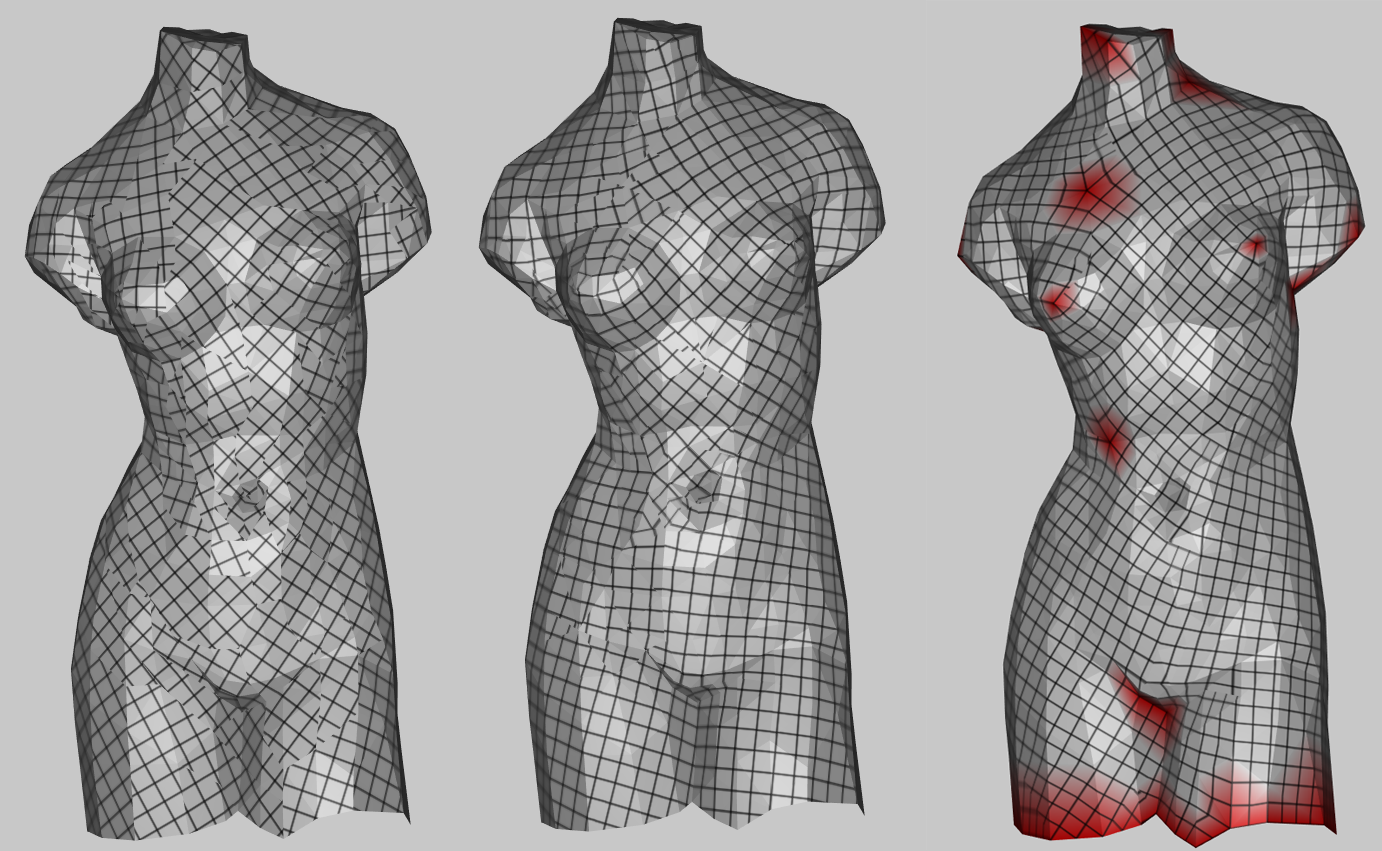
\includegraphics[width=15cm]{figures/teaser.png}
\caption[Abstract's Teaser]{\textbf{Left:} Initial mapping of cut mesh. {Middle:} With increased penalty on seamlessness violation. {Right:} With increased penalty on integer violation.}
\label{fig:teaser}
\end{figure}

\subsubsection{Introduction}
Many applications in computer graphics, such as character modeling and animation, architectural geometry, and also physical simulation to some extent, call for quad meshes as a representation of the geometry \cite{10.1111/cgf.12014}. However, since triangle meshes are generally more prevalent, they need to be convert via the process known as \emph{quad remeshing}.

\noindent Numerous techniques were introduced in recent years, and the most common approach is to split the problem into cross field generation, and field guided parameterization. In this document, we present an interactive, direct parametrization approach, which nullifies the need for intermediate steps.

\noindent The idea behind parameterization based methods in general, is to map the mesh to the plane, and create a regular grid layout on it. In order to ensure that the grid on the plane is transformed into a valid quad mesh on the surface, certain conditions on the parameterization must be fulfilled \cite{bommes:hal-00862648}:

\begin{enumerate}
  \item \textbf{Seamless Condition}: The transition function $g_{ij}$ between two half-edges $e_i$ and $e_j$ on the parameterization domain that corresponds to the same surface edge that is part of a cut seam, has to be an integer-grid automorphism given by:
  $$e_j = R^{r_{ij}}_{90^\circ}e_i + \vec{t}_{ij}$$
  Where  $r_{ij} \in \{0,1,2,3\}$ and $\vec{t}_{ij} \in \mathbb{Z}^2$.
  
  \item \textbf{Singular-Points Condition}: All singular vertices, which are characterized by a non-zero angular defect on the parameterization domain, have to lie on integer locations. That is, given the set $S_i$ of all parameterization domain vertices that correspond to the same singular surface vertex $v_i$, we require that:
  $$\forall u \in S_i: u \in \mathbb{Z}^2 $$
  
  \item \textbf{Consistent Orientation Condition}: All triangles on the parameterization domain should have the same orientation. That is, we should not allow triangle flips after initial mapping is formed.
\end{enumerate}

\subsubsection{Our Approach}
Inspired by \cite{Poranne:Autocuts:2017}, we employ a direct approach to the problem of quadrangulating a triangle mesh, by formulating and solving a smooth optimization problem. We model smooth penalty functions for the first two conditions mentioned above (Seamless and Singular-Points), and add to it an additional penalty, the Symmetric Dirichlet energy, which prevents triangle flips and penalize triangle distortion.
Since all of our penalty functions are smooth, we can analytically derive their gradients and hessians, and utilize Newton's method to iteratively solve for a mapping that renders a valid quad mesh on the 3D surface.

\noindent Our smooth approach allows us to visualize the whole optimization process for the end-user as an interactive design tool, which empowers the user to guide the algorithm to the desired result by gradually changing penalty weights, grid resolution, guiding quads direction using brush tool, and more. The user receives immediate feedback for any change applied to the problem settings. Figure \ref{fig:teaser} illustrates the three main stages of our approach. First, the 3D surface is cut into the plane. Then, the seamless penalty function weight gradually increased. Finally, the singular points penalty function is turned on to place singular vertices at integer locations.

\subsubsection{Details}
\paragraph{Initialization}
We cut the mesh by mapping its dual spanning tree to the parameterization plane isometrically as a triangle soup. We first map an arbitrary initial triangle to the parameterization plane. Then, we map to the plane all neighbour triangles of the initial triangle, such that adjacent triangles share an edge. We continue this process for the next layer of neighbours, till we map all of the mesh's triangles.
\subsubsection{Seamless Penalty Functions}
\paragraph{Angle Penalty}
Given two half-edges $e_i$ and $e_j$ on the parameterization domain that corresponds to the same surface edge, we penalize the angle between them as follows: 
$$P_{\mathrm{angle}}\left(e_i,e_j\right) = \sin\left(4\left(\theta(e_i) - \theta(e_j) \right) - \frac{\pi}{2} \right) + 1$$
Where $\theta(e_i)$ and $\theta(e_j)$ are the angles of the two half edges $e_i$ and $e_j$, respectively. For any $k \in \mathbb{Z}$ such that $\theta(e_i) - \theta(e_j) = \frac{\pi}{2}k$ we have that $P_{\mathrm{angle}}\left(e_i,e_j\right) = 0$. Therefore, $P_{\mathrm{angle}}$ will penalize half-edges of which their angle discrepancy differs from a multiple of $90^\circ$.
\paragraph{Length Penalty}
We penalize the length discrepancy between the two half-edges with the following penalty function:
$$P_{\mathrm{length}}\left(e_i,e_j\right) = \left( \norm{e_i}^2 - \norm{e_j}^2 \right)^2$$
Only when the two half-edges have the same length, we have that $P_{\mathrm{length}}\left(e_i,e_j\right) = 0$.
\paragraph{Translation Penalty}
We penalize for non-integer translation between the two half-edges as follows:
\begin{multline}
P_{\mathrm{translation}}\left(e_i,e_j\right) = \sin\left(2\pi\left(x_{e_i} - x_{e_j}\right) - \frac{\pi}{2} \right) + 1 \\ + \sin\left(2\pi\left(y_{e_i} - y_{e_j}\right) - \frac{\pi}{2} \right) + 1 \nonumber
\end{multline}
Where $\left(x_{e_i}, y_{e_i}\right)$ and $\left(x_{e_j}, y_{e_j}\right)$ are the coordinates of two corresponding vertices of the two half-edges $e_i$ and $e_j$.
\subsubsection{Singular-Points Penalty Function}
To satisfy the singularity points condition, all vertices on the parameterization domain which correspond to the same vertex on the surface, have to lie on integer locations if they are characterized by a non-zero angle defect in the domain. Therefore, we penalize singular points as follows:
\begin{multline}
P_{\mathrm{singularity}}\left(S\right) = \sum_{u \in S} \left( \sin\left(2 \pi x_{u} - \frac{\pi}{2} \right) + 1 + \sin\left(2 \pi y_{u} - \frac{\pi}{2} \right) + 1 \right) \nonumber
\end{multline}
Where $S$ is a set of domain vertices with non-zero angle defect, which correspond to the same surface vertex, and $\left(x_u,y_u\right)$ are the coordinates of the domain vertex $u \in S$. We weight $P_{\mathrm{singularity}}$ by the magnitude of the angle defect.
\subsubsection{Consistent Orientation and Distortion Penalty Functions}
To satisfy the consistent orientation condition, and to minimize triangle distortion, we use the symmetric dirichlet energy \cite{10.1145/2766947}, which prevents triangle flips. The symmetric dirichlet penalty function is given as follows:
$$
P_{\mathrm{dirichlet}}\left(t_i\right) = \norm{J\left(t_i\right)}_F^2 + \norm{J^{-1}\left(t_i\right)}_F^2 \nonumber
$$
Where $J\left(t_i\right)$ is the Jacobian of the mapping of triangle $t_i$ and $\norm{\cdot}_F$ is the Frobenius norm.
\subsubsection{Optimization Process}
In order to find a parameterization which forms a valid quad mesh on the 3D surface, we solve the following unconstrained optimization problem:
\begin{alignat}{2}
  &\min_{X}
     &\quad & \sum_{i \sim j} P_{\mathrm{angle}}\left(e_i,e_j\right) + P_{\mathrm{length}}\left(e_i,e_j\right) + P_{\mathrm{translation}}\left(e_i,e_j\right) \nonumber\\ 
  &  &  & + \sum_{i} P_{\mathrm{singularity}}\left(S_i\right) \nonumber\\ 
  &  &  & + \sum_{i} P_{\mathrm{dirichlet}}\left(t_i\right) \nonumber
\end{alignat}
Where $X$ denotes the set of variables of the optimization problem, i.e., the coordinates of the vertices in the parameterization domain. We derive the analytical expressions for the gradient and Hessian of each penalty function and make sure that all Hessians are positive semi-definite by zeroing negative eigenvalues. We solve the optimization problem using Newton's method. In iteration $n$, we evaluate the gradient $g^{(n)}$ and Hessian $H^{(n)}$ of our total objective function at $X^{(n)}$, and solve the Newton equation $H^{(n)}p^{(n)}=-g^{(n)}$ which yields a search direction $p^{(n)}$. The next iterate is obtained by $X^{(n+1)} = X^{(n)} + \alpha p^{(n)}$ where the optimal $\alpha$ is found using line search. We use Intel's Pardiso solver to solve the sparse Newton equation.

\end{abstractpage}

% Additional copy: start a new page, and reset the page number.  This way,
% the second copy of the abstract is not counted as separate pages.
% Uncomment the next 6 lines if you need two copies of the abstract
% page.
% \setcounter{page}{\thesavepage}
% \begin{abstractpage}
% % $Log: abstract.tex,v $
% Revision 1.1  93/05/14  14:56:25  starflt
% Initial revision
% 
% Revision 1.1  90/05/04  10:41:01  lwvanels
% Initial revision
% 
%
%% The text of your abstract and nothing else (other than comments) goes here.
%% It will be single-spaced and the rest of the text that is supposed to go on
%% the abstract page will be generated by the abstractpage environment.  This
%% file should be \input (not \include 'd) from cover.tex.
\begin{figure}[ht]
\centering
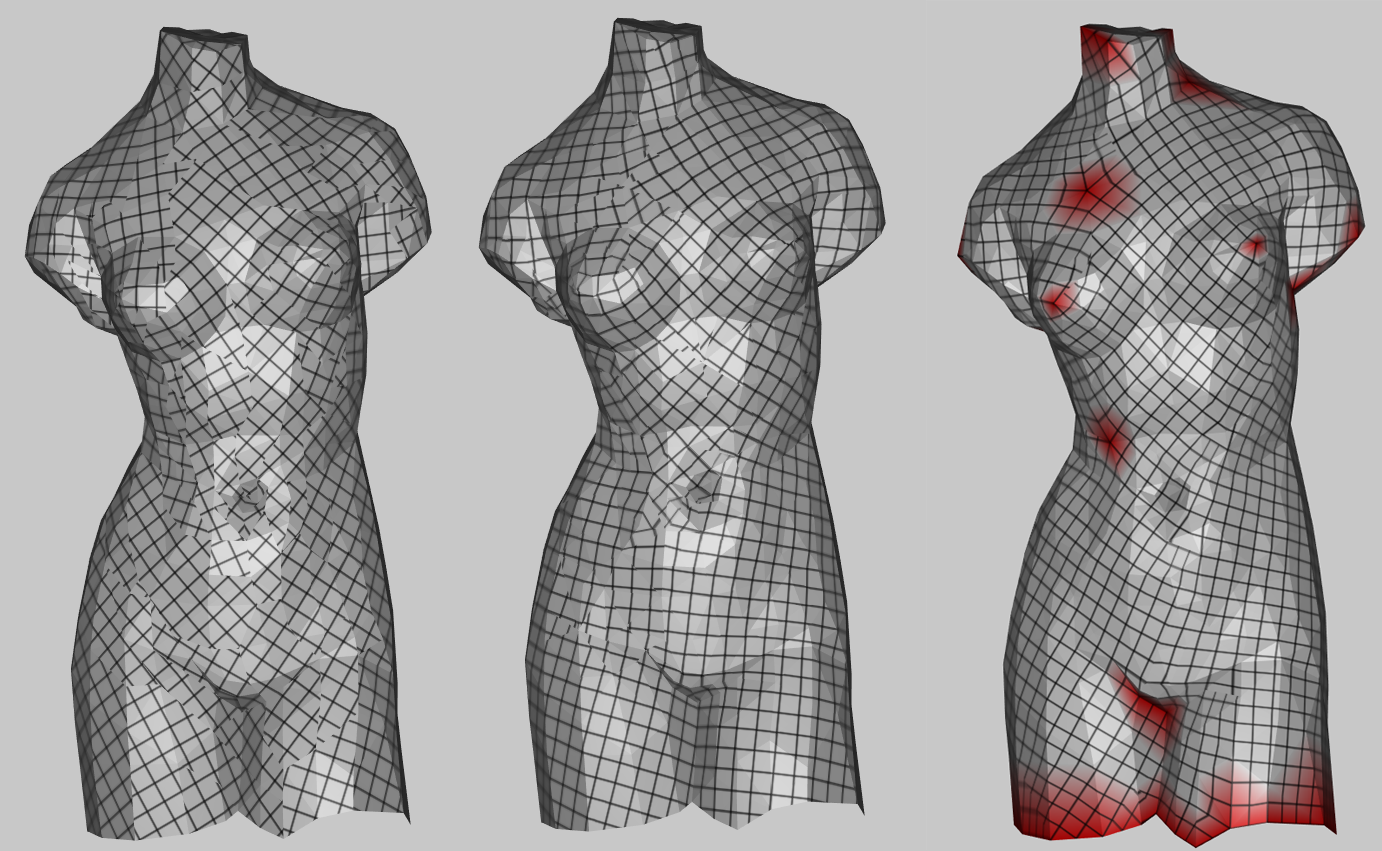
\includegraphics[width=15cm]{figures/teaser.png}
\caption[Abstract's Teaser]{\textbf{Left:} Initial mapping of cut mesh. {Middle:} With increased penalty on seamlessness violation. {Right:} With increased penalty on integer violation.}
\label{fig:teaser}
\end{figure}

\subsubsection{Introduction}
Many applications in computer graphics, such as character modeling and animation, architectural geometry, and also physical simulation to some extent, call for quad meshes as a representation of the geometry \cite{10.1111/cgf.12014}. However, since triangle meshes are generally more prevalent, they need to be convert via the process known as \emph{quad remeshing}.

\noindent Numerous techniques were introduced in recent years, and the most common approach is to split the problem into cross field generation, and field guided parameterization. In this document, we present an interactive, direct parametrization approach, which nullifies the need for intermediate steps.

\noindent The idea behind parameterization based methods in general, is to map the mesh to the plane, and create a regular grid layout on it. In order to ensure that the grid on the plane is transformed into a valid quad mesh on the surface, certain conditions on the parameterization must be fulfilled \cite{bommes:hal-00862648}:

\begin{enumerate}
  \item \textbf{Seamless Condition}: The transition function $g_{ij}$ between two half-edges $e_i$ and $e_j$ on the parameterization domain that corresponds to the same surface edge that is part of a cut seam, has to be an integer-grid automorphism given by:
  $$e_j = R^{r_{ij}}_{90^\circ}e_i + \vec{t}_{ij}$$
  Where  $r_{ij} \in \{0,1,2,3\}$ and $\vec{t}_{ij} \in \mathbb{Z}^2$.
  
  \item \textbf{Singular-Points Condition}: All singular vertices, which are characterized by a non-zero angular defect on the parameterization domain, have to lie on integer locations. That is, given the set $S_i$ of all parameterization domain vertices that correspond to the same singular surface vertex $v_i$, we require that:
  $$\forall u \in S_i: u \in \mathbb{Z}^2 $$
  
  \item \textbf{Consistent Orientation Condition}: All triangles on the parameterization domain should have the same orientation. That is, we should not allow triangle flips after initial mapping is formed.
\end{enumerate}

\subsubsection{Our Approach}
Inspired by \cite{Poranne:Autocuts:2017}, we employ a direct approach to the problem of quadrangulating a triangle mesh, by formulating and solving a smooth optimization problem. We model smooth penalty functions for the first two conditions mentioned above (Seamless and Singular-Points), and add to it an additional penalty, the Symmetric Dirichlet energy, which prevents triangle flips and penalize triangle distortion.
Since all of our penalty functions are smooth, we can analytically derive their gradients and hessians, and utilize Newton's method to iteratively solve for a mapping that renders a valid quad mesh on the 3D surface.

\noindent Our smooth approach allows us to visualize the whole optimization process for the end-user as an interactive design tool, which empowers the user to guide the algorithm to the desired result by gradually changing penalty weights, grid resolution, guiding quads direction using brush tool, and more. The user receives immediate feedback for any change applied to the problem settings. Figure \ref{fig:teaser} illustrates the three main stages of our approach. First, the 3D surface is cut into the plane. Then, the seamless penalty function weight gradually increased. Finally, the singular points penalty function is turned on to place singular vertices at integer locations.

\subsubsection{Details}
\paragraph{Initialization}
We cut the mesh by mapping its dual spanning tree to the parameterization plane isometrically as a triangle soup. We first map an arbitrary initial triangle to the parameterization plane. Then, we map to the plane all neighbour triangles of the initial triangle, such that adjacent triangles share an edge. We continue this process for the next layer of neighbours, till we map all of the mesh's triangles.
\subsubsection{Seamless Penalty Functions}
\paragraph{Angle Penalty}
Given two half-edges $e_i$ and $e_j$ on the parameterization domain that corresponds to the same surface edge, we penalize the angle between them as follows: 
$$P_{\mathrm{angle}}\left(e_i,e_j\right) = \sin\left(4\left(\theta(e_i) - \theta(e_j) \right) - \frac{\pi}{2} \right) + 1$$
Where $\theta(e_i)$ and $\theta(e_j)$ are the angles of the two half edges $e_i$ and $e_j$, respectively. For any $k \in \mathbb{Z}$ such that $\theta(e_i) - \theta(e_j) = \frac{\pi}{2}k$ we have that $P_{\mathrm{angle}}\left(e_i,e_j\right) = 0$. Therefore, $P_{\mathrm{angle}}$ will penalize half-edges of which their angle discrepancy differs from a multiple of $90^\circ$.
\paragraph{Length Penalty}
We penalize the length discrepancy between the two half-edges with the following penalty function:
$$P_{\mathrm{length}}\left(e_i,e_j\right) = \left( \norm{e_i}^2 - \norm{e_j}^2 \right)^2$$
Only when the two half-edges have the same length, we have that $P_{\mathrm{length}}\left(e_i,e_j\right) = 0$.
\paragraph{Translation Penalty}
We penalize for non-integer translation between the two half-edges as follows:
\begin{multline}
P_{\mathrm{translation}}\left(e_i,e_j\right) = \sin\left(2\pi\left(x_{e_i} - x_{e_j}\right) - \frac{\pi}{2} \right) + 1 \\ + \sin\left(2\pi\left(y_{e_i} - y_{e_j}\right) - \frac{\pi}{2} \right) + 1 \nonumber
\end{multline}
Where $\left(x_{e_i}, y_{e_i}\right)$ and $\left(x_{e_j}, y_{e_j}\right)$ are the coordinates of two corresponding vertices of the two half-edges $e_i$ and $e_j$.
\subsubsection{Singular-Points Penalty Function}
To satisfy the singularity points condition, all vertices on the parameterization domain which correspond to the same vertex on the surface, have to lie on integer locations if they are characterized by a non-zero angle defect in the domain. Therefore, we penalize singular points as follows:
\begin{multline}
P_{\mathrm{singularity}}\left(S\right) = \sum_{u \in S} \left( \sin\left(2 \pi x_{u} - \frac{\pi}{2} \right) + 1 + \sin\left(2 \pi y_{u} - \frac{\pi}{2} \right) + 1 \right) \nonumber
\end{multline}
Where $S$ is a set of domain vertices with non-zero angle defect, which correspond to the same surface vertex, and $\left(x_u,y_u\right)$ are the coordinates of the domain vertex $u \in S$. We weight $P_{\mathrm{singularity}}$ by the magnitude of the angle defect.
\subsubsection{Consistent Orientation and Distortion Penalty Functions}
To satisfy the consistent orientation condition, and to minimize triangle distortion, we use the symmetric dirichlet energy \cite{10.1145/2766947}, which prevents triangle flips. The symmetric dirichlet penalty function is given as follows:
$$
P_{\mathrm{dirichlet}}\left(t_i\right) = \norm{J\left(t_i\right)}_F^2 + \norm{J^{-1}\left(t_i\right)}_F^2 \nonumber
$$
Where $J\left(t_i\right)$ is the Jacobian of the mapping of triangle $t_i$ and $\norm{\cdot}_F$ is the Frobenius norm.
\subsubsection{Optimization Process}
In order to find a parameterization which forms a valid quad mesh on the 3D surface, we solve the following unconstrained optimization problem:
\begin{alignat}{2}
  &\min_{X}
     &\quad & \sum_{i \sim j} P_{\mathrm{angle}}\left(e_i,e_j\right) + P_{\mathrm{length}}\left(e_i,e_j\right) + P_{\mathrm{translation}}\left(e_i,e_j\right) \nonumber\\ 
  &  &  & + \sum_{i} P_{\mathrm{singularity}}\left(S_i\right) \nonumber\\ 
  &  &  & + \sum_{i} P_{\mathrm{dirichlet}}\left(t_i\right) \nonumber
\end{alignat}
Where $X$ denotes the set of variables of the optimization problem, i.e., the coordinates of the vertices in the parameterization domain. We derive the analytical expressions for the gradient and Hessian of each penalty function and make sure that all Hessians are positive semi-definite by zeroing negative eigenvalues. We solve the optimization problem using Newton's method. In iteration $n$, we evaluate the gradient $g^{(n)}$ and Hessian $H^{(n)}$ of our total objective function at $X^{(n)}$, and solve the Newton equation $H^{(n)}p^{(n)}=-g^{(n)}$ which yields a search direction $p^{(n)}$. The next iterate is obtained by $X^{(n+1)} = X^{(n)} + \alpha p^{(n)}$ where the optimal $\alpha$ is found using line search. We use Intel's Pardiso solver to solve the sparse Newton equation.

% \end{abstractpage}

\cleardoublepage

\section*{Acknowledgments}

I would like to thanks my thesis advisor, Dr. Roi Poranne, for guiding me throughout the work on this challenging and rich research problem.

%%%%%%%%%%%%%%%%%%%%%%%%%%%%%%%%%%%%%%%%%%%%%%%%%%%%%%%%%%%%%%%%%%%%%%
% -*-latex-*-

% Some departments (e.g. 5) require an additional signature page.  See
% signature.tex for more information and uncomment the following line if
% applicable.
% % -*- Mode:TeX -*-
%
% Some departments (e.g. Chemistry) require an additional cover page
% with signatures of the thesis committee.  Please check with your
% thesis advisor or other appropriate person to determine if such a 
% page is required for your thesis.  
%
% If you choose not to use the "titlepage" environment, a \newpage
% commands, and several \vspace{\fill} commands may be necessary to
% achieve the required spacing.  The \signature command is defined in
% the "mitthesis" class
%
% The following sample appears courtesy of Ben Kaduk <kaduk@mit.edu> and
% was used in his June 2012 doctoral thesis in Chemistry. 

\begin{titlepage}
\begin{large}
This doctoral thesis has been examined by a Committee of the Department
of Chemistry as follows:

\signature{Professor Jianshu Cao}{Chairman, Thesis Committee \\
   Professor of Chemistry}

\signature{Professor Troy Van Voorhis}{Thesis Supervisor \\
   Associate Professor of Chemistry}

\signature{Professor Robert W. Field}{Member, Thesis Committee \\
   Haslam and Dewey Professor of Chemistry}
\end{large}
\end{titlepage}


\pagestyle{plain}
  % -*- Mode:TeX -*-
%% This file simply contains the commands that actually generate the table of
%% contents and lists of figures and tables.  You can omit any or all of
%% these files by simply taking out the appropriate command.  For more
%% information on these files, see appendix C.3.3 of the LaTeX manual. 
\tableofcontents
\newpage
\listoffigures
% \newpage
% \listoftables


\chapter{Scientific Background and Terminology}
\section{Polygonal Meshes}
Polygonal meshes are discrete representations of 2D manifold embedded in 3D euclidean space. They and are ubiquitous and fundamental for wide variety of applications such as computer graphics, architecture, virtual and augmented reality, medical imaging, mechanical engineering, computer aided design, geometric deep learning, and much more. Polygonal meshes are composed of the following \emph{elements}:
\begin{itemize}
    \item \textbf{Vertices}, points in space.
    \item \textbf{Edges}, line-segments that connect two vertices.
    \item \textbf{Facets}, polygons made by cycles of edges.
\end{itemize}
\noindent An element might be adjacent to another element. For example, an edge is adjacent to the two vertices which constitutes it; an edge is also adjacent to all faces of which it is part of, and so on. The most common type of polygonal meshes are:
\begin{itemize}
    \item \textbf{Triangle mesh}, of which all its facets are triangles.
    \item \textbf{Quad mesh}, of which all its facets are quadrilaterals.
    \item \textbf{Quad dominant mesh}, of which the majority of facets are quadrilaterals, while there might be additional non-quadrilateral facets, such as triangles and pentagons.
\end{itemize}
\begin{figure}[ht]
\centering
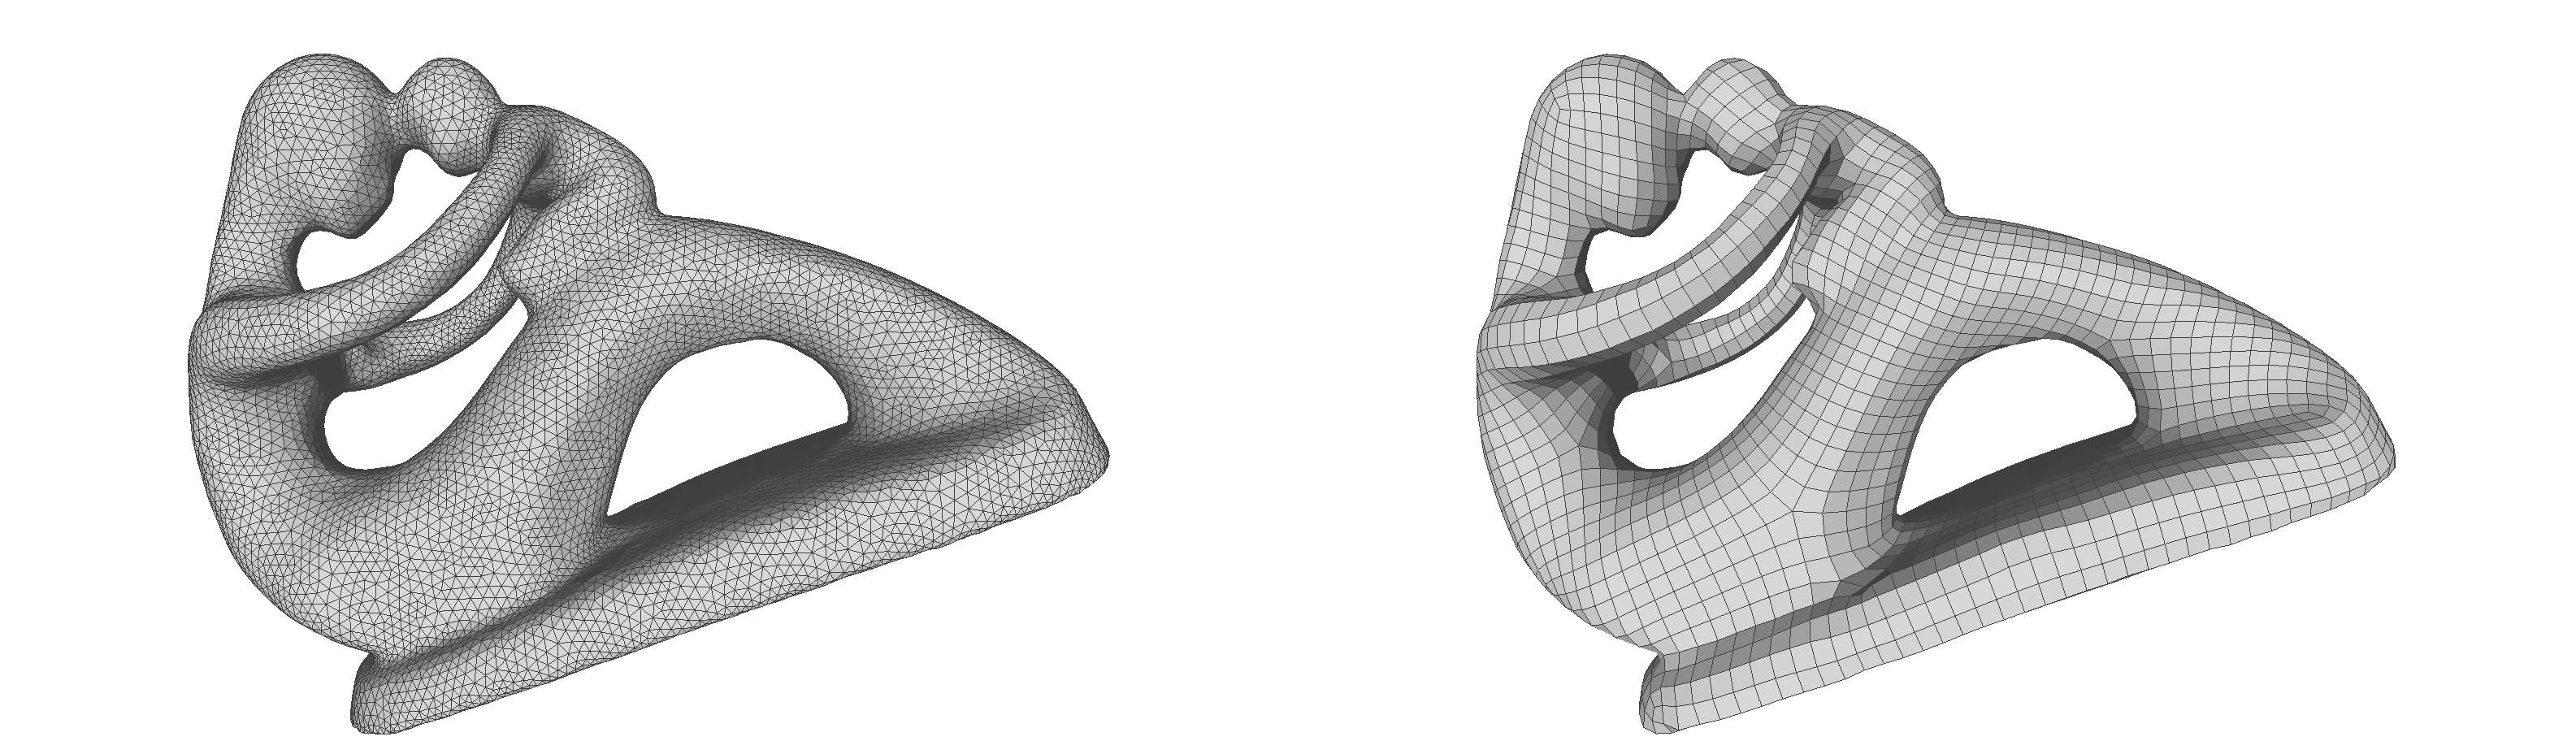
\includegraphics[width=15cm]{figures/tri_mesh_vs_quad_mesh.png}
\caption[Triangular mesh vs. Quad mesh]{A triangle-mesh (left) vs. a corresponding quad-mesh (right)}
\label{fig:tri_mesh_vs_quad_mesh}
\end{figure}
\subsection{Triangle Soup}
\label{sec:triangle_soup}
A \emph{triangle soup} is a formalization framework for describing a mapping of 2D manifold embedded in 3D onto the 2D Euclidean plane. In this formalization, every edge in the original mesh is treated as a cut seam, and therefore the input triangle-mesh is separated into individual triangles which are mapped onto the 2D domain.

\noindent Given that the input triangle-mesh is manifested as a tuple $M = (F,E,V)$, where $F$ is the set of facets, $E$ is the set of edges, and $V$ is the set of vertices, its triangle soup is given by $M_s = (F_s,E_s,V_s)$, where $\abs{F_s} = \abs{F}$, $\abs{E_s} = 2\abs{E} - \abs{E_{\partial M}}$, $\abs{V_s} = \sum_{v \in V} \mathrm{deg}(v) \cdot\abs{V}$, and $E_{\partial M}$ is the set of edges on the boundary of $M$ (if exists). Given a vertex $v_i$ of valence $k$ on $M$, and the triangle-fan adjacent to it (which constitutes a surface patch), we make the following notations:
\paragraph{Half-Edges} are two edges $e_i^k$ and $e_j^k$ on $M_s$ which corresponds to the same original edge $e_k$ on $M$.
\paragraph{Twin-Vertices} are any two vertices $v_i^k$ and $v_j^k$ on $M_s$ which corresponds to the same original vertex $v_k$ on $M$.
\noindent Figure \ref{fig:triangle_soup} illustrates a surface patch which is mapped into the 2D domain as a triangle soup.
\begin{figure}[ht]
\centering
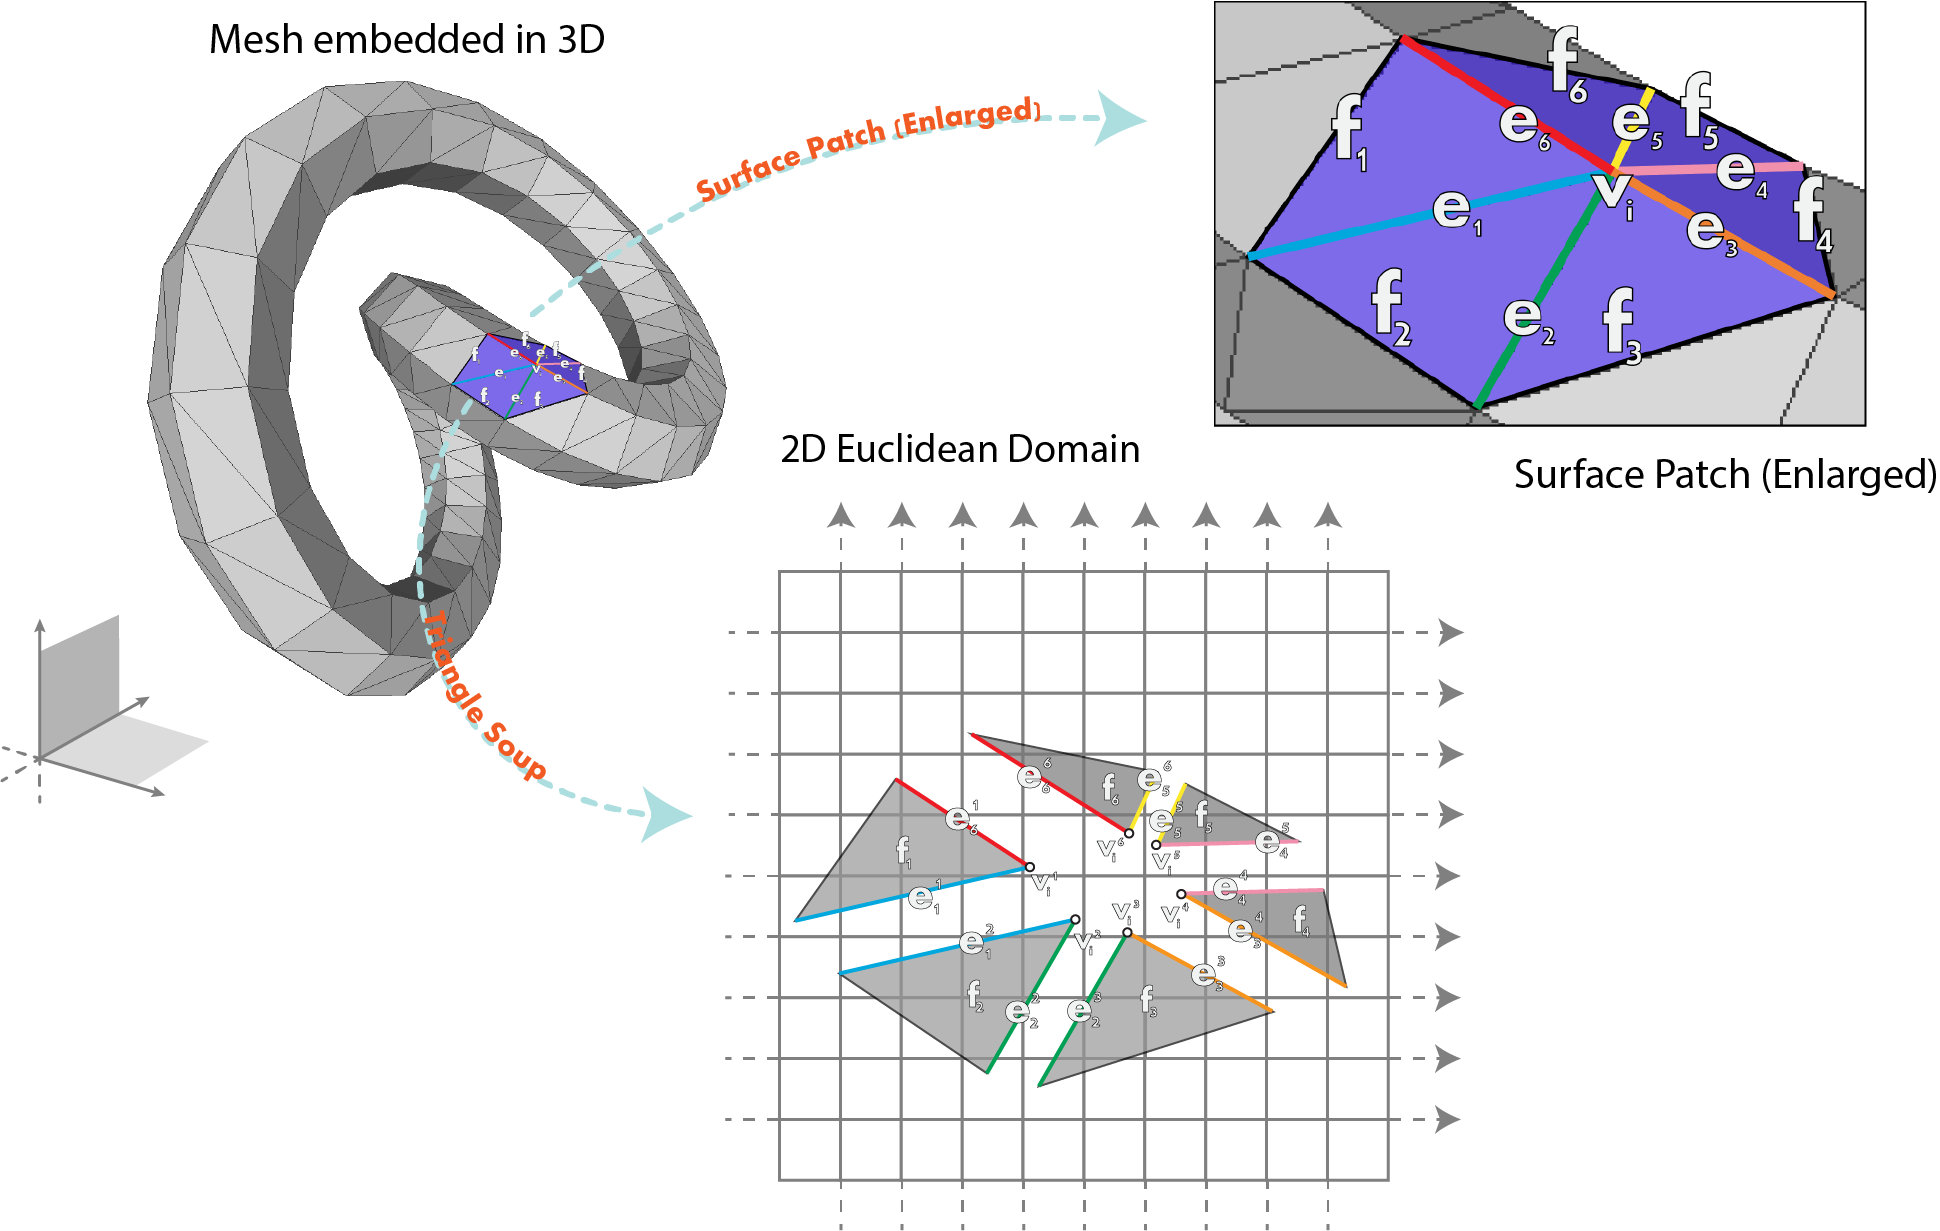
\includegraphics[width=16cm]{figures/triangle_soup.png}
\caption[Triangle Soup]{The purple surface patch, represented by the triangle-fan around the surface vertex $v_i$, is mapped onto the 2D Euclidean domain as a triangle soup. Half-edges are highlighted by the same color on the 2D domain, and twin-vertices are emphasized using a black stroked circle.}
\label{fig:triangle_soup}
\end{figure}
\subsection{Quad Meshes}
There are generally four types of quad meshes:
\begin{enumerate}
\item \textbf{Regular Quad Meshes} are quad meshes of which all their vertices are regular (valence 4). These type or meshes are relevant for disk or torodial (torus) topologies, and therefore, are limited in use.
\item \textbf{Semi-Regular Quad Meshes} are quad meshes which are made of 2D rectangular patches tessellated with quads, which are stitched together on the mesh's surface. This kind of meshes are highly useful due to their mostly regular nature (except for the possibly irregular vertices at the stitching points), but are also very hard to generate by remeshing methods.
\item \textbf{Valence Semi-Regular Quad Meshes} are quad meshes of which most of their vertices are of valence 4, but cannot be patched by stitching 2D patches. That is, a semi-regular quad mesh is also a valence semi-regular quad mesh, but not vice versa. These are the type of meshes which are usually produced by quad remeshing algorithms.
\item \textbf{Unstructured Quad Meshes} are quad meshes of which most of their vertices are irregular.
\end{enumerate}
\subsubsection{Irregular Vertices}
Irregular vertices are vertices of which their valence is different than 4. In other words, their immediate mesh neighbourhood do not resemble a 2D Cartesian grid. Quad remeshing techniques, on which we elaborate in the following chapters, produce valence semi-regular quad meshes which embed irregular vertices of valence 3 and 5 in order to compensate for Gaussian curvature. Figures \ref{fig:valence_3} and \ref{fig:valence_5} visualize the two types of irregular vertices.
\begin{figure}[ht]
\centering
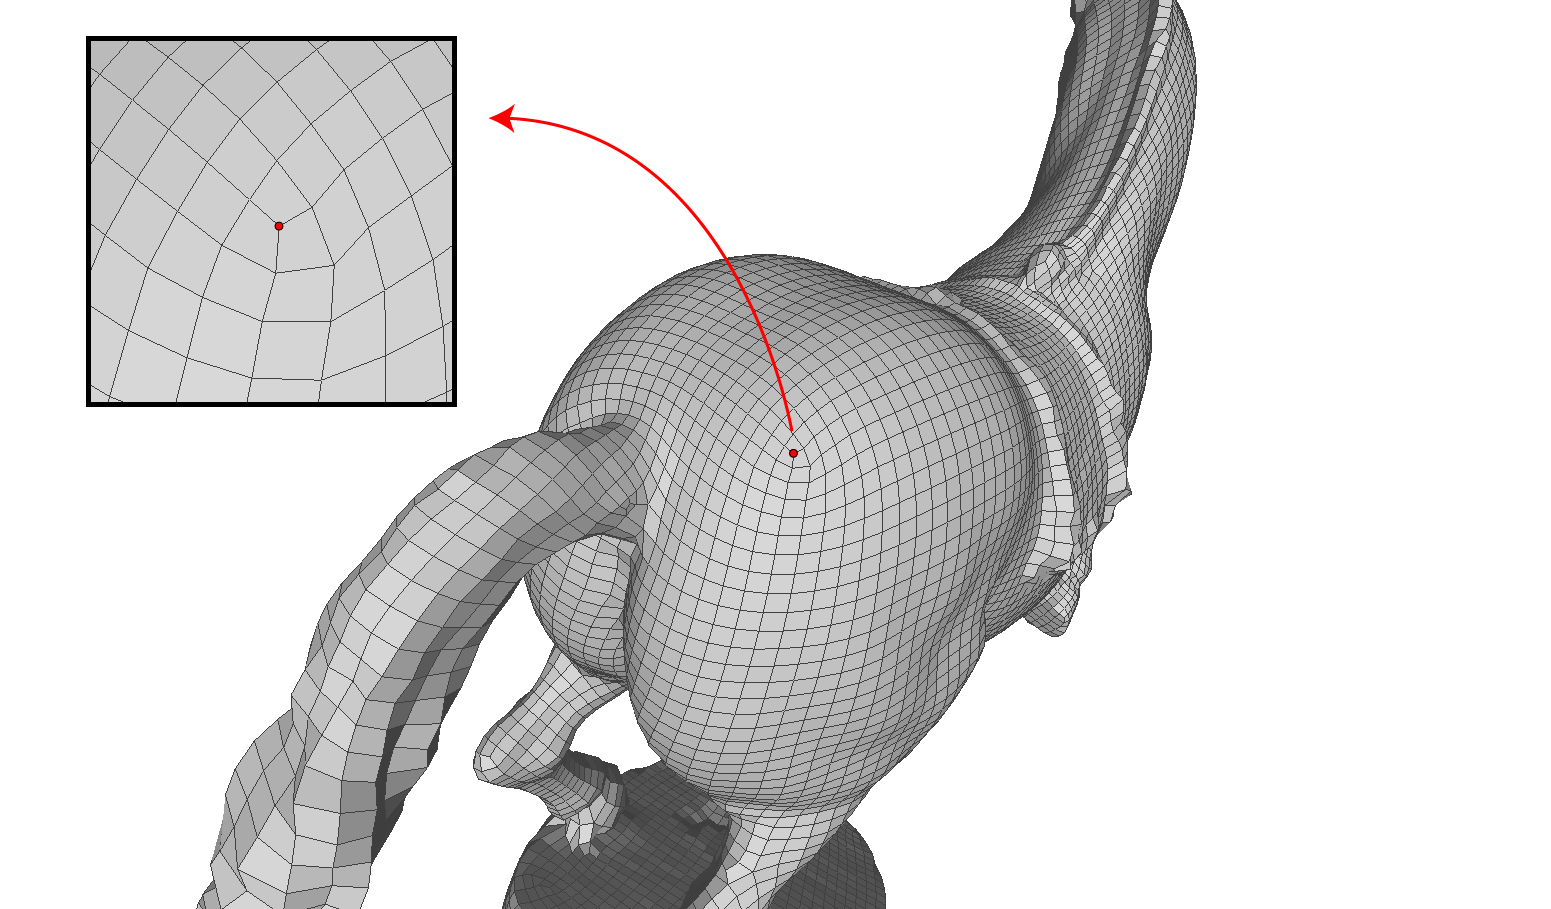
\includegraphics[width=13cm]{figures/valence_3.png}
\caption[Irregular vertex of valence 3]{The red dot indicates a vertex of valence 3 on the quadrangulated Rampant model}
\label{fig:valence_3}
\end{figure}
\begin{figure}[ht]
\centering
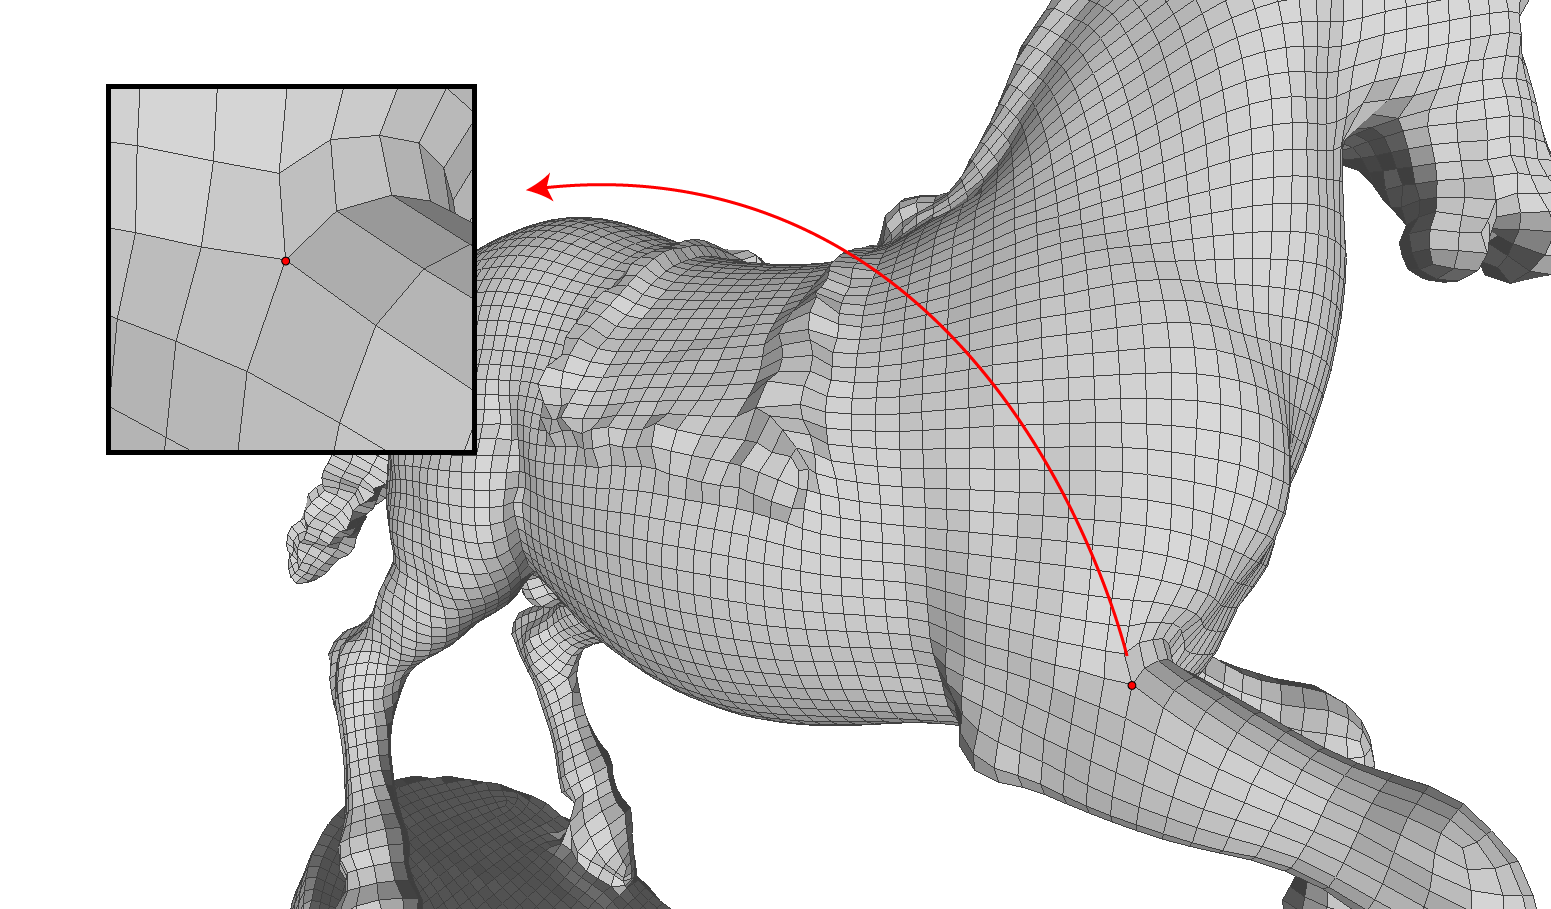
\includegraphics[width=13cm]{figures/valence_5.png}
\caption[Irregular vertex of valence 5]{The red dot indicates a vertex of valence 5 on the quadrangulated Rampant model}
\label{fig:valence_5}
\end{figure}
\subsubsection{Quad Mesh Quality}
Mesh models usually originates as unstructured triangle-meshes, and therefore, have to be converted into a semi-regular quad-meshes if the geometry-processing pipeline of a certain scenario requires it. In order to be able to compare between different conversion techniques, we have to define the quality measures, which are partially subjective, for a "good" quad-mesh.
\paragraph{Individual Quads Quality} If anisotropic quads are allowed or required, each quad should be close to
a 2D rectangle. Otherwise, it should be close to a 2D square. Specifically, it means that the the four vertices that make up the quads should be co-planar, opposite edges should have equal length and the four angles made up by consecutive edges should be close to $90^\circ$.
\paragraph{Curvature Alignment} Mesh edges should be oriented along curvature lines, except for points at flat areas where the curvature is zero.
\paragraph{Feature Alignment} Sharp geometric features of the mesh's surface should be traced by sequential mesh edges to get a quad mesh the approximates the original surface as good as possible.
\paragraph{Singular Points} The number of singular vertices, which are characterized by having valence an irregular valence (for example, 3 or 5), should be as small as possible, and their placement should be chosen or determined (automatically) such that the three former quality measures are maximized. Alternatively, their placement can be chosen to fit subjective artistic desires (for example, 3D character modeling).
\subsubsection{Applications}
Since points on smooth manifolds are characterized by two principal curvature directions (except for points on flat regions), quad-meshes are their natural approximators, since most vertices on a semi-regular quad-mesh are regular vertices of valence 4, of which their anti-symmetric edge pairs can be aligned with the principal curvature directions. This makes quad-meshes the desired approximations and representations of geometry in many types of applications.
\paragraph{3D Shape Modeling} In many cases, artists who design 3D models for entertainment and engineering purposes (video-games, animations, CAD, etc.) prefer to work in a quad-mesh settings, since their regular properties make it more intuitive to adapt their design to the geometric feature lines of their objects, which also provide better results under shape deformation.
\paragraph{Texturing} Since semi-regular quad-meshes are made of stitched together 2D rectangular quad grids, it is trivial to apply a set of textures and displacement-maps onto the 3D mesh.
\paragraph{Finite Element Simulations} Quad-meshes are preferred over triangle-meshes in finite-element simulation, since their regular nature reduce the approximation error and the number of mesh elements.
\paragraph{Shape Compression} The regular nature of quad-meshes, and especially of semi-regular quad-meshes, makes it possible to treat them as geometric images, due to their regularity, and apply on them image processing techniques such as image compression algorithms.
\section{Numerical Optimization}
Numerical optimization is a mathematical tool which grants its user the ability to minimize (or maximize) quantitative metric which usually measures the performance of the system under study. The metric to be optimized is expressed using a scalar objective which is a function of one or more system parameters. An \emph{optimization problem} is a problem which is satisfied by finding a point in the problem's domain where the objective metric is minimized (or maximized) locally or globally. Since we usually cannot find an analytic expression for the solution of an optimization problem, we have to solve it by iterative progression towards the solution using local approximations of the objective function in hand. An algorithm which iteratively converges to the solution is called an \emph{optimization method}. Numerical optimization methods are fundamental tools in all fields of engineering and science.

\noindent An optimization problem which has no restrictions on its domain is called an \emph{unconstrained optimization problem}. If we require that the solution will be restricted to a certain region of the domain, the problem is then called a \emph{constrained optimization problem}. Methods for solving unconstrained optimization problems are divided into two main types:
\begin{itemize}
    \item Trust Region Methods
    \item Line Search Methods
\end{itemize}
The following subsection contains a quick review for the two most common line-search unconstrained optimization methods: \emph{Gradient Descent} and \emph{Newton's Method}, of which we specifically use in the context of this work. For more information about Numerical Optimization, please refer to \cite{Nocedal2006Numerical}.
\paragraph{Important Remark} Every optimization problem can be formulated both as a minimization problem (by minimizing the objective function) or as a maximization problem (by maximizing the negative objective function). In this text, we assume that all optimization problems are formulated as minimization problems.
\subsection{Quadratic Approximation}
Given a scalar function:
$$f:\mathbb{R}^2\rightarrow\mathbb{R}$$
We know by the multivariate Taylor's theorem that its quadratic approximation $q\left(x,y\right)$ at the point $\left(x_0,y_0\right)$ is given by:
\begin{equation}\label{quadratic_approx}
\begin{split}
f\left(x,y\right) \approx f\left(x_0,y_0\right) + f_x\left(x_0,y_0\right)\left(x - x_0\right) + f_y\left(x_0,y_0\right)\left(y - y_0\right) \\ + \frac{1}{2}f_{xx}\left(x_0,y_0\right)\left(x - x_0\right)^2 + \frac{1}{2}f_{xy}\left(x_0,y_0\right)\left(x - x_0\right)\left(y - y_0\right) \\ +  \frac{1}{2}f_{yx}\left(x_0,y_0\right)\left(x - x_0\right)\left(y - y_0\right) + \frac{1}{2}f_{yy}\left(x_0,y_0\right)\left(y - y_0\right)^2
\end{split}
\end{equation}
By factorizing (\ref{quadratic_approx}) we get the following:
\begin{equation}\label{factorized_quadratic_approx}
\begin{split}
f\left(x,y\right) \approx f\left(x_0,y_0\right) + f_x\left(x_0,y_0\right)\left(x - x_0\right) + f_y\left(x_0,y_0\right)\left(y - y_0\right) \\ + \frac{1}{2}\Big(\left(x - x_0\right)\big( f_{xx}\left(x_0,y_0\right) \left(x - x_0\right) + f_{xy}\left(x_0,y_0\right) \left(y - y_0\right) \big) \\ + \big( f_{yx}\left(x_0,y_0\right) \left(x - x_0\right) + f_{yy}\left(x_0,y_0\right) \left(y - y_0\right) \big)\left(y - y_0\right)\Big)
\end{split}
\end{equation}
By denoting:
$$
p = 
\begin{pmatrix}
x\\
y\\
\end{pmatrix},
p_0 = 
\begin{pmatrix}
x_0\\
y_0\\
\end{pmatrix},
\nabla f\left(x_0,y_0\right) = 
\begin{pmatrix}
f_x\left(x_0,y_0\right)\\
f_y\left(x_0,y_0\right)\\
\end{pmatrix},
\nabla^2 f\left(x_0,y_0\right) = 
\begin{pmatrix}
f_{xx}\left(x_0,y_0\right) & f_{xy}\left(x_0,y_0\right)\\
f_{yx}\left(x_0,y_0\right) & f_{yy}\left(x_0,y_0\right)
\end{pmatrix}
$$
We can rewrite (\ref{vectorized_quadratic_approx}) in a vectorized form by:
\begin{equation}\label{vectorized_quadratic_approx}
\begin{split}
f\left(p\right) \approx f\left(p_0\right) + \nabla f\left(p_0\right)^T\left(p-p_0\right) + \frac{1}{2}\left(p-p_0\right)^T\nabla^2 f\left(p_0\right)\left(p-p_0\right)
\end{split}
\end{equation}
\noindent The right side of (\ref{vectorized_quadratic_approx}) is called the \emph{quadratic approximation} of $f(p)$ at the point $p=(x_0, y_0)$, and is denoted by $Q(p)$.

\noindent The derivation above was done for the two-dimensional case, however, it is possible to generalize the derivation and show that the vectorized end result is the same for $f:\mathbb{R}^n\rightarrow\mathbb{R}$ with an arbitrary $n$.

\noindent The geometric interpretation of the quadratic approximation of a function at a point $p_0$ is a hyper-paraboloid that passes through $p_0$ which best approximates the function $f(p)$ around any small neighbourhood of $p_0$.
\begin{figure}[ht]
\centering
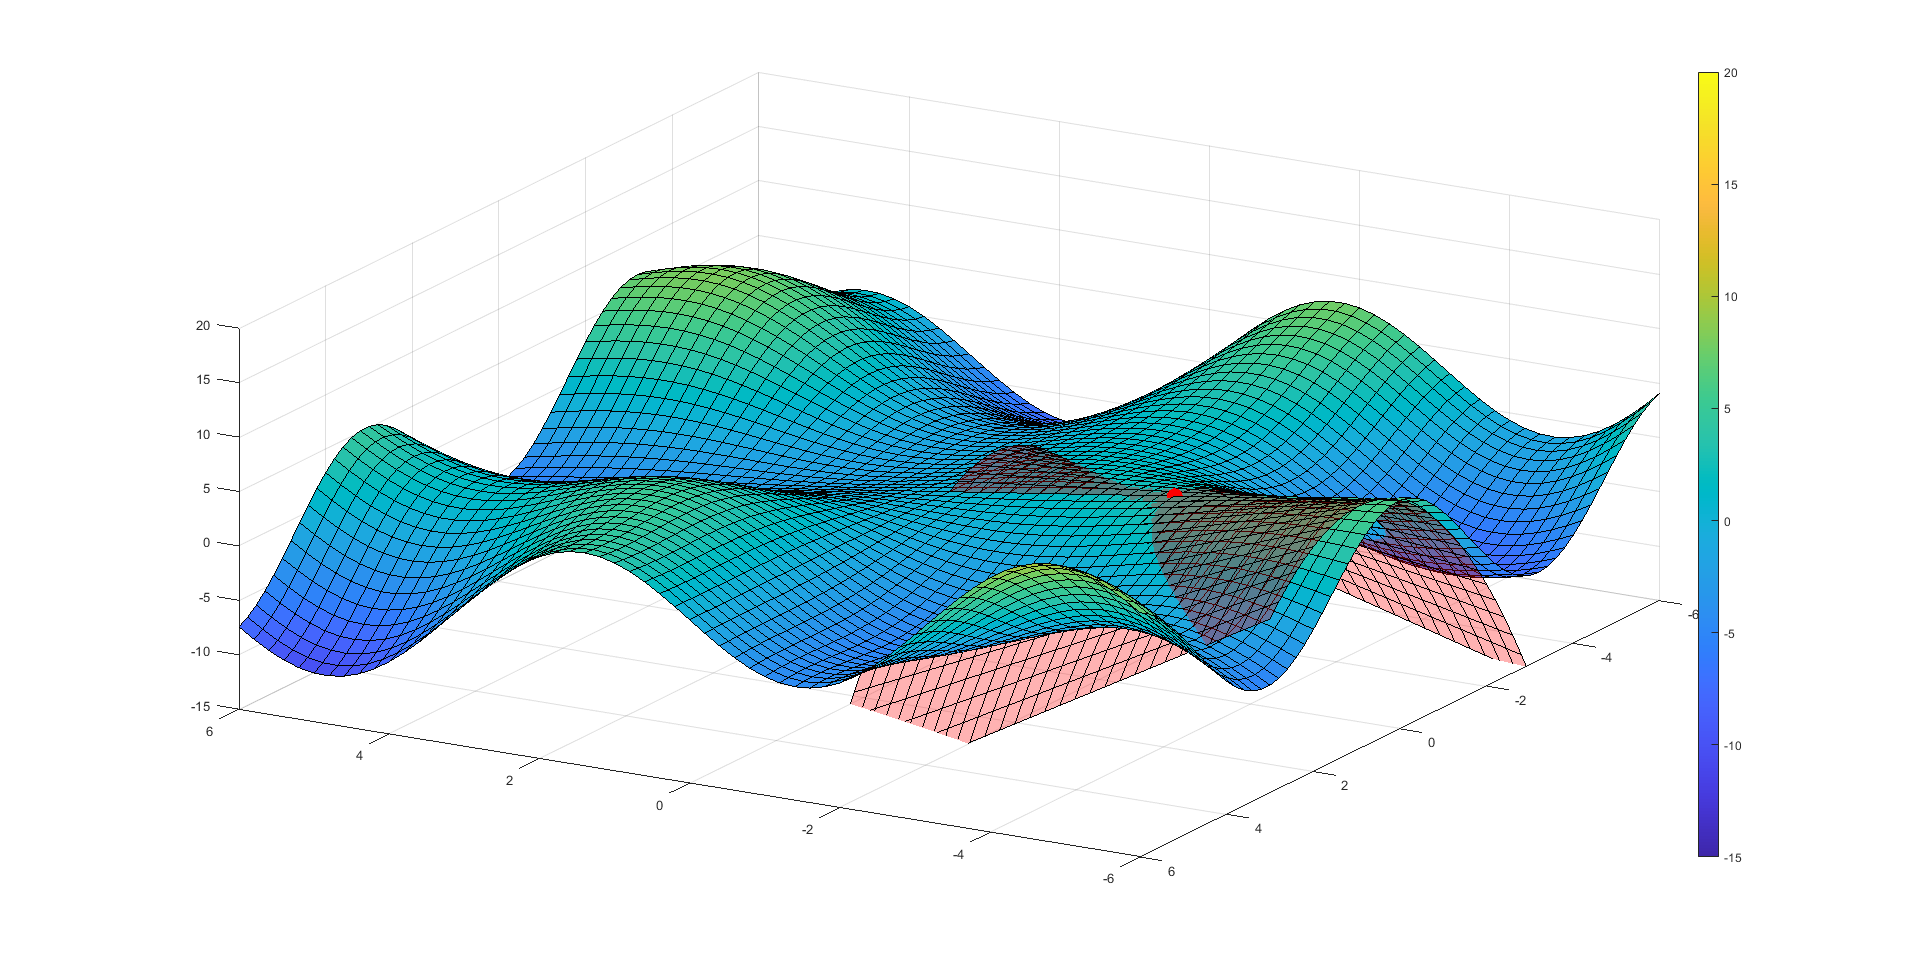
\includegraphics[width=13cm]{figures/quad_approx1}
\caption[Quadratic approximation example 1]{Example plot of the quadratic approximation (the red paraboloid) of the function $f\left(x_0, x_1\right) = x_2sin\left(x_1\right) - x_1cos\left(x_2\right)$ at the point $p_0 = \left(4.4, 0.4\right)$ (the red dot)}
\label{fig:quad_approx1}
\end{figure}
\begin{figure}[ht]
\centering
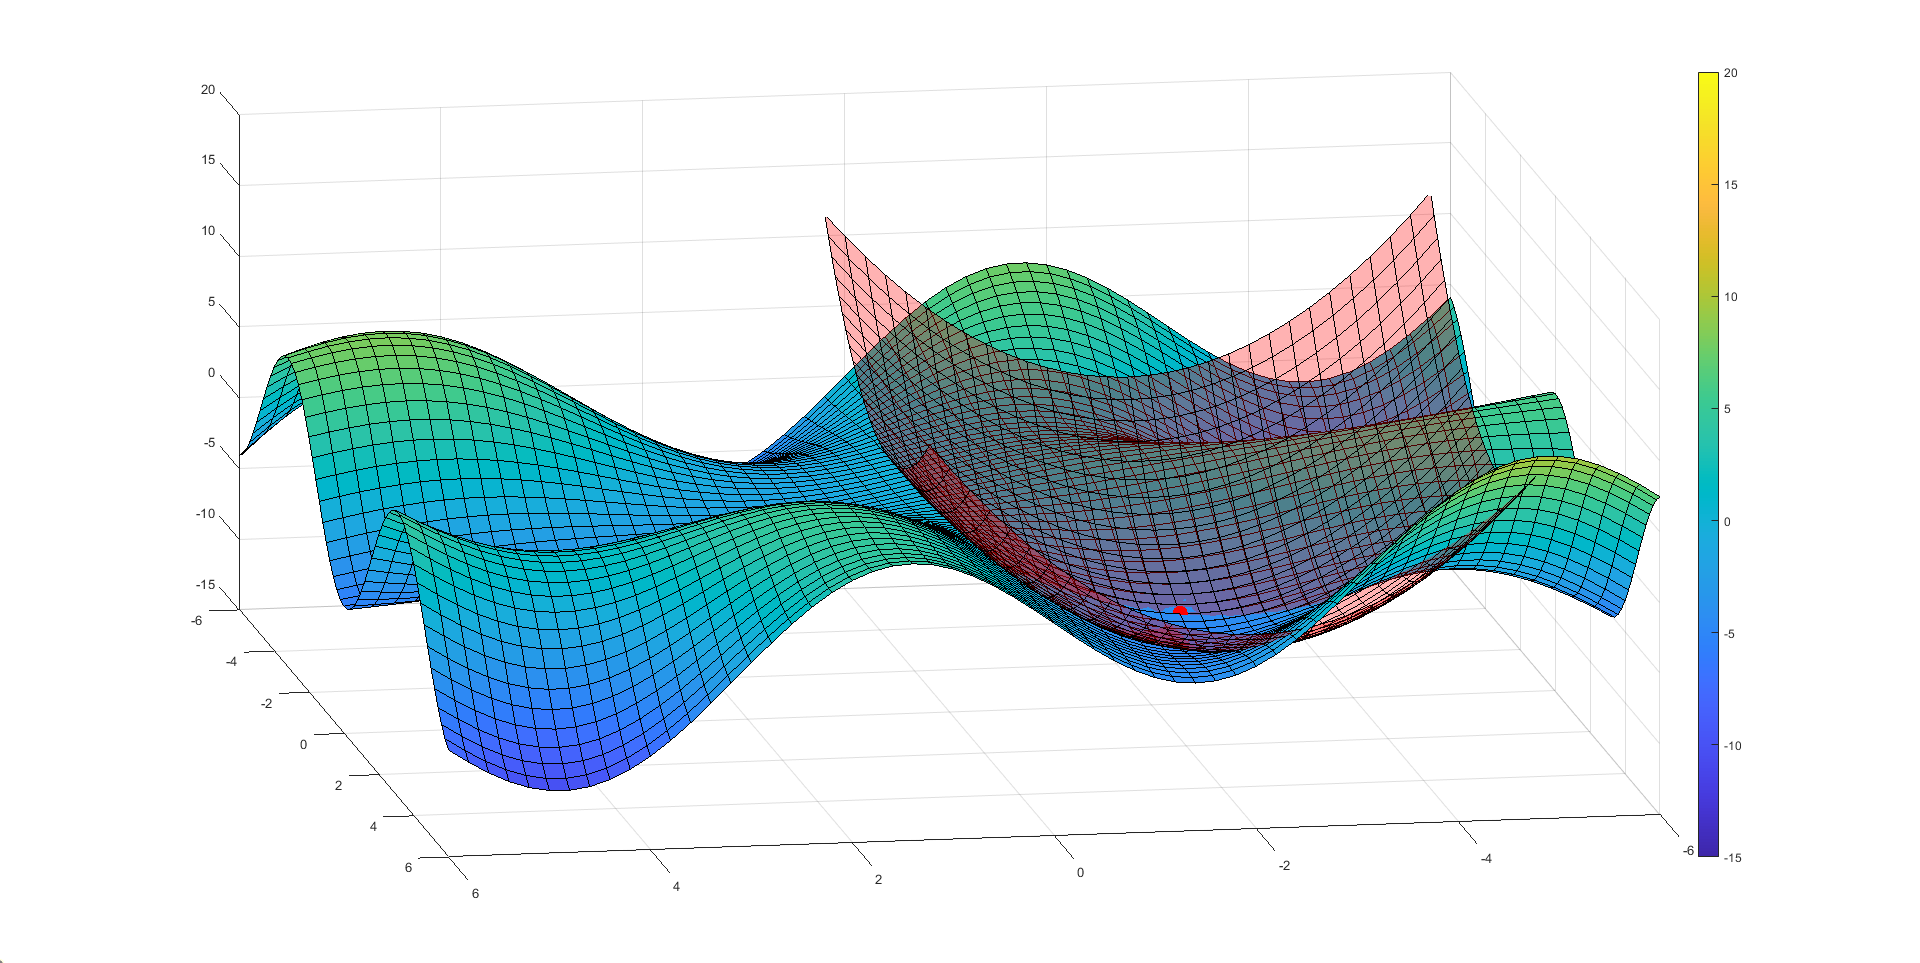
\includegraphics[width=13cm]{figures/quad_approx2}
\caption[Quadratic approximation example 2]{Another example plot of the quadratic approximation (the red paraboloid) of the function $f\left(x_0, x_1\right) = x_2sin\left(x_1\right) - x_1cos\left(x_2\right)$ at the point $p_0 = \left(-1.8, 2.8\right)$ (the red dot)}
\label{fig:quad_approx2}
\end{figure}
\subsection{Linear Approximation}
By omitting the quadratic form from equation (\ref{vectorized_quadratic_approx}) to we get:
\begin{equation}\label{vectorized_linear_approx}
\begin{split}
f\left(p\right) \approx f\left(p_0\right) + \nabla f\left(p_0\right)^T\left(p-p_0\right)
\end{split}
\end{equation}
\noindent The right side of (\ref{vectorized_linear_approx}) is called the \emph{linear approximation} of $f(p)$ at the point $p=(x_0, y_0)$, and is denoted by $L(p)$.

\noindent The geometric interpretation the linear approximation of a function at a point $p_0$ is a hyperplane that passes through $p_0$ which best approximates the function $f(p)$ around any small neighbourhood of $p_0$.
\begin{figure}[ht]
\centering
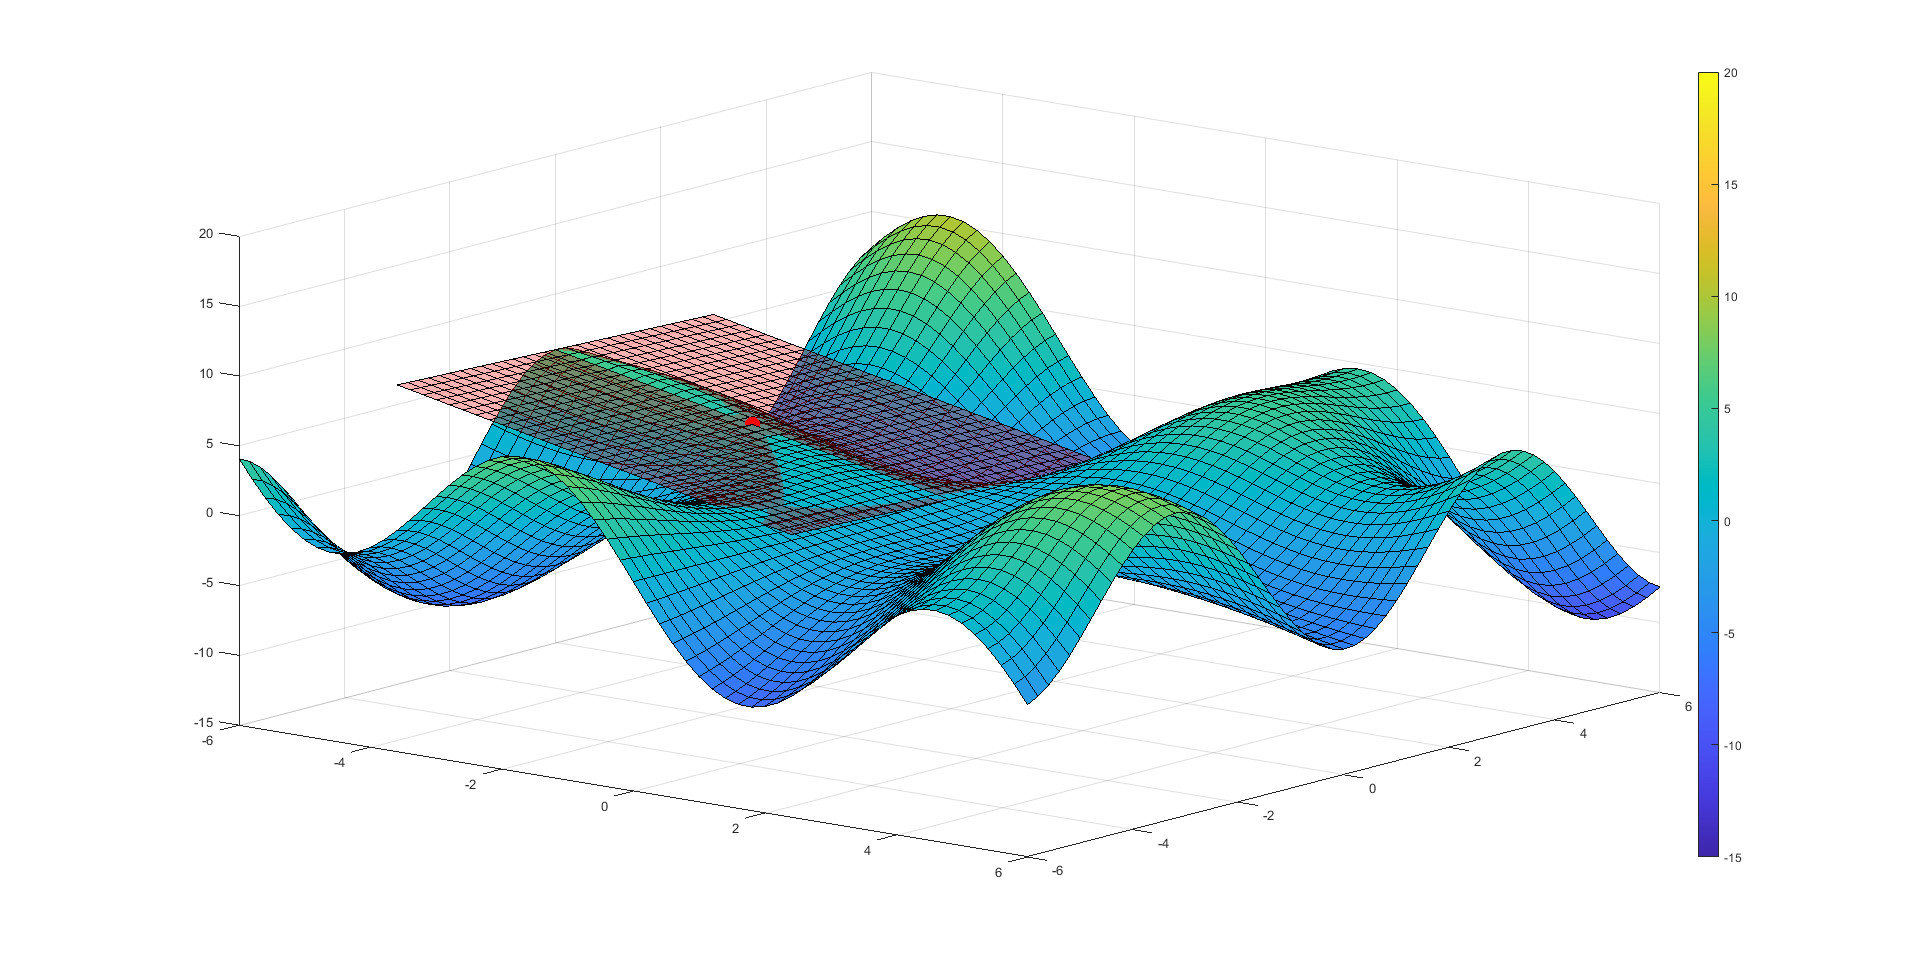
\includegraphics[width=13cm]{figures/linear_approx1}
\caption[Linear approximation example 1]{Example plot of the linear approximation (the red plane) of the function $f\left(x_0, x_1\right) = x_2sin\left(x_1\right) - x_1cos\left(x_2\right)$ at the point $p_0 = \left(0, -3\right)$ (the red dot)}
\label{fig:linear_approx1}
\end{figure}
\begin{figure}[ht]
\centering
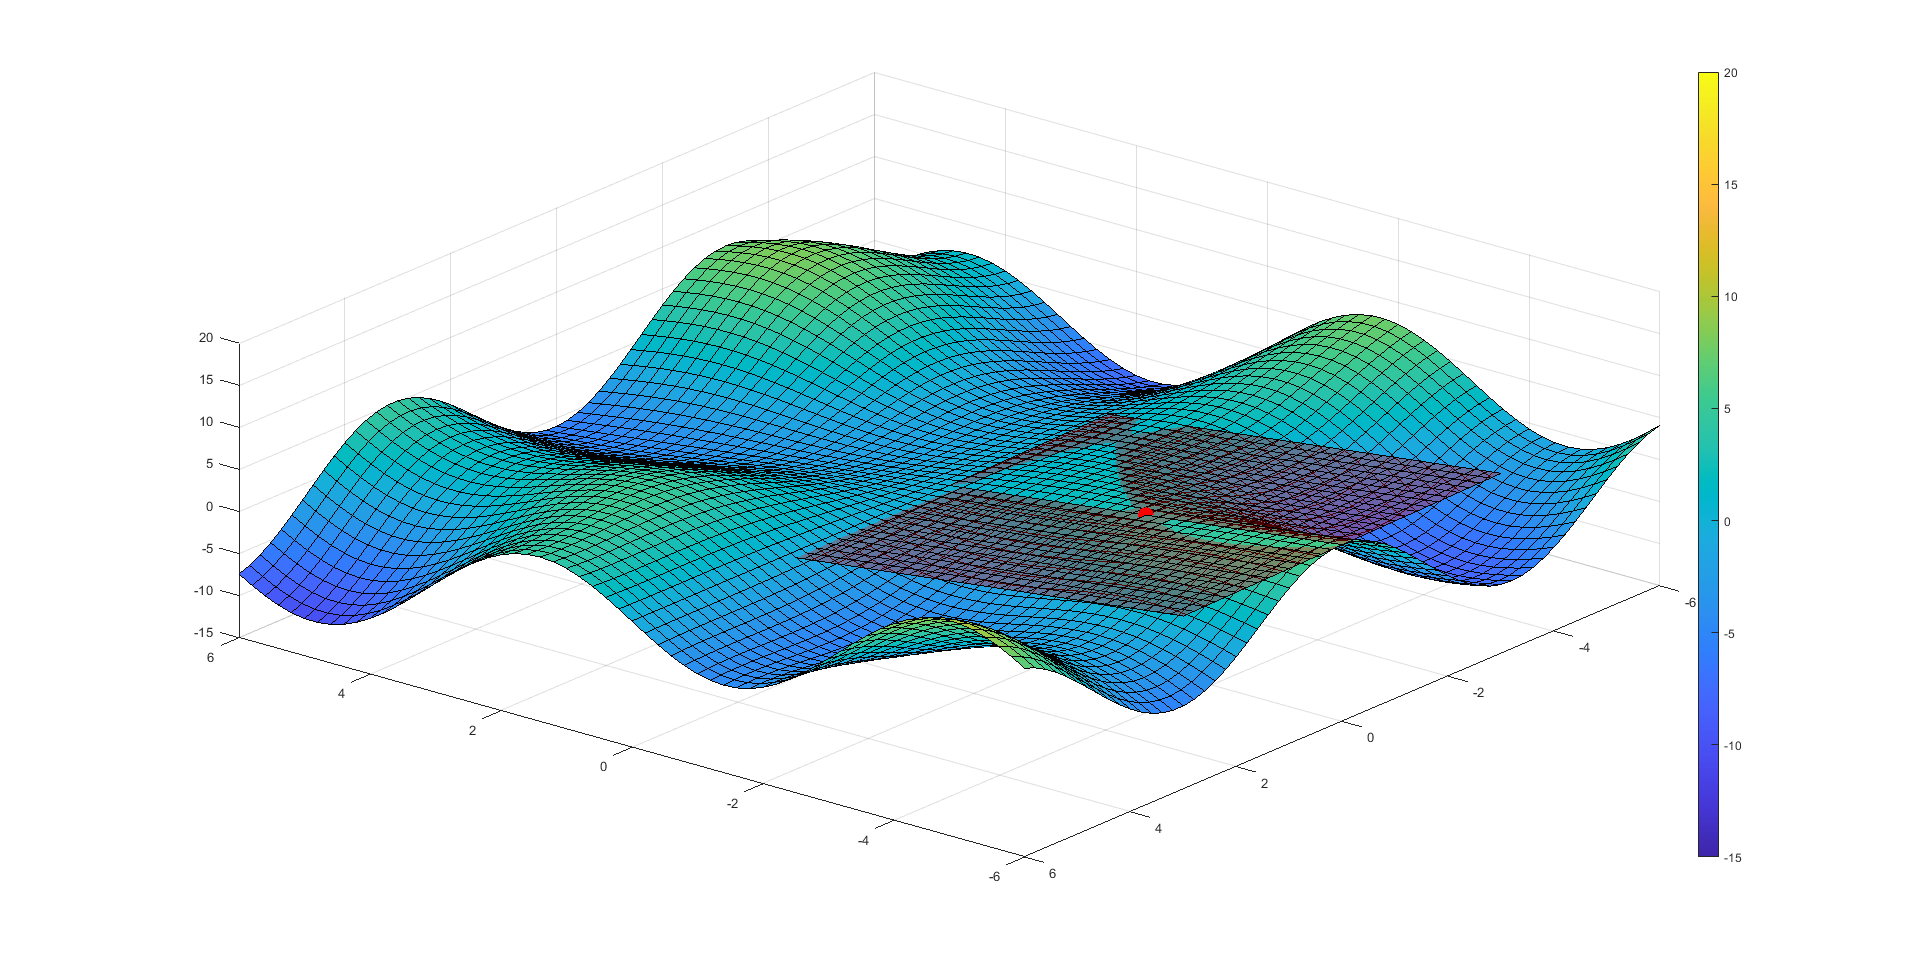
\includegraphics[width=13cm]{figures/linear_approx2}
\caption[Linear approximation example 2]{Plot from a different angle of the same linear approximation from figure \ref{fig:linear_approx1}}
\label{fig:linear_approx2}
\end{figure}
\subsection{Gradient Descent}
Gradient Descent is a first-order iterative line-search algorithm, of which at its $i$th iteration takes a single step in the direction of $-\nabla f\left(p_i\right)$ (the negative gradient direction, calculated at the point $p_i$). To see why, assume that we're given a function $f:\mathbb{R}^n\rightarrow\mathbb{R}$ and a point $p_i$ in its domain. We would like to find a new point $p_{i+1}$, which together with $p_i$, will provide the direction of steepest descent on the linear approximation of $f(p)$ at the point $p_i$. The linear approximation of $f$ at $p_i$ is given by:
\begin{equation}
\label{vectorized_quadratic_approx_p}
\begin{split}
L\left(p\right) = f\left(p_i\right) + \nabla f\left(p_i\right)^T\left(p-p_i\right)
\end{split}
\end{equation}
Let's denote $d_i = p-p_i$. By the definition of the inner-product, if we take $d_i = -\widehat{\nabla f}\left(p_i\right)$ as unit-vector that represent the direction of progression, we will achieve maximal decrease in $L\left(p\right)$ out of all possible unit-vector directions. This mean that we would like to choose $p_{i+1}$ somewhere along the ray emitted from $p_i$ in direction $-\widehat{\nabla f}\left(p_i\right)$. That is, we're looking for a step-size $\alpha_i>0$ such that by  taking $p_{i+1}=p_i - \alpha \widehat{\nabla f}\left(p_i\right)$ we will achieve a sufficient decrease in $f\left(p_{i+1}\right)$. That quest for finding the correct step-size along a ray is called \emph{Line Search}.
Pseudo-code for the vanilla versions of the Line-Search and Gradient Descent algorithms are given in Algorithms \ref{alg:line_search_algorithm} and \ref{alg:gradient_descent_algorithm}, respectively. The Gradient Descent algorithm converges linearly to a local minimum point of $f$. However, there is always a risk that the process get to a sudden halt at a saddle point, where the gradient is zero. For further reading, please refer to \cite{Nocedal2006Numerical}.
\begin{algorithm}[ht]
  \caption{Line Search Algorithm}
  \label{alg:line_search_algorithm}
  \begin{algorithmic}[1]
    \Function {LineSearch}{$f$, $p$, $d$, $\alpha_0$}
    \State $\emph{sufficient} \leftarrow false$
    \State $\alpha \leftarrow \alpha_0$
    \State $v \leftarrow f\left(p\right)$
    \Repeat
        \State $p_{next} \leftarrow p + \alpha d$
        \State $v_{next} \leftarrow f\left(p_{next}\right)$
        \State $\alpha \leftarrow \frac{\alpha}{2}$
        \If {$v_{next} < v$}
            \State $\emph{sufficient} \leftarrow true$
        \EndIf
    \Until{$\emph{sufficient}$}
    \State \Return $p_{next}$
    \EndFunction
  \end{algorithmic}
\end{algorithm}
\begin{algorithm}[ht]
  \caption{Gradient Descent Algorithm}
  \label{alg:gradient_descent_algorithm}
  \begin{algorithmic}[1]
    \Function {GradientDescent}{$f$, $\nabla f$, $p_0$, $\alpha$, $\epsilon$}
      \State $i \leftarrow 0$
      \While{$ \norm{ \nable f \left( p_i \right) }_2 > \epsilon$}
        \State $d_i \leftarrow -\nabla f \left(p_i\right)$
        \State $p_{i+1} \leftarrow \Call{LineSearch}{f, p_i, d_i, \alpha}$
        \State $i \leftarrow i + 1$
      \EndWhile
      \State \Return $p_i$
    \EndFunction
  \end{algorithmic}
\end{algorithm}
\subsection{Newton's Method}
Newton's Method is a second-order iterative line-search algorithm. In contrast to the Gradient Descent algorithm, which is based on the linear (first order) approximation of $f$ at point $p_i$, Newton's Method is based on the quadratic (second order) approximation of $f$ at point $p_i$. If the quadratic approximation of $f$ at a given point is a convex hyper-paraboloid, it has a minimum point $q_{min}$. Since a quadratic approximation of a function $f$, at point $p_i$, gives a good approximation of $f$ at a small neighbourhood of $p_i$, it make sense that by stepping along the ray (in $f$'s domain space) emitted from $p_i$ in direction $d_i = q_{min} - p_i$ will yield a new point $p_{i+1}$ which provide sufficient decrease in $f$.
In order to determine $d_i$, we first have to find the minimum point of the quadratic approximation of $f$ at point $p_i$. By equation (\ref{vectorized_quadratic_approx}), we know that the quadratic approximation of $f\left(p_i\right)$ is given by:
\begin{equation}\label{vectorized_quadratic_approx_p}
\begin{split}
Q\left(p\right) = f\left(p_i\right) + \nabla f\left(p_i\right)^T\left(p-p_i\right) + \frac{1}{2}\left(p-p_i\right)^T\nabla^2 f\left(p_i\right)\left(p-p_i\right)
\end{split}
\end{equation}
We first note that:
\begin{equation}\label{d_i_p_i_p}
\begin{split}
d_i = p - p_i \implies p = p_i + d_i
\end{split}
\end{equation}
Plugging \ref{d_i_p_i_p} into equation \ref{vectorized_quadratic_approx_p}, we get:
\begin{equation}\label{vectorized_quadratic_approx_p_i_d_i}
\begin{split}
Q\left(p_i + d_i\right) = f\left(p_i\right) + \nabla f\left(p_i\right)^Td_i + \frac{1}{2}d_i^T\nabla^2 f\left(p_i\right)d_i
\end{split}
\end{equation}
By differentiating equation \ref{vectorized_quadratic_approx_p_i_d_i} by $d_i$, we get that:
\begin{equation}\label{newton_equation}
\begin{split}
\nabla Q\left(p_i + d_i\right) = \nabla f\left(p_i\right) + \nabla^2 f\left(p_i\right)d_i
\end{split}
\end{equation}
By setting $\nabla Q\left(p_i + d_i\right) = 0$ (in order to find the minimum point) and plugging back into equation \ref{newton_equation}, we get that:
\begin{equation}\label{newton_equation}
\begin{split}
d_i = -\nabla^2 f\left(p_i\right)^{-1} \nabla f\left(p_i\right)
\end{split}
\end{equation}
Equation \ref{newton_equation} gives us an explicit expression for the vector $d_i$, which takes us from the point $p_i$, to the minimum point of the paraboloid which forms the quadratic approximation of $f$ at point $p_i$. By expanding this idea further, we can normalize $d_i$ to be a unit vector, and use it as a direction of search for a line-search method.
\paragraph{Important Remark} In order for the quadratic approximation of $f$ in point $p_i$ to have minimum point, its Hessian $\nabla^2 f\left(p_i\right)$ has to be positive semi-definite matrix, which means that it has to have non-zero singular values. The geometric meaning of that, is that the hyper-paraboloid represented by the quadratic approximation of $f$ in $p_i$ should be convex. In case it doesn't, we can use the \emph{singular-value decomposition} to reassemble $\nabla^2 f\left(p_i\right)$ into its closest approximation which doesn't have any non-zero singular value, and use that approximation to solve the sparse linear system of equations, and extract the current direction of descent $d_i$. For more information about the singular-value decomposition, please see \cite{strang2006linear}.

\noindent Pseudo-code for a vanilla version of the Newton's Method algorithm is given in Algorithm \ref{alg:newton_method_algorithm}. The Newton's Method algorithm converges quadratically to a local minimum point of $f$, given certain conditions are met. For further reading, please refer to \cite{Nocedal2006Numerical}.
\begin{algorithm}[ht]
  \caption{Newton's Method Algorithm}
  \label{alg:newton_method_algorithm}
  \begin{algorithmic}[1]
    \Function {NewtonMethod}{$f$, $\nabla f$, $p_0$, $\alpha$, $\epsilon$}
      \State $i \leftarrow 0$
      \While{$\norm{\nable f\left(p_i\right)}_2 > \epsilon$}
        \State $d_i \leftarrow -\nabla^2 f\left(p_i\right)^{-1} \nabla f\left(p_i\right)$
        \State $p_{i+1} \leftarrow \Call{LineSearch}{f, p_i, d_i, \alpha}$
        \State $i \leftarrow i + 1$
      \EndWhile
      \State \Return $p_i$
    \EndFunction
  \end{algorithmic}
\end{algorithm}
\chapter{Research Motivation}

\section{Research Motivation}
Geometry processing is the hidden engine that propels many design tools used by the graphics-related industry. Shape deformation, remeshing, surface parameterization, texture synthesis and so forth \cite{PMP:2010} are some of the standard tasks within the geometry processing field. Geometry processing algorithms play key roles in the process of content creation, from the initial shaping of an object, through texturing and animation, to final analysis and further enhancements. Their purpose is to assist the artist in realizing a design that fits their vision, with the least effort possible. Yet, even with the most advanced algorithms, the design process is often long and tedious. It requires many trial-and-error iterations, tweaking and experimenting with parameters, improving and optimizing, until a desired result is achieved. Researchers are constantly attempting to improve the automation of the design process, to whatever extent possible, in order to ameliorate the burden of realizing a design. To do so, they attempt to deduce and predict potential objectives a designer might have, formulate optimization problems that represent those objectives, and compute optimal solutions for these representative problems. This approach is very appealing from a development perspective: the algorithm does not have to be efficient or have a user interface, since it is automatic. However, while automatic solutions may work in certain cases, in many other cases this approach is unhelpful, or even misguided. Designers often begin without a clearly defined objective and  decide, while exploring and experimenting with designs, when the result is satisfactory -- an ``\emph{I know it when I see it}" type of process. This phrase also serves to underline the difficulty inherent in the fact that some objectives are, in fact, \emph{subjective}.  Conversely, in some cases the designers \emph{do know} what they want, but the algorithm will continue suggesting a different design, because it better fits a set of preconceived objectives. This, obviously, leads to frustration and contradicts the very purpose that the tool was developed to accomplish: to aid the designer.

\noindent An alternative approach would be to develop systems for \emph{Guided Optimization}, where the user and the computer work together towards achieving the goal.

\noindent Guided optimization, also known as human-in-the-loop optimization, is possible when the algorithm manifests the three following properties:
\begin{enumerate}
\item It is responsive
\item It is predictable
\item It has an intuitive user interface
\end{enumerate}

\section{Guided Optimization}
\paragraph*{Responsiveness}
Responsiveness is the ability of an algorithm to react to input from the user in an interactive system. Normally, when developing a new optimization method, the aim is to converge to a minimum as quickly as possible. Iterative optimization processes require a certain number of iterations to converge, where each iteration requires a certain amount of time, thus reduction of the total time is the main goal. An important fact to consider is that optimizers cannot typically react to new input mid-step, so the duration of an iteration in a responsive algorithm should not be too long, i.e., the iterations should be \emph{efficient}. A rule of thumb is that 5-10 iterations per second is the minimal number that is still considered interactive. On the other hand, the optimizer should also be \emph{effective}, that is, each step should make sufficient, ideally clearly visible, progress. These two properties, efficiency and effectiveness, usually come at the expense of one another. The challenge in developing a guided optimization is to find or construct an algorithm that balances the two well. 

For example, two well-known methods for surface parameterization are the quasi-Newton method from \cite{Smith:2015}, and the second-order cone programming (SOCP) method from \cite{Lipman:2012}. A quasi-Newton step takes a fraction of the time that an SOCP step takes, but the quasi-Newton method usually requires thousands of iterations to converge, while the SOCP approach usually requires less than ten. Nevertheless, even though the total time the SOCP approach requires is generally shorter, it can not be used for guided optimization, since the duration of each individual iteration is too long. The quasi-Newton method cannot be used either, simply because it is not effective enough. In \cite{Poranne:Autocuts:2017}, we found that the composite majorization approach strikes the right balance for small sized meshes. Handling of large sized meshes is discussed in this proposal later.

\paragraph*{Predictability}
During the interaction with a guided-optimization system, it is very important that the effects of a certain action are predictable. The problems we solve are normally formulated with many constraints and have many local minima. A small variation in the input can easily cause the optimizer to fall unexpectedly into a local minimum, produce dramatic changes in the result, and ruin the design-in-progress. The problem is further exacerbated in the presence of discrete variables or objectives. These occurrences are extremely frustrating to a designer and can easily cause a simple project to become painstaking and time-consuming. My approach to avoiding this problem is to allow the constraints to be violated in a controllable manner. One way to do so is by utilizing the continuation method, as explained below.

\paragraph*{User interface}
A guided optimization system requires a user-friendly interface. A user interface in this context is more than just a graphics display with text boxes for parameters, but rather a mechanism that allows a user to trace curves, make gestures with the mouse, and express their wishes in a much more refined and subtle manner. The design of such interfaces is an arduous task, and unfortunately one that is not often discussed in scientific papers. A well-designed user interface has the potential to render a problem much more manageable, even without the use of powerful optimization, while a poorly-designed one can leave the user feeling frustrated and unsatisfied with the results, even though it may be running a powerful algorithm behind the scenes. The investigation and optimization of user interfaces is much less structured than other computational problems. In the following section, I will present a few relevant examples.

\section{Guided Optimization for Quad Remeshing}
Inspired by \cite{Poranne:Autocuts:2017}, which formulated the problem of UV mappings as a guided optimization problem, we make an attempt, in this work, to formulate the problem of \emph{Quad Remeshing} as a guided optimization problem.
Many applications in computer graphics, such as character modeling and animation, architectural geometry, and physical simulation to some extent, call for quad meshes as a representation of the geometry. However, since triangle meshes are generally more prevalent and are naturally the type of mesh generated by object acquisition and surface reconstruction methods, they need to be converted to a quad mesh via the process known as quad remeshing. In the following chapters, we give a brief overview of related works in the field of quad remeshing, and describe in detail our own approach and contribution for the solution of this problem.

\chapter{Related Work}

A lot of effort has been put in the last decades to develop efficient algorithms and tools for converting a triangle-mesh into a quad-mesh (also known as \emph{mesh quadrangulation}). Since there is a detailed and nice survey on quad-mesh generation and processing \cite{10.1111/cgf.12014}, we will give a very brief review of the two main families of quadrangulation techniques.

\section{Quad Conversion}
\emph{Quad Conversion} is a type of method which directly converts a triangle-mesh into a quad-mesh by explicitly manipulating the mesh's elements connectivity. A naive method to convert any polygonal mesh into a quad-mesh is to perform a single iteration of Catmull-Clark subdivision \cite{Catmull1978RecursivelyGB}. The resulting mesh is a quad-mesh by definition. However, it comes at a price of great increase to the mesh complexity. Another approach is based on pairing two adjacent triangles on the input triangle mesh, and fusing them together into a quadrangle on the output quad-mesh. Since this approach gradually changes the mesh's connectivity by applying a local operator, this approach generates an unstructured quad-mesh. Also, since this type of methods do not use any surface curvature information, is produce an output mesh which doesn't capture the mesh's geometric feature lines. A brief review of methods of this type are available in \cite{10.1111/cgf.12014}.

\section{Surface Patching}
\emph{Surface Patching} is a type of methods that maps the mesh's surface onto a set of rectangular euclidean 2D patches. By tessellating each patch with quads, the parametrization of the mesh's surface using the quadrangulated patches is trivial, and a valid quad-mesh can easily be extracted. This type of methods produce semi-regular quad-meshes, where irregular vertices are located at stitching points of the patches on the mesh's surface. However, they are also known to introduces angle distortion and more irregular vertices in the extracted mesh.

\section{Quad Remeshing}
\emph{Quad Remeshing} is a type of methods which involve resampling of the input mesh surface during the quad-mesh conversion process. Methods of this kind usually produce valence semi-regular quad-mesh as the output mesh, which preserve the geometric features of the original mesh by exploiting quadrangulation guiding-fields such as the principal curvature directions. Generally, there are two classes of quad remeshing methods:
\begin{enumerate}
\item Direct Parametrization Methods
\item Field guided Methods
\end{enumerate}
We elaborate on each type of method in the sub-sections below.

\subsection{Direct Parametrization Methods}
In \emph{Direct Parametrization Methods}, the input triangle-mesh is cut by a set of seams (a seam is defined by a series of consecutive adjacent edges) into an open 2D surface homeomorphic to a disk, embedded in 3D ambient space. Once the mesh is open, a mapping $\phi:\mathcal{M}^2\rightarrow\mathbb{R}^2$ is defined over the 2D manifold to copy each triangle onto the 2D Euclidean domain/plane. Since the 2D Euclidean plane can be trivially tasselled into regular and uniform quads by the canonical Cartesian grid, lifting the grid's isolines back onto the mesh's manifold, by utilizing the inverse mapping $\phi^{-1}$, forms a valid quad-mesh on the input mesh's 3D surface (such that the grid's isolines are correctly stitched together), given that mapping $\phi$ satisfies the set of necessary and sufficient conditions of Integer Grid Maps \cite{bommes:hal-00862648}.

\subsection{Field Guided Methods}
These types of method, which seem to be the most popular, separates the process of quadrangulating a triangle-mesh into three independent phases:

\begin{enumerate}
\item Orientation field generation.
\item Sizing field generation.
\item Quad-mesh extraction.
\end{enumerate}

\paragraph{Orientation Field} In this phase, a cross field, which is composed of four coupled vector fields, is associated with the faces of the input triangle mesh \cite{10.1145/1356682.1356683}. By providing a set of initial constraints, a smooth cross field is interpolated across the triangle-mesh's surface. The initial constraints can be given directly by the user (e.g. by utilizing brush tools) or by heuristics based on principal curvature directions.

\paragraph{Sizing Field} The sizing field determines the side-length of the generated quads, by controlling the spacing between the parameterized Cartesian grid's isolines on the mesh's surface. The sizing field can be anisotropic (rectangular quads) or isotropic (square quads). In many cases, a constant sizing field is sufficient and/or required. A dynamic sizing field, which varies in correlation with the curvature, is useful in order to better approximate the geometric features of the input mesh's surface.

\paragraph{Quad-Mesh Extraction} This is the last phase, where the orientation and sizing fields are used to map the Cartesian grid's isolines on the input triangle-mesh's surface. In order for the isolines to be aligned with orientation field, an optimization problem is formalized using a suitable energy function to search for a bi-variate mapping from the $\left(u,v\right)$ parametrization space to the output mesh's surface, such that its gradient at each point is aligned with the orientation field, and it also satisfied the sufficient and necessary conditions of integer grid maps, thus allowing to extract a pure quad-mesh. An alternative way to extract the output mesh, as been done by \cite{10.1145/882262.882296} and \cite{10.5555/1025128.1026044} is to use an \emph{Explicit Extraction Method}, where the mesh is streamlined with curves that follows the orientation field, and spaced with the required sizing field. The streamlines curves are sampled, and the mesh polygons are extracted.

\par
Multiple field-guided quad remeshing approaches have been proposed in the last decade. In \cite{10.1145/1531326.1531383}, an orientation field is automatically interpolated over the input mesh's surface using a sparse set of constraints which can be given by the user and/or extracted from geometric features of the original mesh where the principal curvature directions are clear enough (feature points with parabolic nature). Next, a mixed-integer optimization problem is solved to smooth the interpolated orientation field, and  finally a second mixed-integer optimization problem is solved in order to find a global parametrization integer grid map which is used to extract the output quad-mesh. In \cite{10.1145/2816795.2818078}, they take a local approach (in contrast to the global approach in \cite{10.1145/1531326.1531383}) both for building and smoothing the orientation field over the input mesh's surface, and for finding the integer grid map that parametrizing the 2D Cartesian grid over the input mesh's surface, by exploiting the extrinsic properties of the guiding field, and not the intrinsic properties. This approach allow their method to snap to sharp geometric features of the input mesh without any initial constraints. In contrast to \cite{10.1145/2816795.2818078}, which produce pure quad-meshes with much fewer singularities at the cost of longer computation times due to the global parametrization approach, the output mesh produced by \cite{10.1145/2816795.2818078} is a quad-dominant mesh, which is composed mostly of quads, but also of triangles and pentagons, and is prone to higher number of singularities due to the local optimization approach. In \cite{10.1111:cgf.13498}, they modify the original algorithm given by \cite{10.1145/2816795.2818078} such that it efficiently produces meshes with fewer singularities. They propose an efficient method to minimize singularities by combining the objective given by \cite{10.1145/2816795.2818078} with a system of linear and quadratic constraints.

\par
The main virtue of field guided methods is that the challenging problem of quadrangulating a triangle-mesh is divided into a set simpler sub-problems, of which each can be solved independently with the best suited element representations and algorithms. On the other hand, this approach complicates the implementation of the quadrangulation process. In our work, we take a direct parameterization approach which attempts to quadrangulate a triangle-mesh in a single phase, by solving a smooth and unconstrained optimization problem directly, and therefore, achieving a simpler implementation which can be more easily adapted and extended with additional requirements and objectives. 
\chapter{Method}
At its core, our method formulates the necessary and sufficient conditions for quadrangulating a triangle-mesh by parametrization (integer-grid maps \cite{bommes:hal-00862648}), as a smooth unconstrained optimization problem using periodic functions. Our main objective function is a weighted sum of smooth sub-objective functions, of which their weights are controllable by the user. We believe that this approach is more suitable for 3D design and modeling tools since the quadrangulation process is continuous with the user constantly in the loop. This approach is also easily extensible by introducing additional sub-objectives smooth terms into the main objective, which can represent custom requirements of which the parameterization has to fulfill. Moreover, since the weights are controllable, the quadrangulation process can be executed in any desired order (e.g. achieve a seamless parametrization before handling singular points). That's why we decided  to call our approach \emph{Smooth and Interactive Parametrization-Based Quadrangulation}: \emph{Smooth} because we're using a smooth objective, \emph{Interactive} because small changes are immediately reflected to the user, and \emph{Parametrization-Based} because we solve a global parametrization problem. This chapter is organized as following: In section \ref{integer-grid-maps} we describe in detail the notion of inter-grid maps. In section \ref{label:quad_distortion_cond} we briefly describe how to we cope with quad-distortion in order to maximize mesh quality.
\section{Integer Grid Maps}
\label{integer-grid-maps}
The necessary and sufficient conditions for a parametrization mapping to form a valid quad mesh on the mesh's 3D surface are:
\begin{enumerate}
\item Seamless Condition
\item Singular Points Condition
\item Consistent Orientation Condition
\end{enumerate}
\subsection{Seamless Condition}
\label{label:seamless_cond}
The transition function $g_{ij}$ between two half-edges $e_i$ and $e_j$ on the parameterization domain that corresponds to the same surface edge that is part of a cut seam, has to be an integer-grid automorphism given by:
\begin{equation}\label{transition_g_ij}
\begin{split}
e_j = R^{r_{ij}}_{90^\circ}e_i + \vec{t}_{ij}
\end{split}
\end{equation}
Where  $r_{ij} \in \{0,1,2,3\}$ and $\vec{t}_{ij} \in \mathbb{Z}^2$. Figures \ref{fig:translation_req}, \ref{fig:angle_req} and \ref{fig:length_req} visually demonstrate the 3 requirements encoded by the seamless condition.
\begin{figure}[ht]
\centering
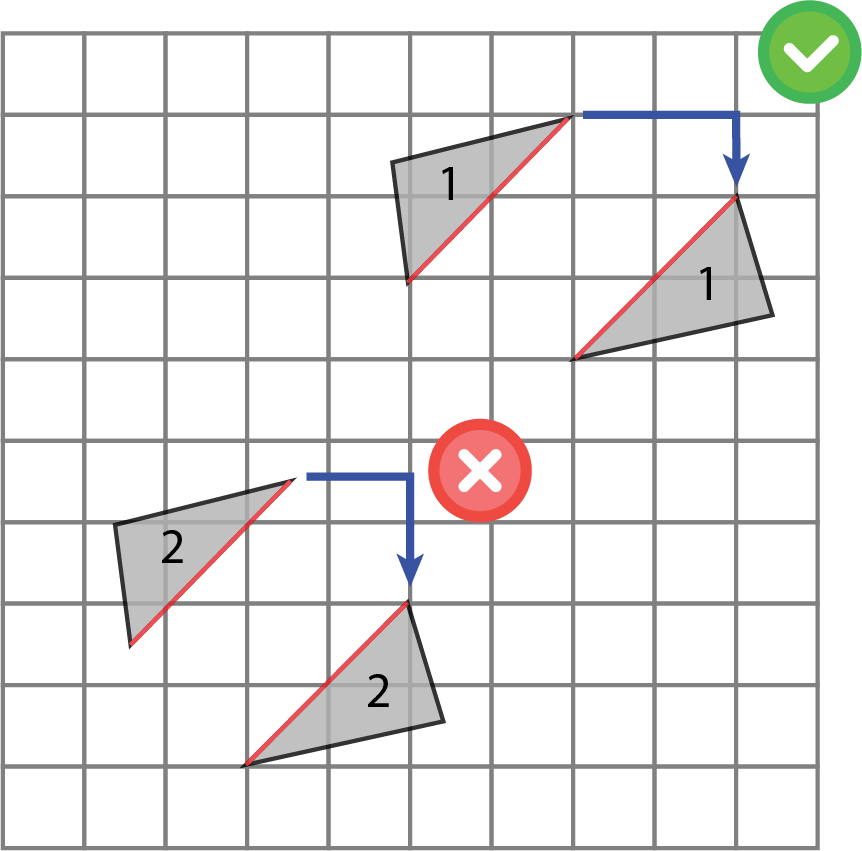
\includegraphics[width=9cm]{figures/seamless/translation.png}
\caption[The Translation Requirement]{The transition function $g_{ij}$, described by equation \ref{transition_g_ij}, should impose an integer translation between the two half edges.}
\label{fig:translation_req}
\end{figure}
\begin{figure}[ht]
\centering
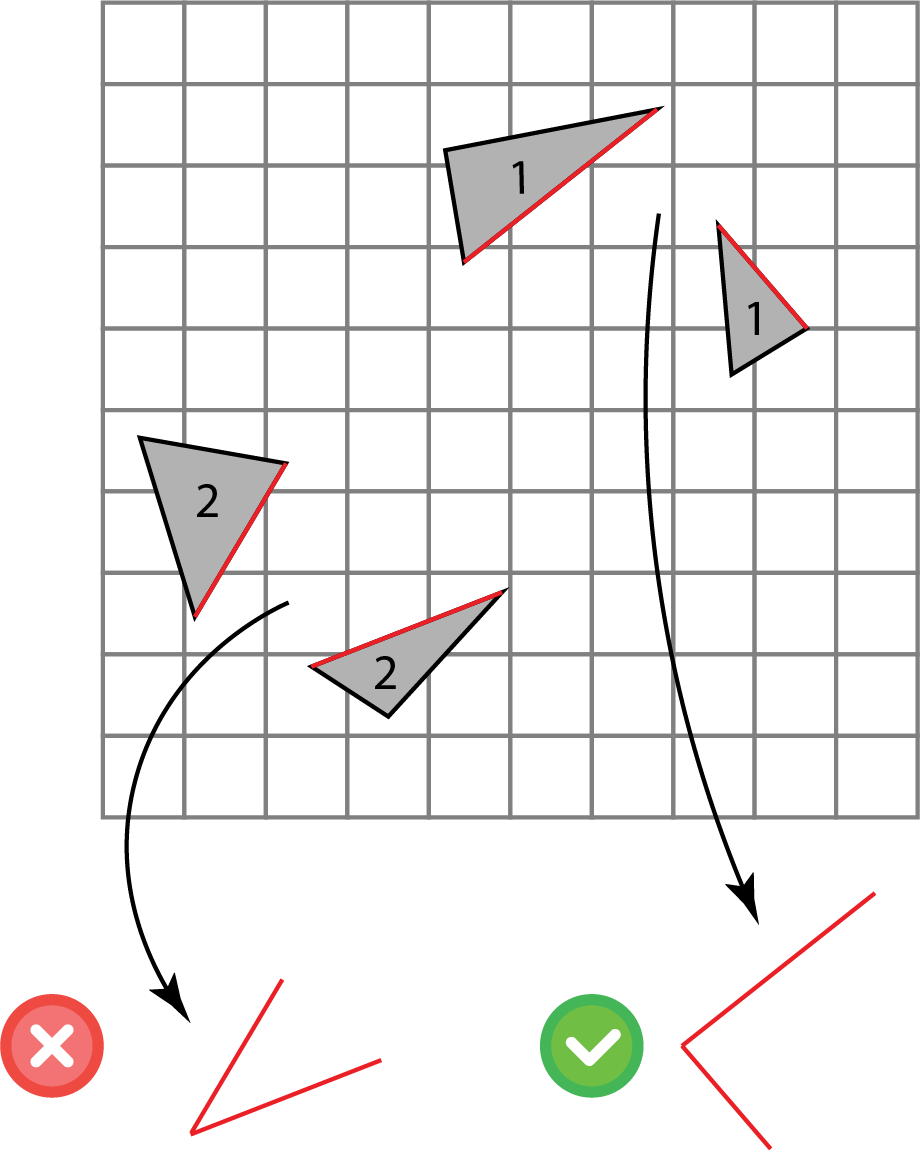
\includegraphics[width=9cm]{figures/seamless/angle.png}
\caption[The Angle Requirement]{The transition function $g_{ij}$, described by equation \ref{transition_g_ij}, should impose a $\frac{\pi}{2}k$ rotation between the two half edges.}
\label{fig:angle_req}
\end{figure}
\begin{figure}[ht]
\centering
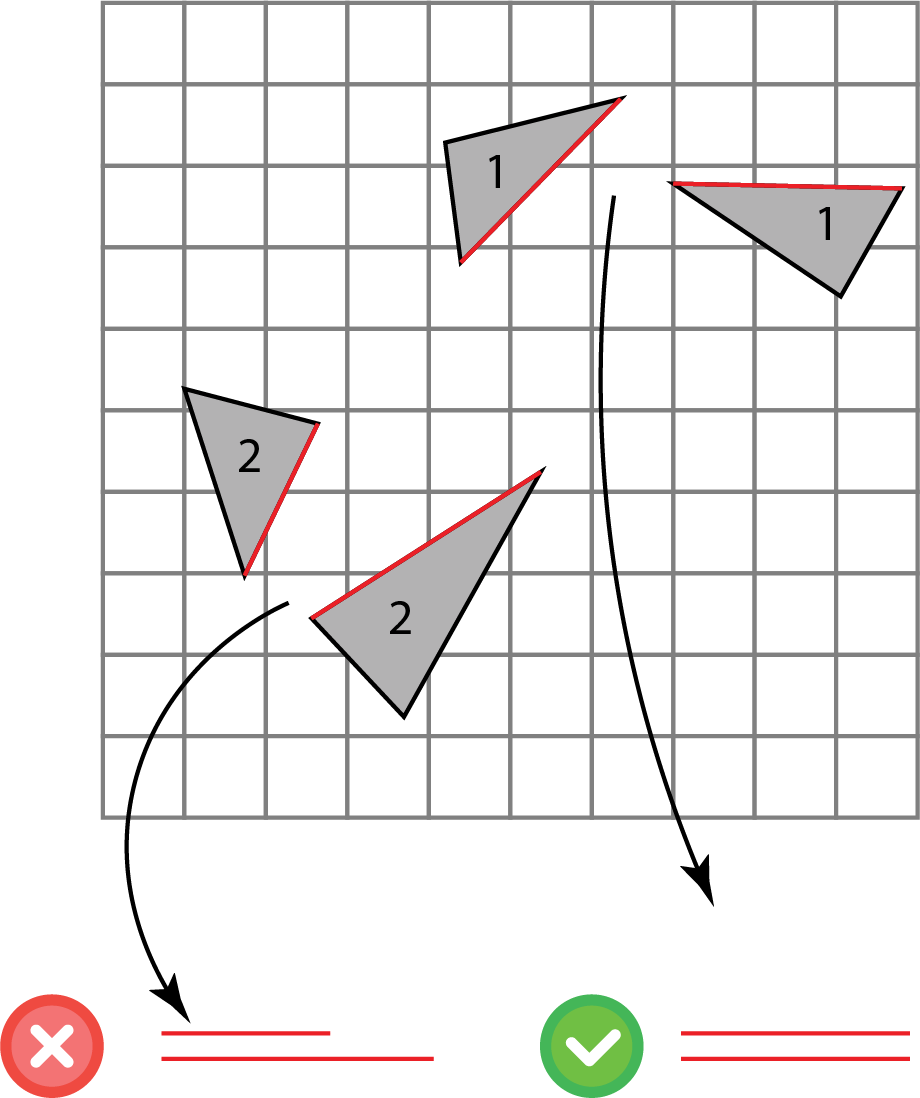
\includegraphics[width=9cm]{figures/seamless/length.png}
\caption[The Length Requirement]{The transition function $g_{ij}$, described by equation \ref{transition_g_ij}, should implicitly match the length of the two half edges.}
\label{fig:length_req}
\end{figure}
\subsection{Singular Points Condition}
\label{label:singular_points_cond}
Before we define what the singular-points condition is, we first have to define how a singular vertex is characterized on the parametrization domain. A singular-vertex (valence $\neq 4$) on the mesh's surface, will be characterized on the parametrization domain by a non-zero angular defect. The angular defect is measured by $2\pi - \sum_{i=1}^k \theta_i$ and $\pi - \sum_{i=1}^k \theta_i$ for interior and boundary surface vertices, respectively, where $k$ is the number of twin-vertices on the the parametrization domain that correspond to the singular-vertex on the mesh's surface, and $\theta_i$ is the angle adjacent to twin-vertex $v_i$.
Having the right definitions, the singular-points condition require that all twin-vertices of singular points will be located on integer locations. Formally, given the set $V$ of all twin-vertices on the domain the that correspond to the a singular vertex on the mesh's surface, we require that:
\begin{equation}\label{eq:singular_points_cond}
\begin{split}
\forall u \in V: u \in \mathbb{Z}^2
\end{split}
\end{equation}
Figure \ref{fig:singular_points_req} demonstrate this condition visually.
\begin{figure}[ht]
\centering
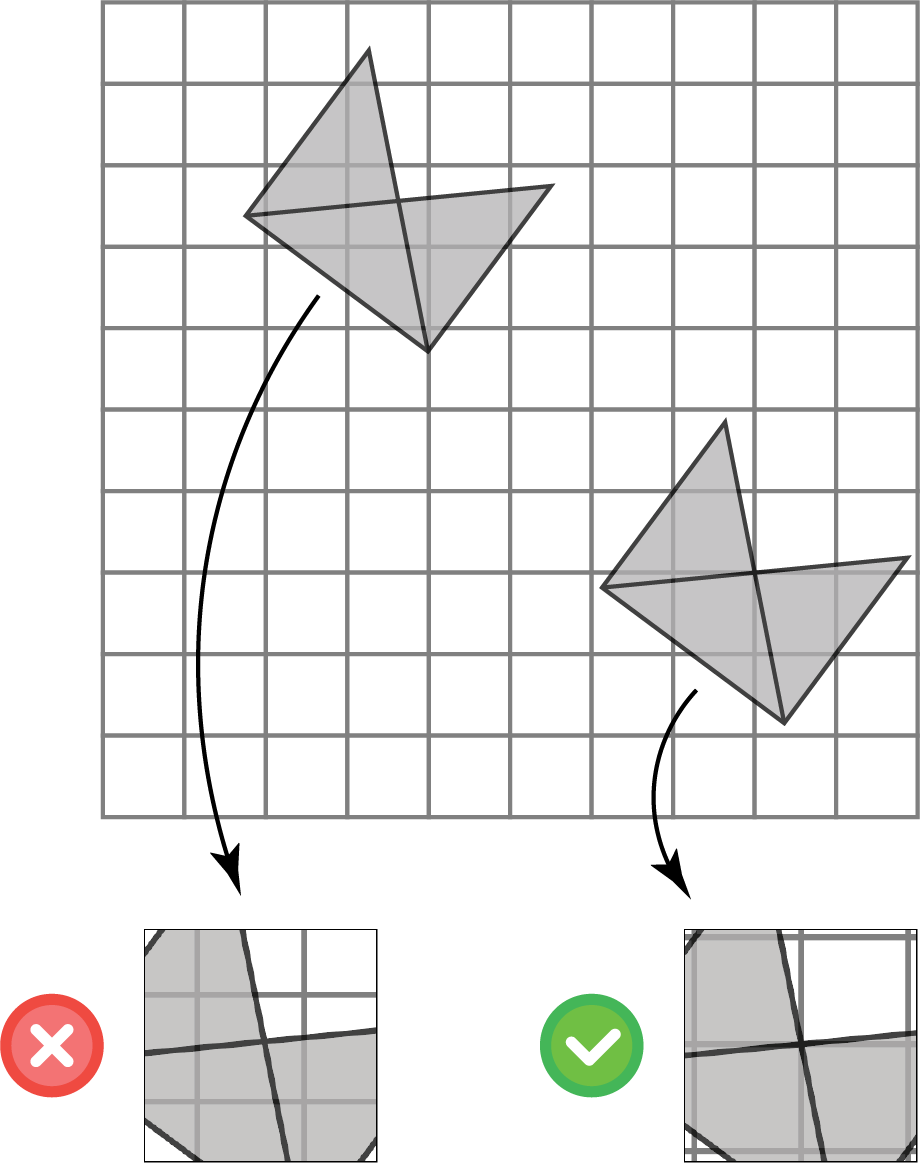
\includegraphics[width=9cm]{figures/singular_points/singularity.png}
\caption[The Singular Points Requirement]{Domain vertices that correspond to the same singular point should be positioned at a integer locations (grid points). In this illustration, the angular defect is $\frac{\pi}{2}$.}
\label{fig:singular_points_req}
\end{figure}
\subsection{Consistent Orientation Condition}
\label{label:consistent_otrientation_cond}
All triangles on the parameterization domain should have the same orientation. In other words, the transition function should not allow triangle flips. Figure \ref{fig:orientation_req} demonstrate this condition visually.
\begin{figure}[ht]
\centering
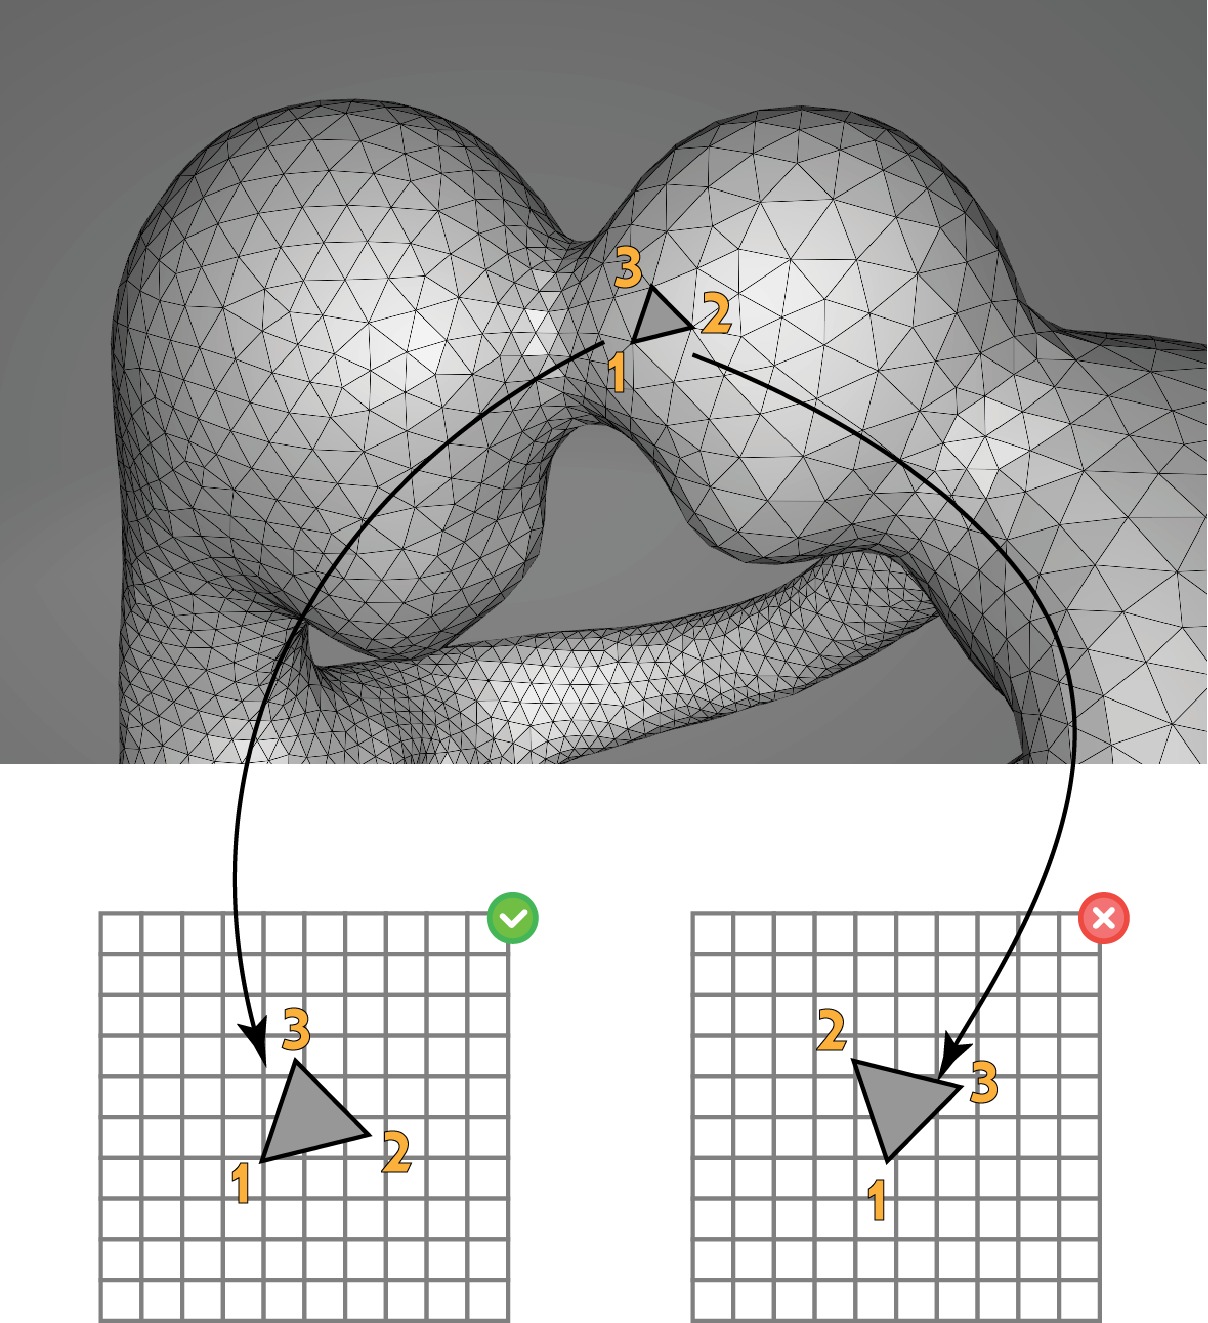
\includegraphics[width=9cm]{figures/orientation/orientation.png}
\caption[The Orientation Requirement]{The left triangle follows the same counter clockwise orientation as its image on the mesh's surface. On the other hand, the vertices of the triangle on the right follows a clockwise orientation.}
\label{fig:orientation_req}
\end{figure}
\section{Quad Distortion}
\label{label:quad_distortion_cond}
The fulfilment of the integer-grid maps conditions do guarantee that the isolines of the 2D Cartesian grid forms a valid quad-mesh on the 3D mesh's surface, however, we do have to consider at what cost. There are many possible integer-grid maps that transform a given triangle-mesh into a quad-mesh. Amongst them, we would like to pick the one that satisfies our desired set of additional requirements. In order to meet this desiderata, we have to pay with shape distortion of the triangles that make up the parametrization domain. Ultimately, we would like to find a map that fits our needs and minimizes the triangles distortion, since a distorted triangle renders a distorted isoline on the input mesh surface, which eventually affects the quality of the extracted quads that correspond to that triangle. Therefore, in addition to the integer-grid maps conditions, we add an additional implicit core requirement, which demands to find a mapping that minimizes triangle distortion. Figure \ref{fig:distortion_req} demonstrate this requirement visually.
\begin{figure}[ht]
\centering
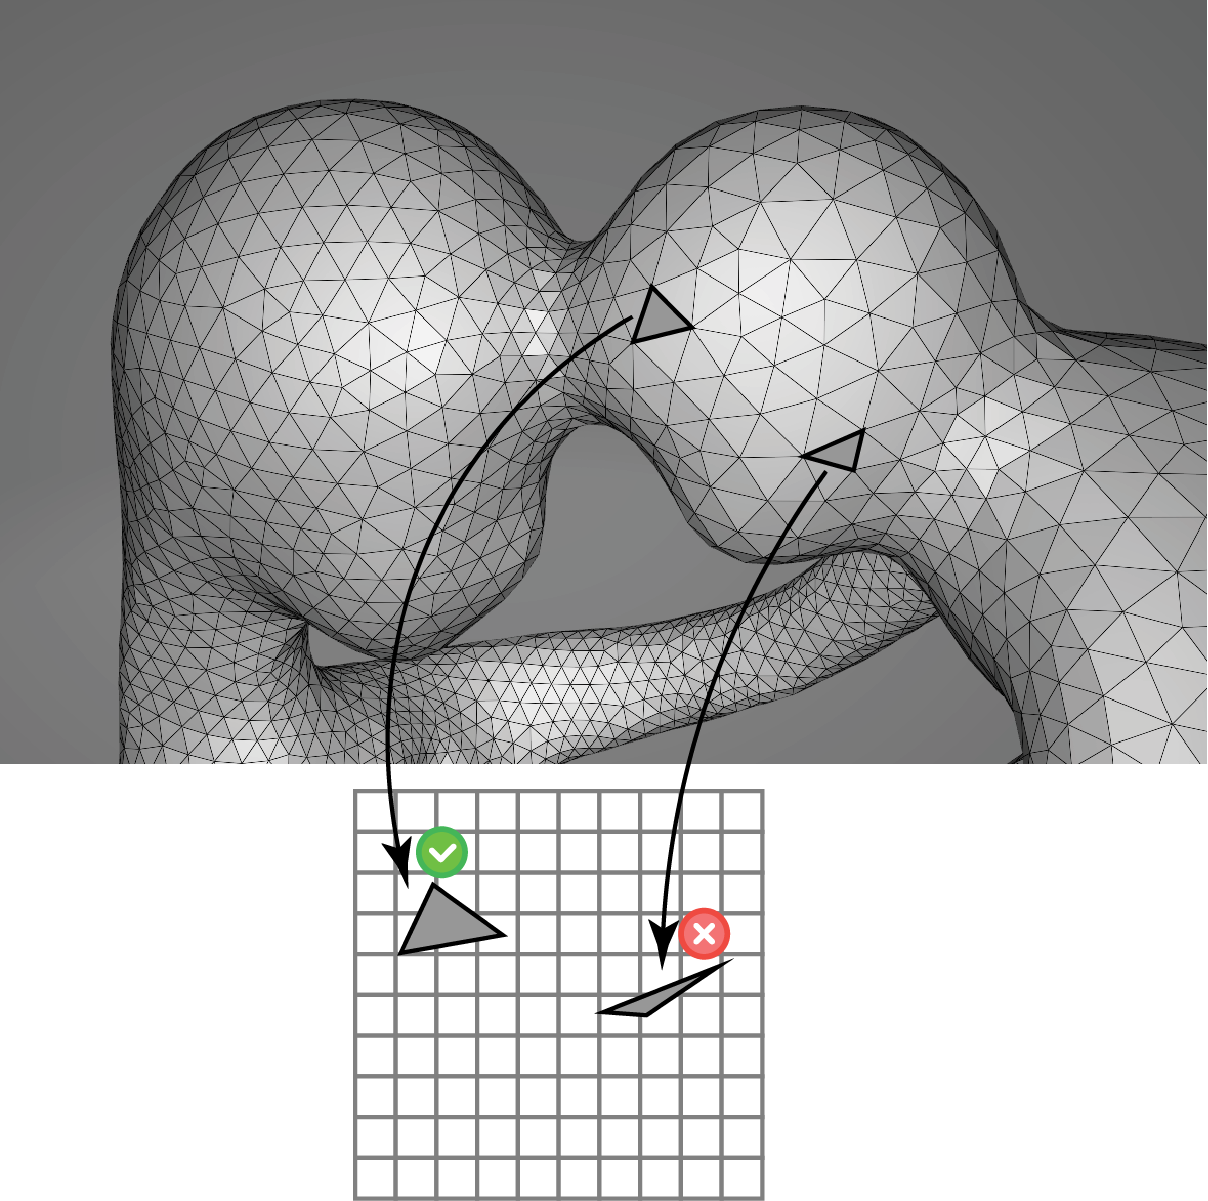
\includegraphics[width=9cm]{figures/distortion/distortion.png}
\caption[The Orientation Requirement]{The left triangle has a little shape distortion compared with its original version on the input-mesh's surface, in contrast with the right triangle, which clearly express a high shape distortion compared with its original version}
\label{fig:distortion_req}
\end{figure}
\section{Smooth Objective Functions}
In this section, we present our smooth objective function formulations for Conditions \ref{label:seamless_cond}, \ref{label:singular_points_cond}, \ref{label:consistent_otrientation_cond} and requirement \ref{label:quad_distortion_cond} presented in the previous sections. Please note, in the following sections and subsections below, we denote by $\mathrm{x}\left(v\right)$, $\mathrm{y}\left(v\right)$ the $x$ and $y$ domain coordinates of a given domain vertex $v$.
\subsection{The Seamless Condition's Objective Functions}
The seamless condition can be expressed by three smooth objective (penalty) functions $P_{angle}$, $P_{length}$ and $P_{translation}$, that penalize violations in angle, length and translation, respectively, for a given pair of half-edges. In the following three paragraphs, we define those tree penalty functions, and assume we're given two half-edges, in the parametrization domain, denoted by $e_i = \left(v_i^1,v_i^2\right)$ and $e_j = \left(v_j^1,v_j^2\right)$, where for for $k \in \left\{i,j\right\}$, $v_k^1$ and $v_k^2$ are the two domain vertices that constitutes half-edge $k$, and for $k \in \left\{1,2\right\}$, $v_i^k$ and $v_j^k$ are twin-vertices.
\paragraph{Angle Penalty}
We define $P_{angle}$ as follows:
\begin{equation}\label{eq:angle_penalty}
\begin{split}
P_{angle}\left(e_i,e_j\right) = \mathrm{sin} \bigg( 4\Big(\theta\left(e_i\right) - \theta\left(e_j\right)\Big) - \frac{\pi}{2}\bigg) + 1
\end{split}
\end{equation}
Where $\theta\left(e_k\right) = \mathrm{atan2}\Big(\mathrm{y}\left(v_k^2\right) - \mathrm{y}\left(v_k^1\right), \mathrm{x}\left(v_k^2\right) - \mathrm{x}\left(v_k^1\right)\Big)$ is the angle formed by half-edge $k$ with the positive \emph{x-axis} direction, when treated as a vector based at $v_k^1$ and heading $v_k^2$, for $k \in \left\{i,j\right\}$. Therefore, the expression $\theta\left(e^i\right) - \theta\left(e^j\right)$ yields the signed angle between the two half-edges. Figure \ref{fig:angle_penalty} shows a plot of the angle penalty function for a range of $\theta$ values. It is easy to see that the angle penalty is minimized when the angle discrepancy between the two half-edges is an integer multiple of $\frac{\pi}{2}$, as required by the seamless condition. Please note, equation \ref{eq:angle_penalty} yields only non-negative values due to the introduction of the $+1$ term.
\begin{figure}[ht]
\centering
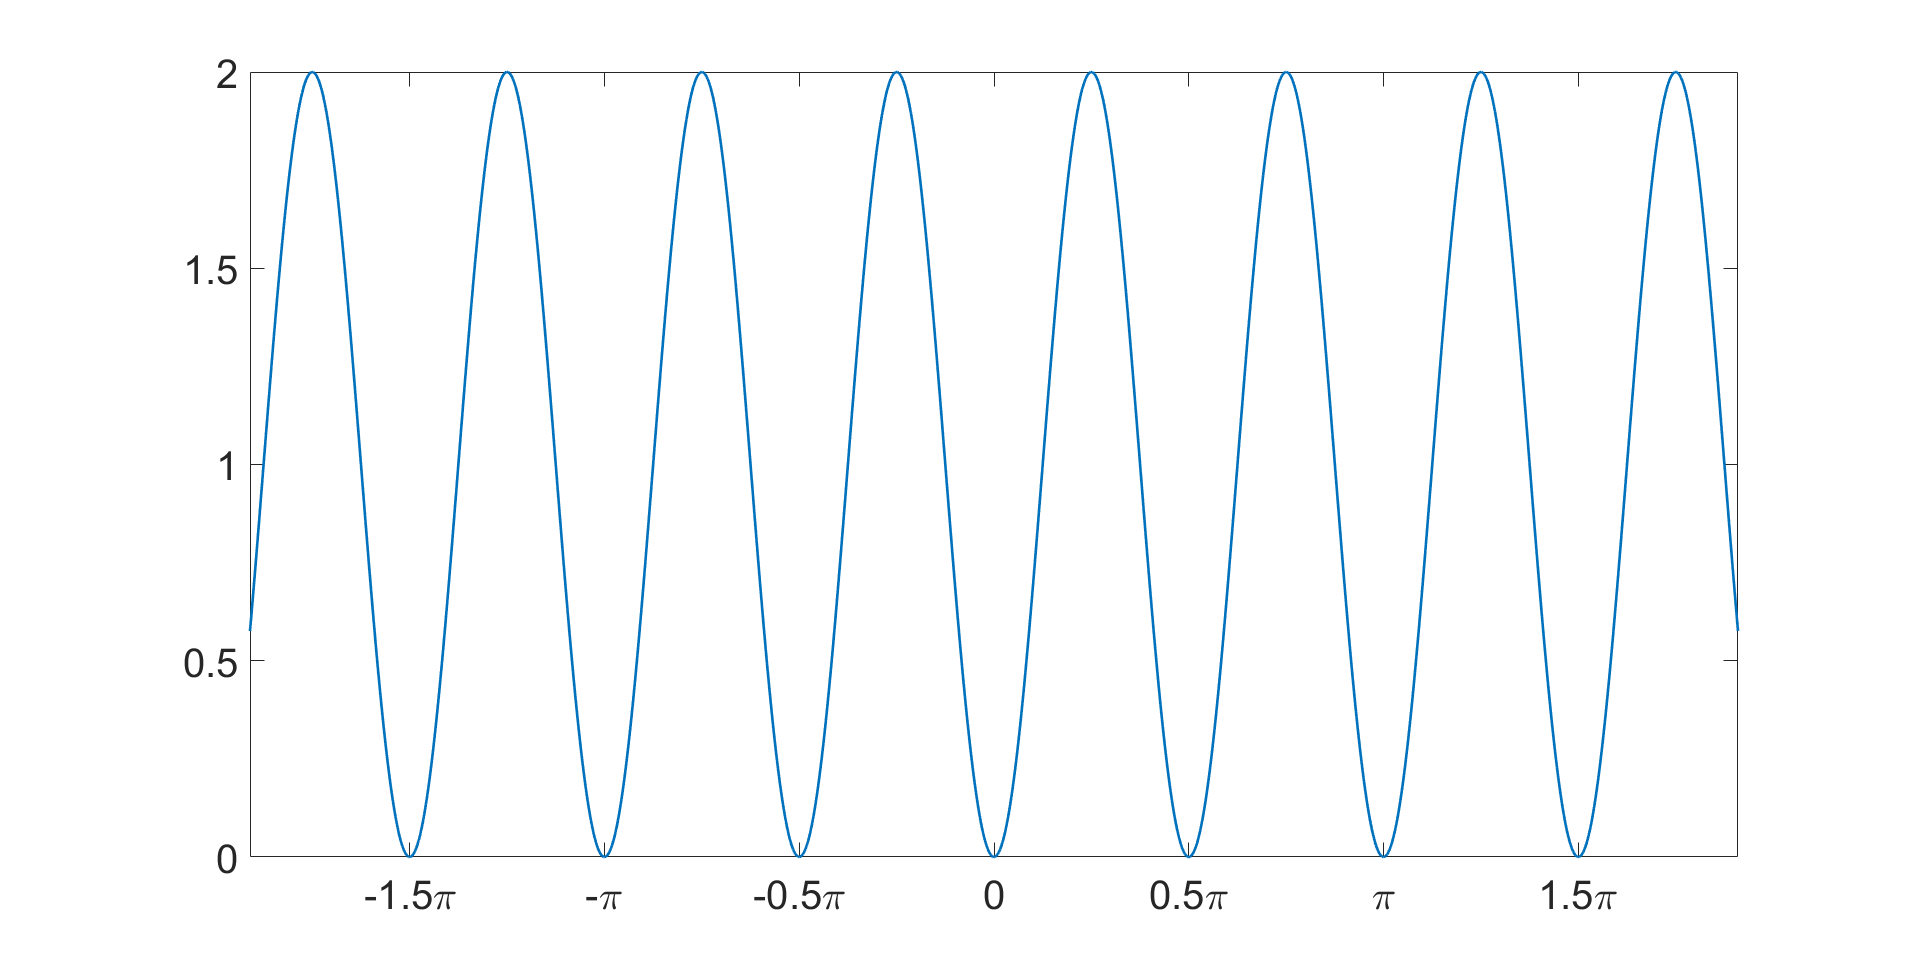
\includegraphics[width=15cm]{figures/seamless/angle_penalty_function.png}
\caption[The Angle Penalty Function]{A plot of the angle penalty function for a range of $\theta$ values. The penalty is zero for values of integer multiples of $\frac{\pi}{2}$, which represent a $\frac{\pi}{2}k$ rotation between the two half-edges, for $k \in \mathbb{N}$.}
\label{fig:angle_penalty}
\end{figure}
\paragraph{Length Penalty}
We define the length penalty function $P_{length}$ as follows:
\begin{equation}\label{length_penalty}
\begin{split}
P_{length}\left(e_i,e_j\right) = \left(\norm{e_i}_2^2 - \norm{e_j}_2^2\right)^2
\end{split}
\end{equation}
The length penalty measures the Euclidean length discrepancy between the two half-edges. It is a non-convex function (However, its Hessian is positive semi-definite almost everywhere) with multiple global minimum points associated with the function value of $0$. Therefore, It is easy to see that the length penalty is minimized when the length discrepancy between the two half-edges is absolutely zero, as required by the seamless condition. Figure \ref{fig:length_penalty} shows a plots of the length penalty function for a range of $\norm{e_i}_2^2$ and $\norm{e_j}_2^2$ values.
\begin{figure}[ht]
\centering
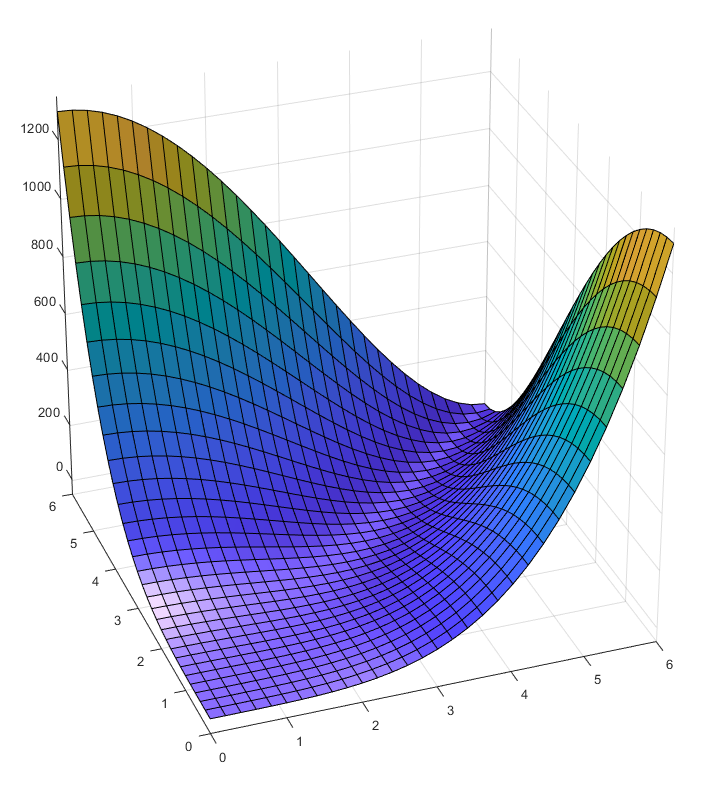
\includegraphics[width=12cm]{figures/seamless/length_penalty_function.png}
\caption[The Length Penalty Function]{A plot of the length penalty function. The penalty is zero along the $x=y$ line on the domain, where the lengths of the two half-edges are equal.}
\label{fig:length_penalty}
\end{figure}
% The length penalty measures the Euclidean length discrepancy between the two half-edges. It is a convex function (its Hessian is positive semi-definite) with multiple global minimum points associated with the function value of $0$. Therefore, It is easy to see that the length penalty is minimized when the length discrepancy between the two half-edges is absolutely zero, as required by the seamless condition.
\paragraph{Translation Penalty}
We define the translation penalty function $P_{translation}$ as follows:
\begin{equation}\label{eq:translation_penalty}
\begin{split}
P_{translation}\left(e_i,e_j\right) = \mathrm{sin} \Big( 2\pi\cdot\Delta_x\big(e_i,e_j\big) - \frac{\pi}{2}\Big) + \mathrm{sin} \Big( 2\pi\cdot\Delta_y\big(e_i,e_j\big) - \frac{\pi}{2}\Big) + 2
\end{split}
\end{equation}
Where $\Delta_x\big(e_i,e_j\big) = \mathrm{x}\left(v_i^1\right) - \mathrm{x}\left(v_j^1\right)$ and $\Delta_y\big(e_i,e_j\big) = \mathrm{y}\left(v_i^1\right) - \mathrm{y}\left(v_j^1\right)$ represent the Manhattan distance between the two twin-vertices $v^i_1$ and $v^j_1$, which is also, implicitly, the Manhattan distance between the two half-edges. Since the two sine terms in equation \ref{eq:translation_penalty} achieve their minimum value only for integer $\Delta_x$ and $\Delta_y$, it means that the function penalize non-integer Manhattan distances. Therefore, it is easy to see that the translation penalty is minimized when the two twin-vertices are integer distance apart, as required by the seamless condition. Figure \ref{fig:translation_penalty} shows a plot of the translation penalty function for a range of $\Delta_x$ and $\Delta_y$ values. Please note, equation \ref{eq:translation_penalty} yields only non-negative values due to the introduction of the $+2$ term.
\begin{figure}[ht]
\centering
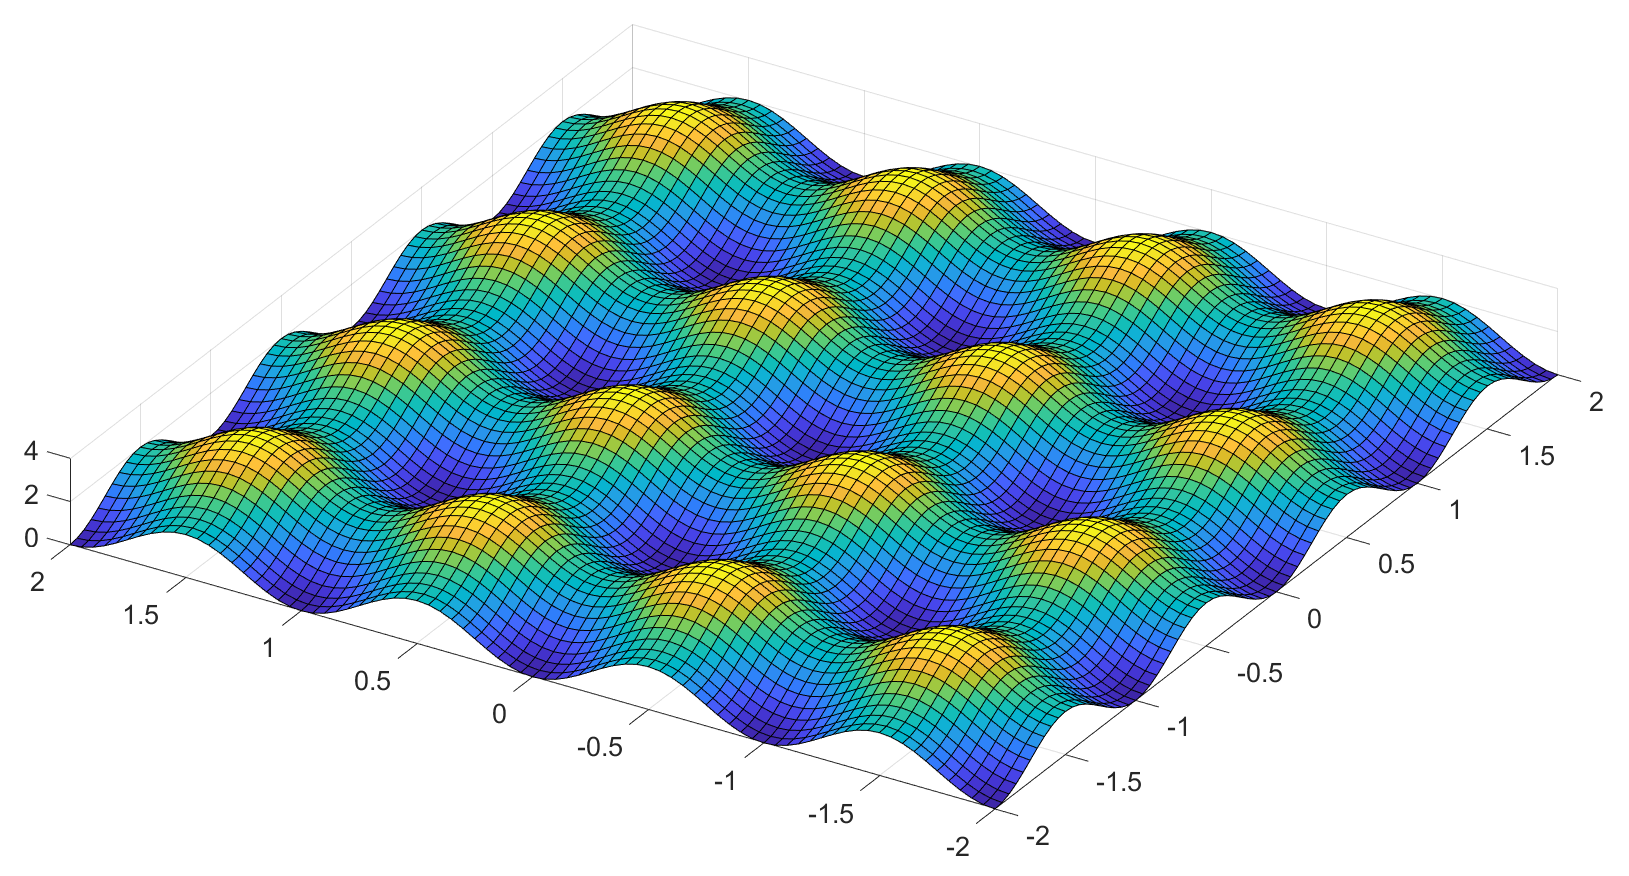
\includegraphics[width=15cm]{figures/seamless/translation_penalty_function.png}
\caption[The Translation Penalty Function]{A plot of the translation penalty function for a range of values on the domain given by $\left[-2:2, -2:2\right]$. As can be seen, global minimum points are located at integer locations, which represent integer translations.}
\label{fig:translation_penalty}
\end{figure}
\subsection{The Singular-Points Condition's Objective Function}
The singular-points penalty function is applied on groups of twin-vertices on the parametrization domain, with non-zero angular defect (as defined in subsection \ref{label:singular_points_cond}). Given a group $V$ of twin-vertices that correspond to a singular point, the singular-points penalty function applied on that group is defined as follows:
\begin{equation}\label{eq:singular_points_penalty}
\begin{split}
P_{singular}\left(V\right) = \sum_{u \in V} \bigg( \mathrm{sin} \Big( 2\pi\cdot\mathrm{x}\big(u\big) - \frac{\pi}{2}\Big) + \mathrm{sin} \Big( 2\pi\cdot\mathrm{y}\big(u\big) - \frac{\pi}{2}\Big) + 2 \bigg)
\end{split}
\end{equation}
Where $\mathrm{x}\big(u\big)$ and $\mathrm{y}\big(u\big)$ represent the domain coordinates of a twin-vertex in $V$. Since the two sine terms in equation \ref{eq:singular_points_penalty} achieve their minimum value only for integer $\mathrm{x}\big(u\big)$ and $\mathrm{y}\big(u\big)$, it means that it penalize non-integer locations of singular twin-vertices. Therefore, it is easy to see that the translation penalty is minimized when \textbf{all} twin-vertices in $V$ are located on integer locations, as required by the singular-points condition. Please note, equation \ref{eq:singular_points_penalty} yields only non-negative values due to the introduction of the $+1$ term for each sine term. Figure \ref{fig:singular_points_penalty_sine_term} shows a plot of a single sine term from the singular-points penalty function for a range of $\mathrm{x}$ (or $\mathrm{y}$) values. Figure \ref{fig:singular_points_penalty_minimum} illustrates an example where the penalty function converge to a local minimum, where all twin-vertices located at grid-point locations.
\begin{figure}[ht]
\centering
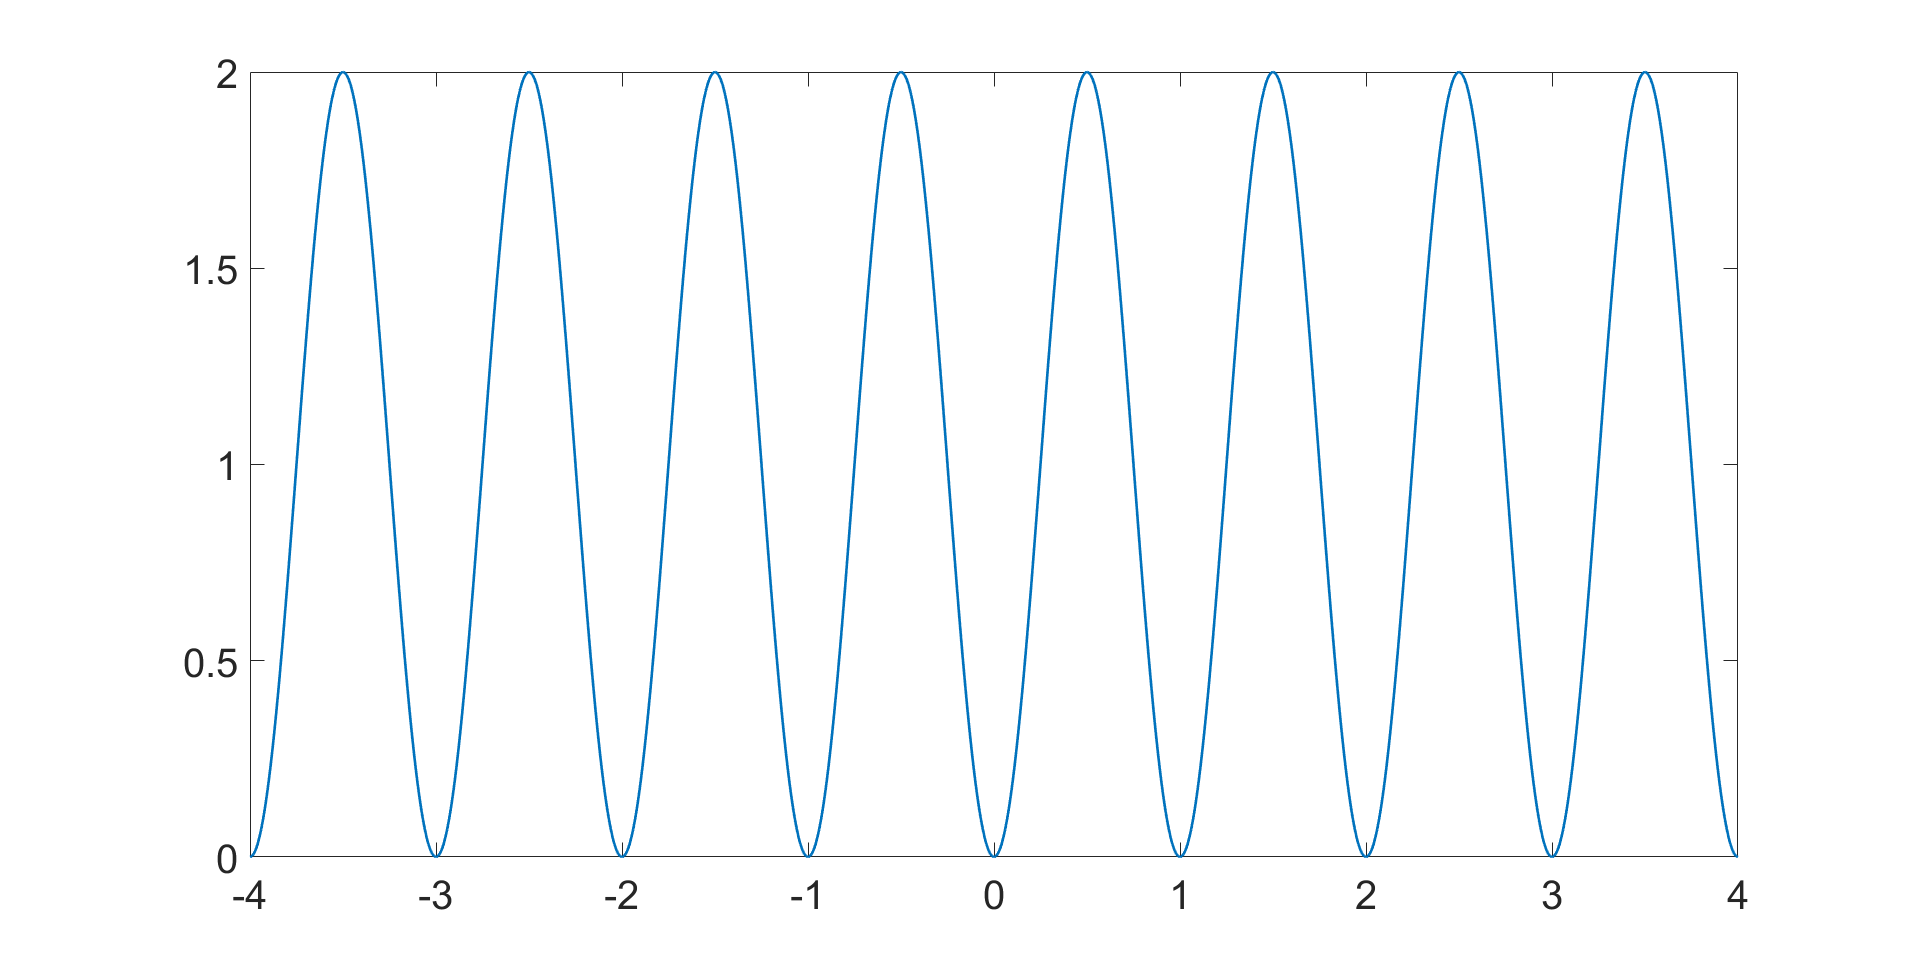
\includegraphics[width=16cm]{figures/singular_points/singular_points_penalty_function_sine_term.png}
\caption[The Singular-Points Penalty Function (Single Sine Term)]{A plot of a single sine term of the singular-points penalty function for a range of $\mathrm{x}$ (or $\mathrm{y}$). As can be seen, global minimum points are located at integer locations, which represent integer grid coordinates.}
\label{fig:singular_points_penalty_sine_term}
\end{figure}
\begin{figure}[ht]
\centering
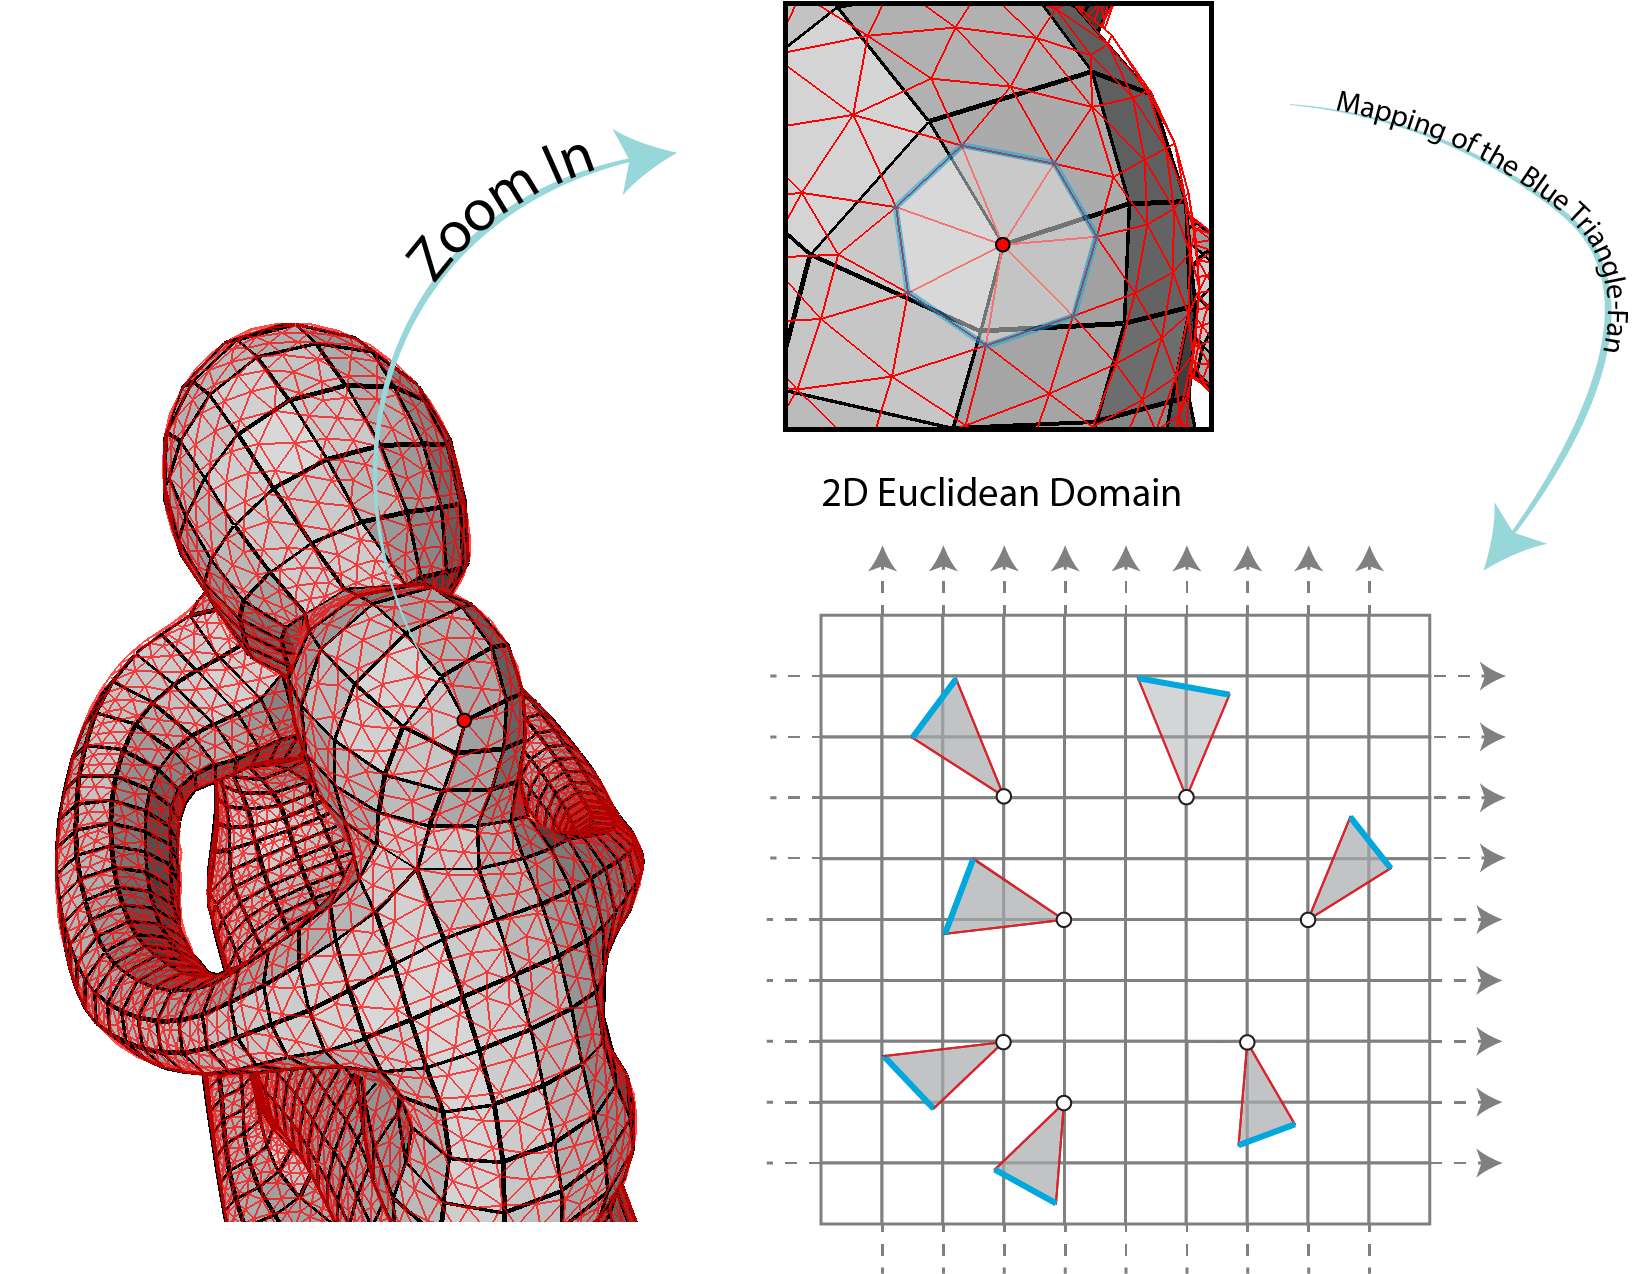
\includegraphics[width=16cm]{figures/singular_points/singular_points_penalty_function_minimum.png}
\caption[Singular-Points Penalty Function Global Minimum Example]{An example where the singular-points penalty function converges to a local minimum, when applied to a single singular-point. The red point on the mesh's surface represents a singular point of valence 3 (with respect to the black isolines), composed of a 7-facets blue triangle-fan. The corresponding triangle-soup on the parametrization domain satisfies the requirement that all twin-vertices of the singular-point are located on integer grid points. The sum of angles, adjacent to the group of twin-vertices, has a non-zero angular defect of $\frac{\pi}{2}$.}
\label{fig:singular_points_penalty_minimum}
\end{figure}
\subsection{The Consistent Orientation and Quad Distortion Conditions' Objective Functions}
In this subsection, we denote by $J\left(f_i\right)$ the Jacobian of the linear part of the affine mapping of triangle $f_i$ on the parametrization domain. Inspired by \cite{Smith:2015} and \cite{Poranne:Autocuts:2017}, we express both the consistent-orientation condition and the requirement to minimize triangle distortion on the domain, by the following penalty function:
\begin{equation}\label{eq:orientation_and_distortion_penalty}
\begin{split}
P_{\mathrm{dirichlet}}\left(f_i\right) = P_{\mathrm{distortion}}\left(f_i\right) + P_{\mathrm{orientation}}\left(f_i\right)
\end{split}
\end{equation}
Where the left term is given by $P_{\mathrm{distortion}}\left(f_i\right) = \norm{J\left(f_i\right)}_F^2$ , the right term is given by $P_{\mathrm{orientation}}\left(f_i\right) = \norm{J\left(f_i\right)^{-1}}_F^2$, and $\norm{\cdot}_F^2$ is the squared Frobenius norm. It is known that for $A \in \mathbb{R}_{n \times n}$, the Frobenius norm of $A$ is a function of its singular values given by $\norm{A}_F^2 = \sqrt{\sum_{i=1}^{n} \sigma_i^2}$. Therefore, since $J\left(f_i\right) \in \mathbb{R}_{2 \times 2}$, we can rewrite $P_{\mathrm{dirichlet}}$ as follows:
\begin{equation}\label{eq:orientation_and_distortion_penalty_explicit}
\begin{split}
P_{\mathrm{dirichlet}}\left(f_i\right) = \sigma^2_1 + \sigma^2_2 + \sigma^{-2}_1 +\sigma^{-2}_2
\end{split}
\end{equation}
Where $\sigma_1$ and $\sigma_2$ are the two singular values of $J\left(f_i\right)$. Given that the mapping is initialized such that $\sigma_i > 0$, the dirichlet penalty function will prevent triangle flips since $\sigma^{-2}_i \xrightarrow[\sigma_i \to 0^+]{} \infty$, for $i \in \left\{1,2\right\}$. Moreover, the dirichlet penalty function is minimized when the Jacobian induce an isometric mapping, since its global minimum is achieved at $\sigma_1 = 1$ and $\sigma_2 = 1$. Figure \ref{fig:dirichlet_penalty_function} illustrate the dirichlet penalty function for a range of $\sigma_1$ and $\sigma_2$ values.
\begin{figure}[ht]
\centering
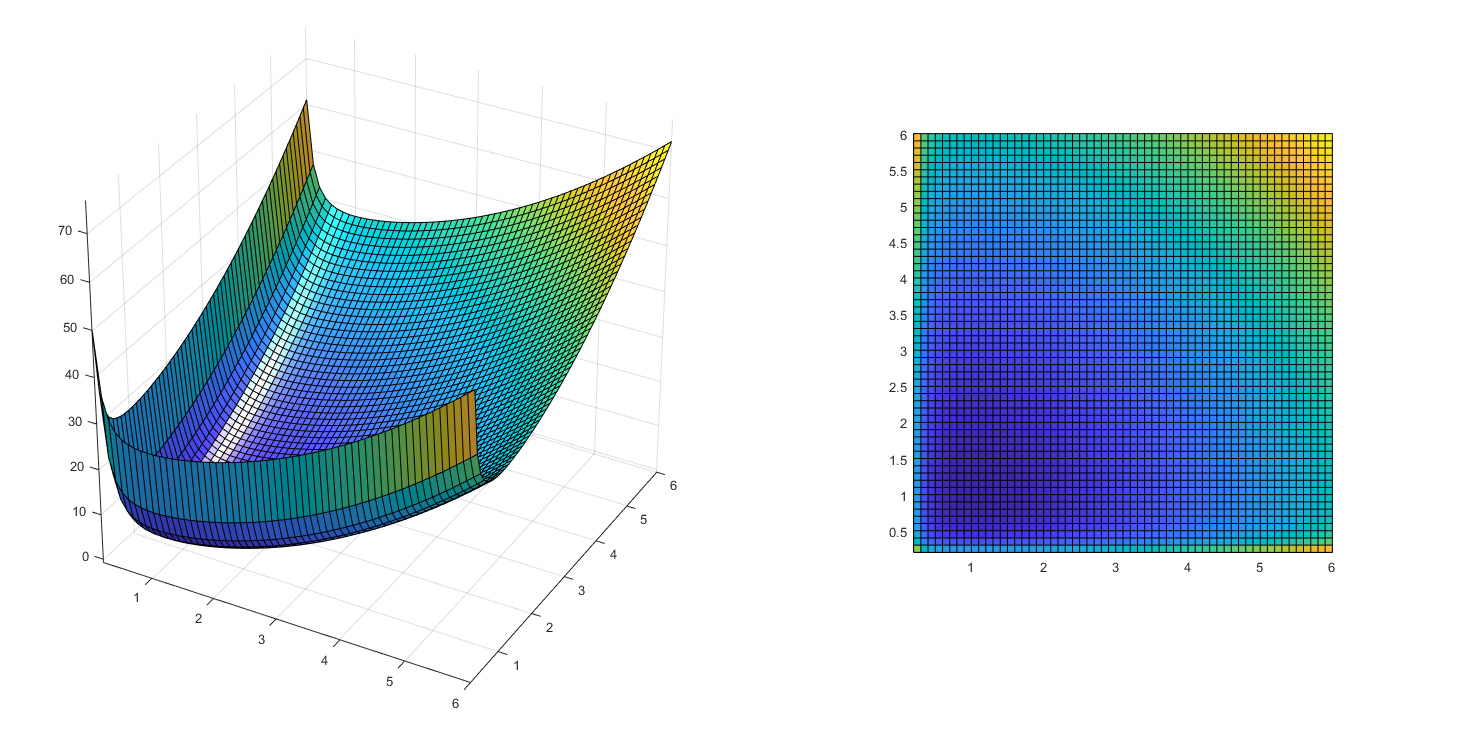
\includegraphics[width=16cm]{figures/dirichlet/symmetric_dirichlet_penalty_function.png}
\caption[The Symmetric Dirichlet Penalty Function]{On the left, a perspective view of the dirichlet penalty function is plotted. As can be seen, "walls" are formed along the positive $\sigma_1 = 0$ and $\sigma_2 = 0$ half-lines, infinitely penalizing an attempt to cross into an adjacent quadrant. On the right, a top view of the dirichlet penalty function is plotted, clearly showing that its global minimum is achieved at $\sigma_1 = 1$ and $\sigma_2 = 1$.}
\label{fig:dirichlet_penalty_function}
\end{figure}
\subsection{The Main Objective Function}
\chapter{Results}
\label{chapter:results}
In this chapter we present quadrangulations of various input triangle-meshes, produced using a simple design tool we've built to demonstrate our method. Each figure is order from left to right, and top to bottom, and include a screenshot of the system's initial state upon loading an input triangle-mesh model, and a few screen captures from different point-of-views, of the final quadrangulation result. Singular-points are highlighted in red. Each input triangle-mesh was simplified to include 600 faces.
\newpage
\section{Bunny Model}
\begin{figure}[ht]
\centering
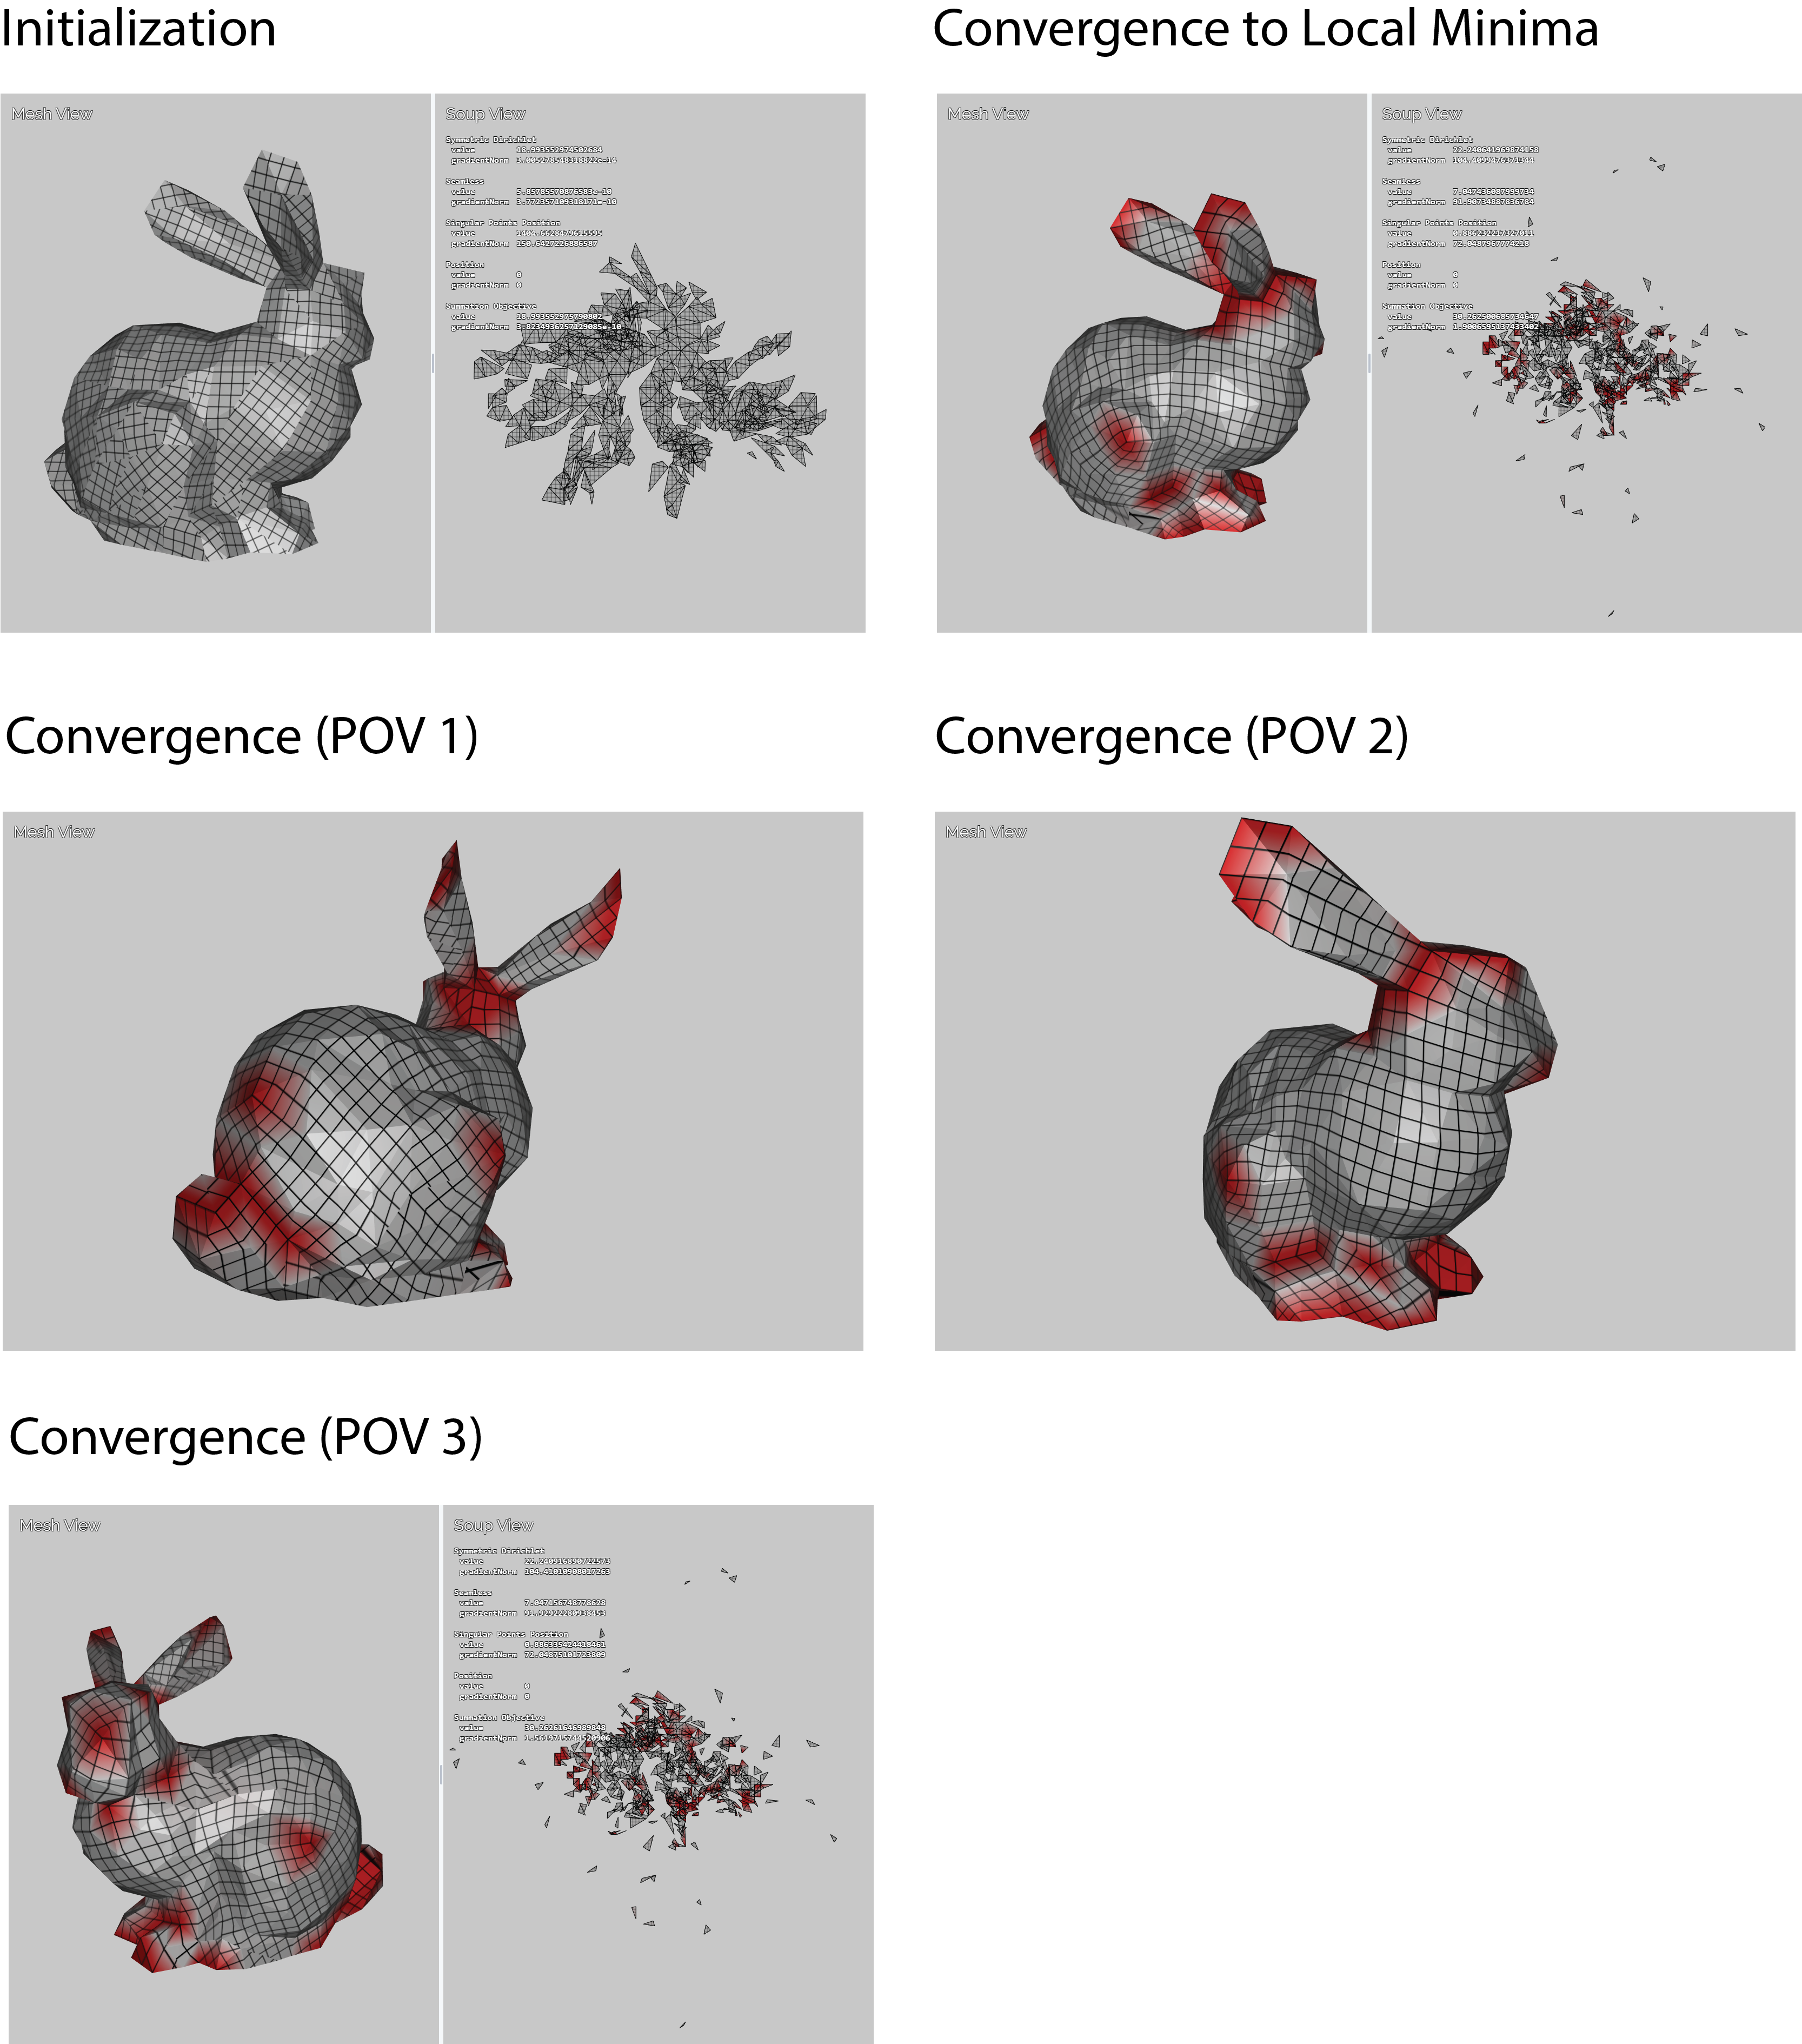
\includegraphics[width=14cm]{figures/results/bunny.png}
\caption[Bunny Model]{}
\end{figure}
\newpage
\section{Teddy Bear Model}
\begin{figure}[ht]
\centering
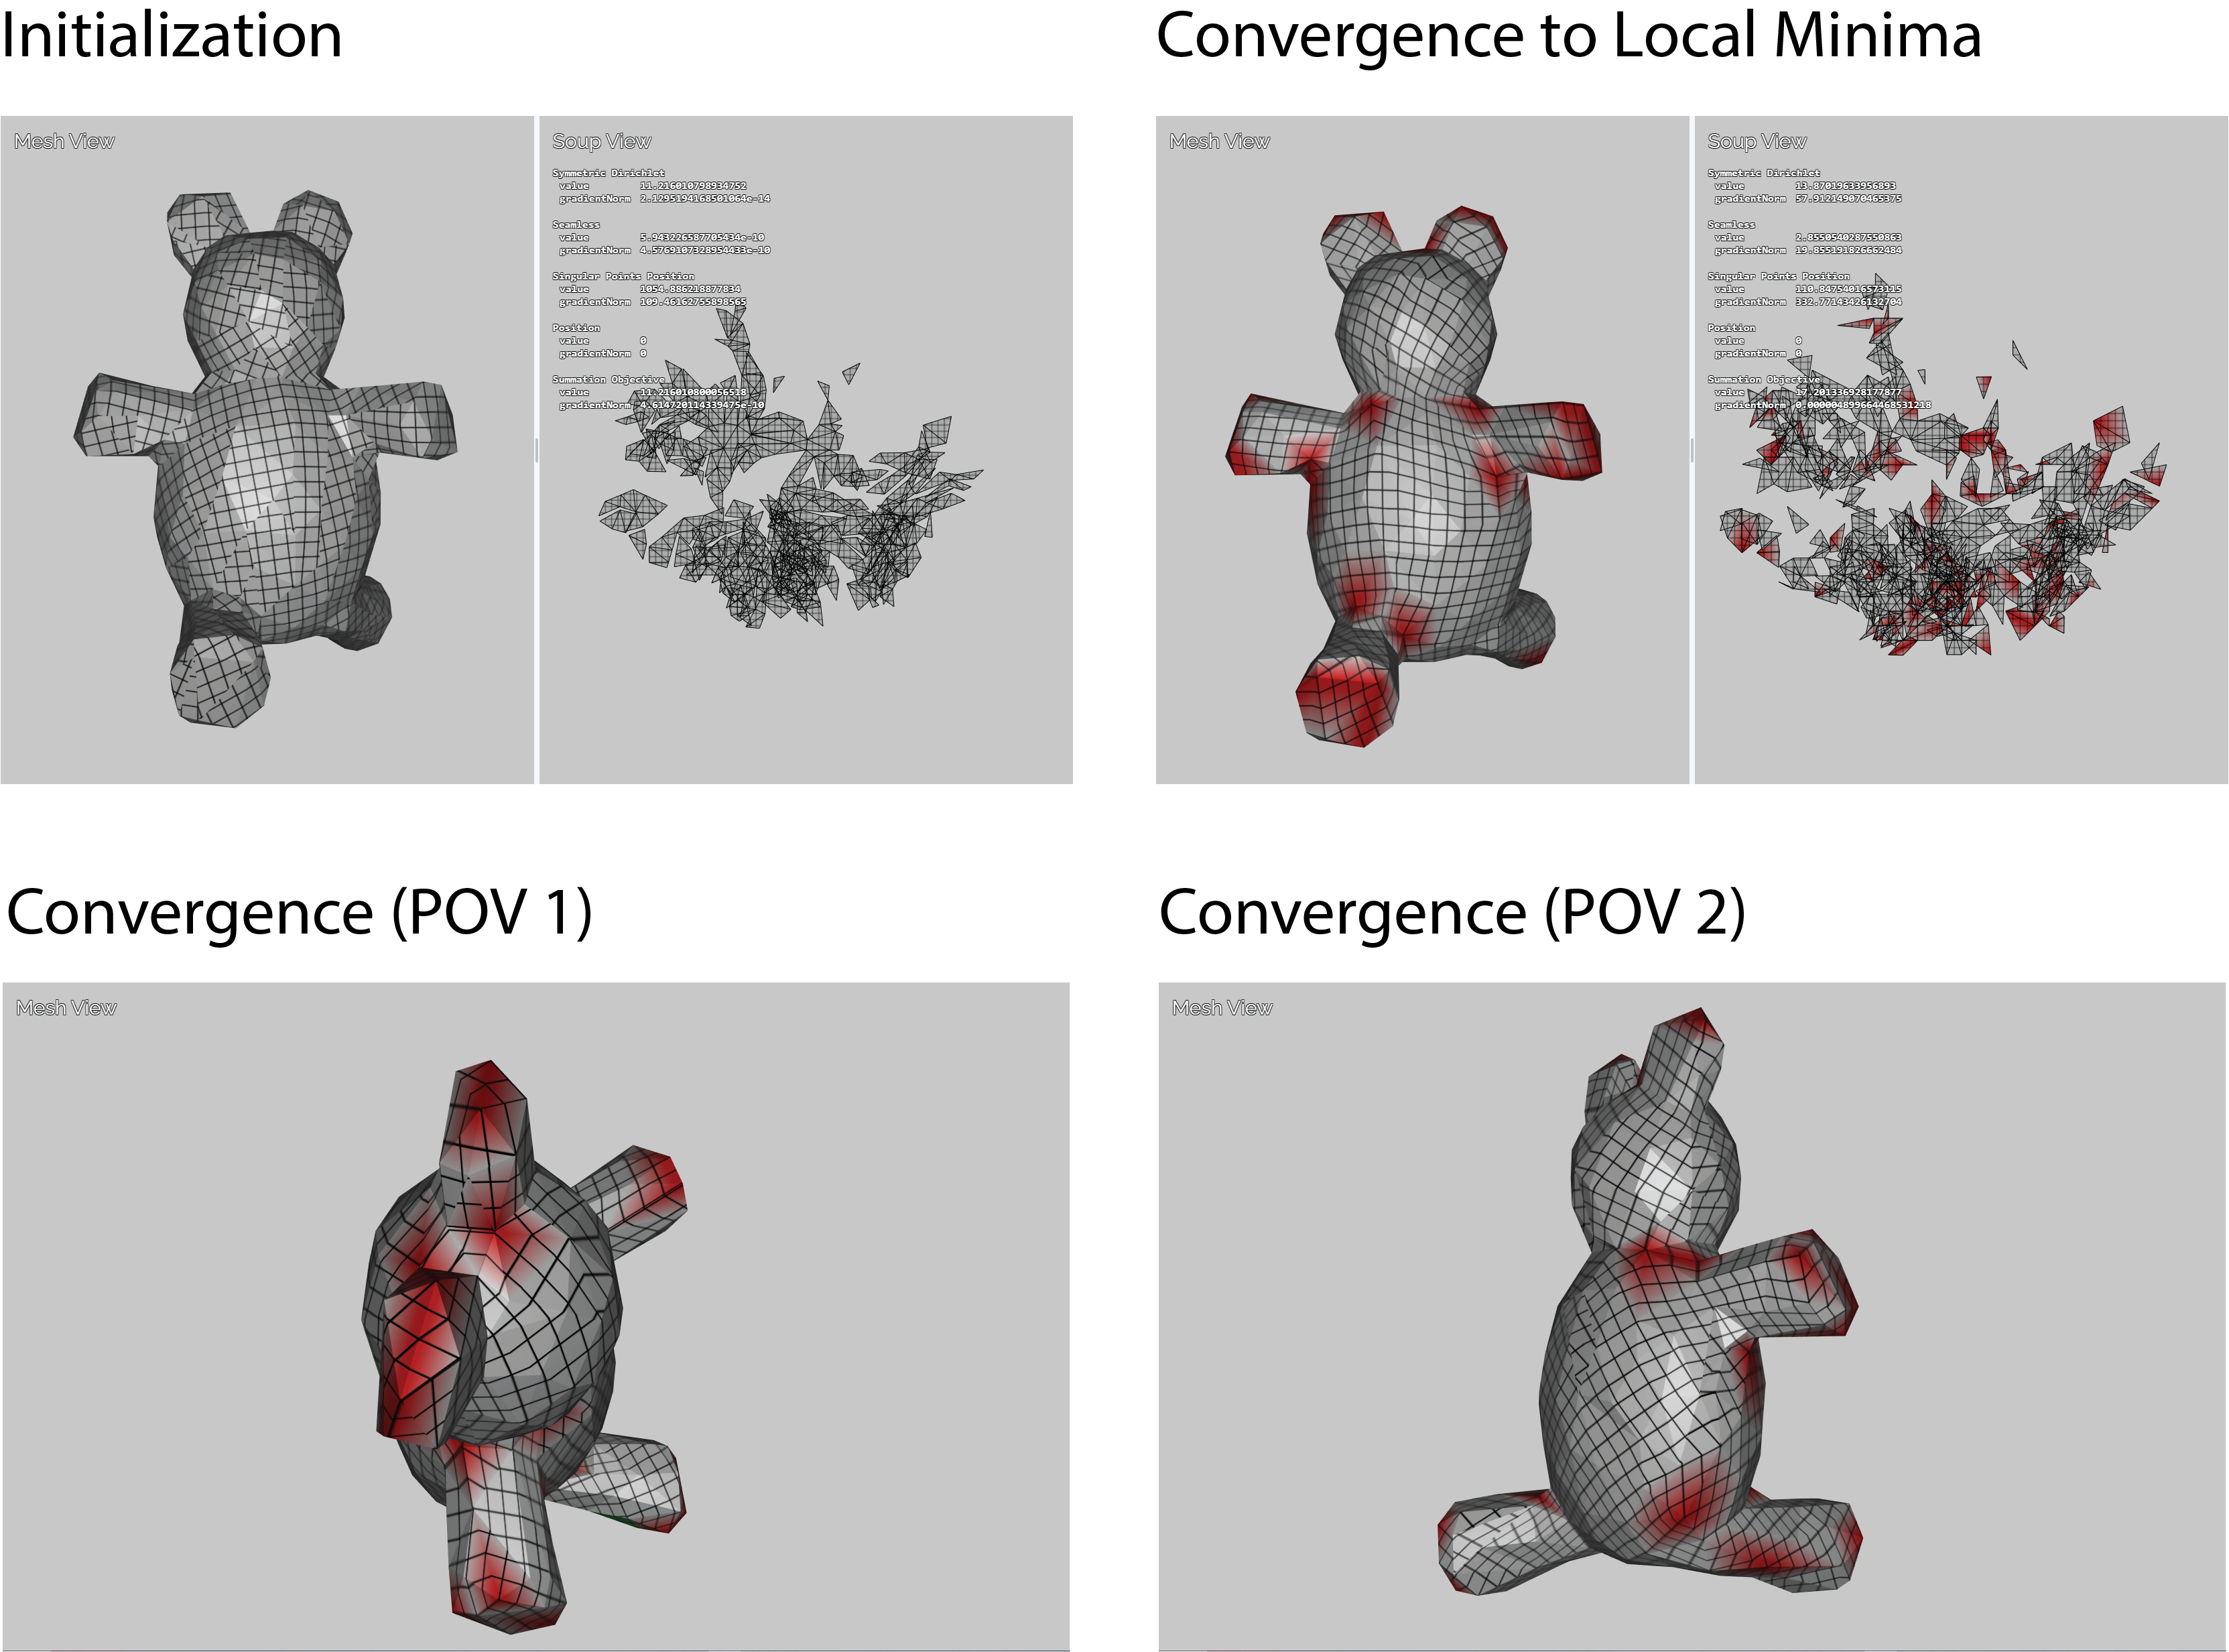
\includegraphics[width=14cm]{figures/results/teddy.png}
\caption[Teddy Bear Model]{}
\end{figure}
\newpage
\section{Kitten Model}
\begin{figure}[ht]
\centering
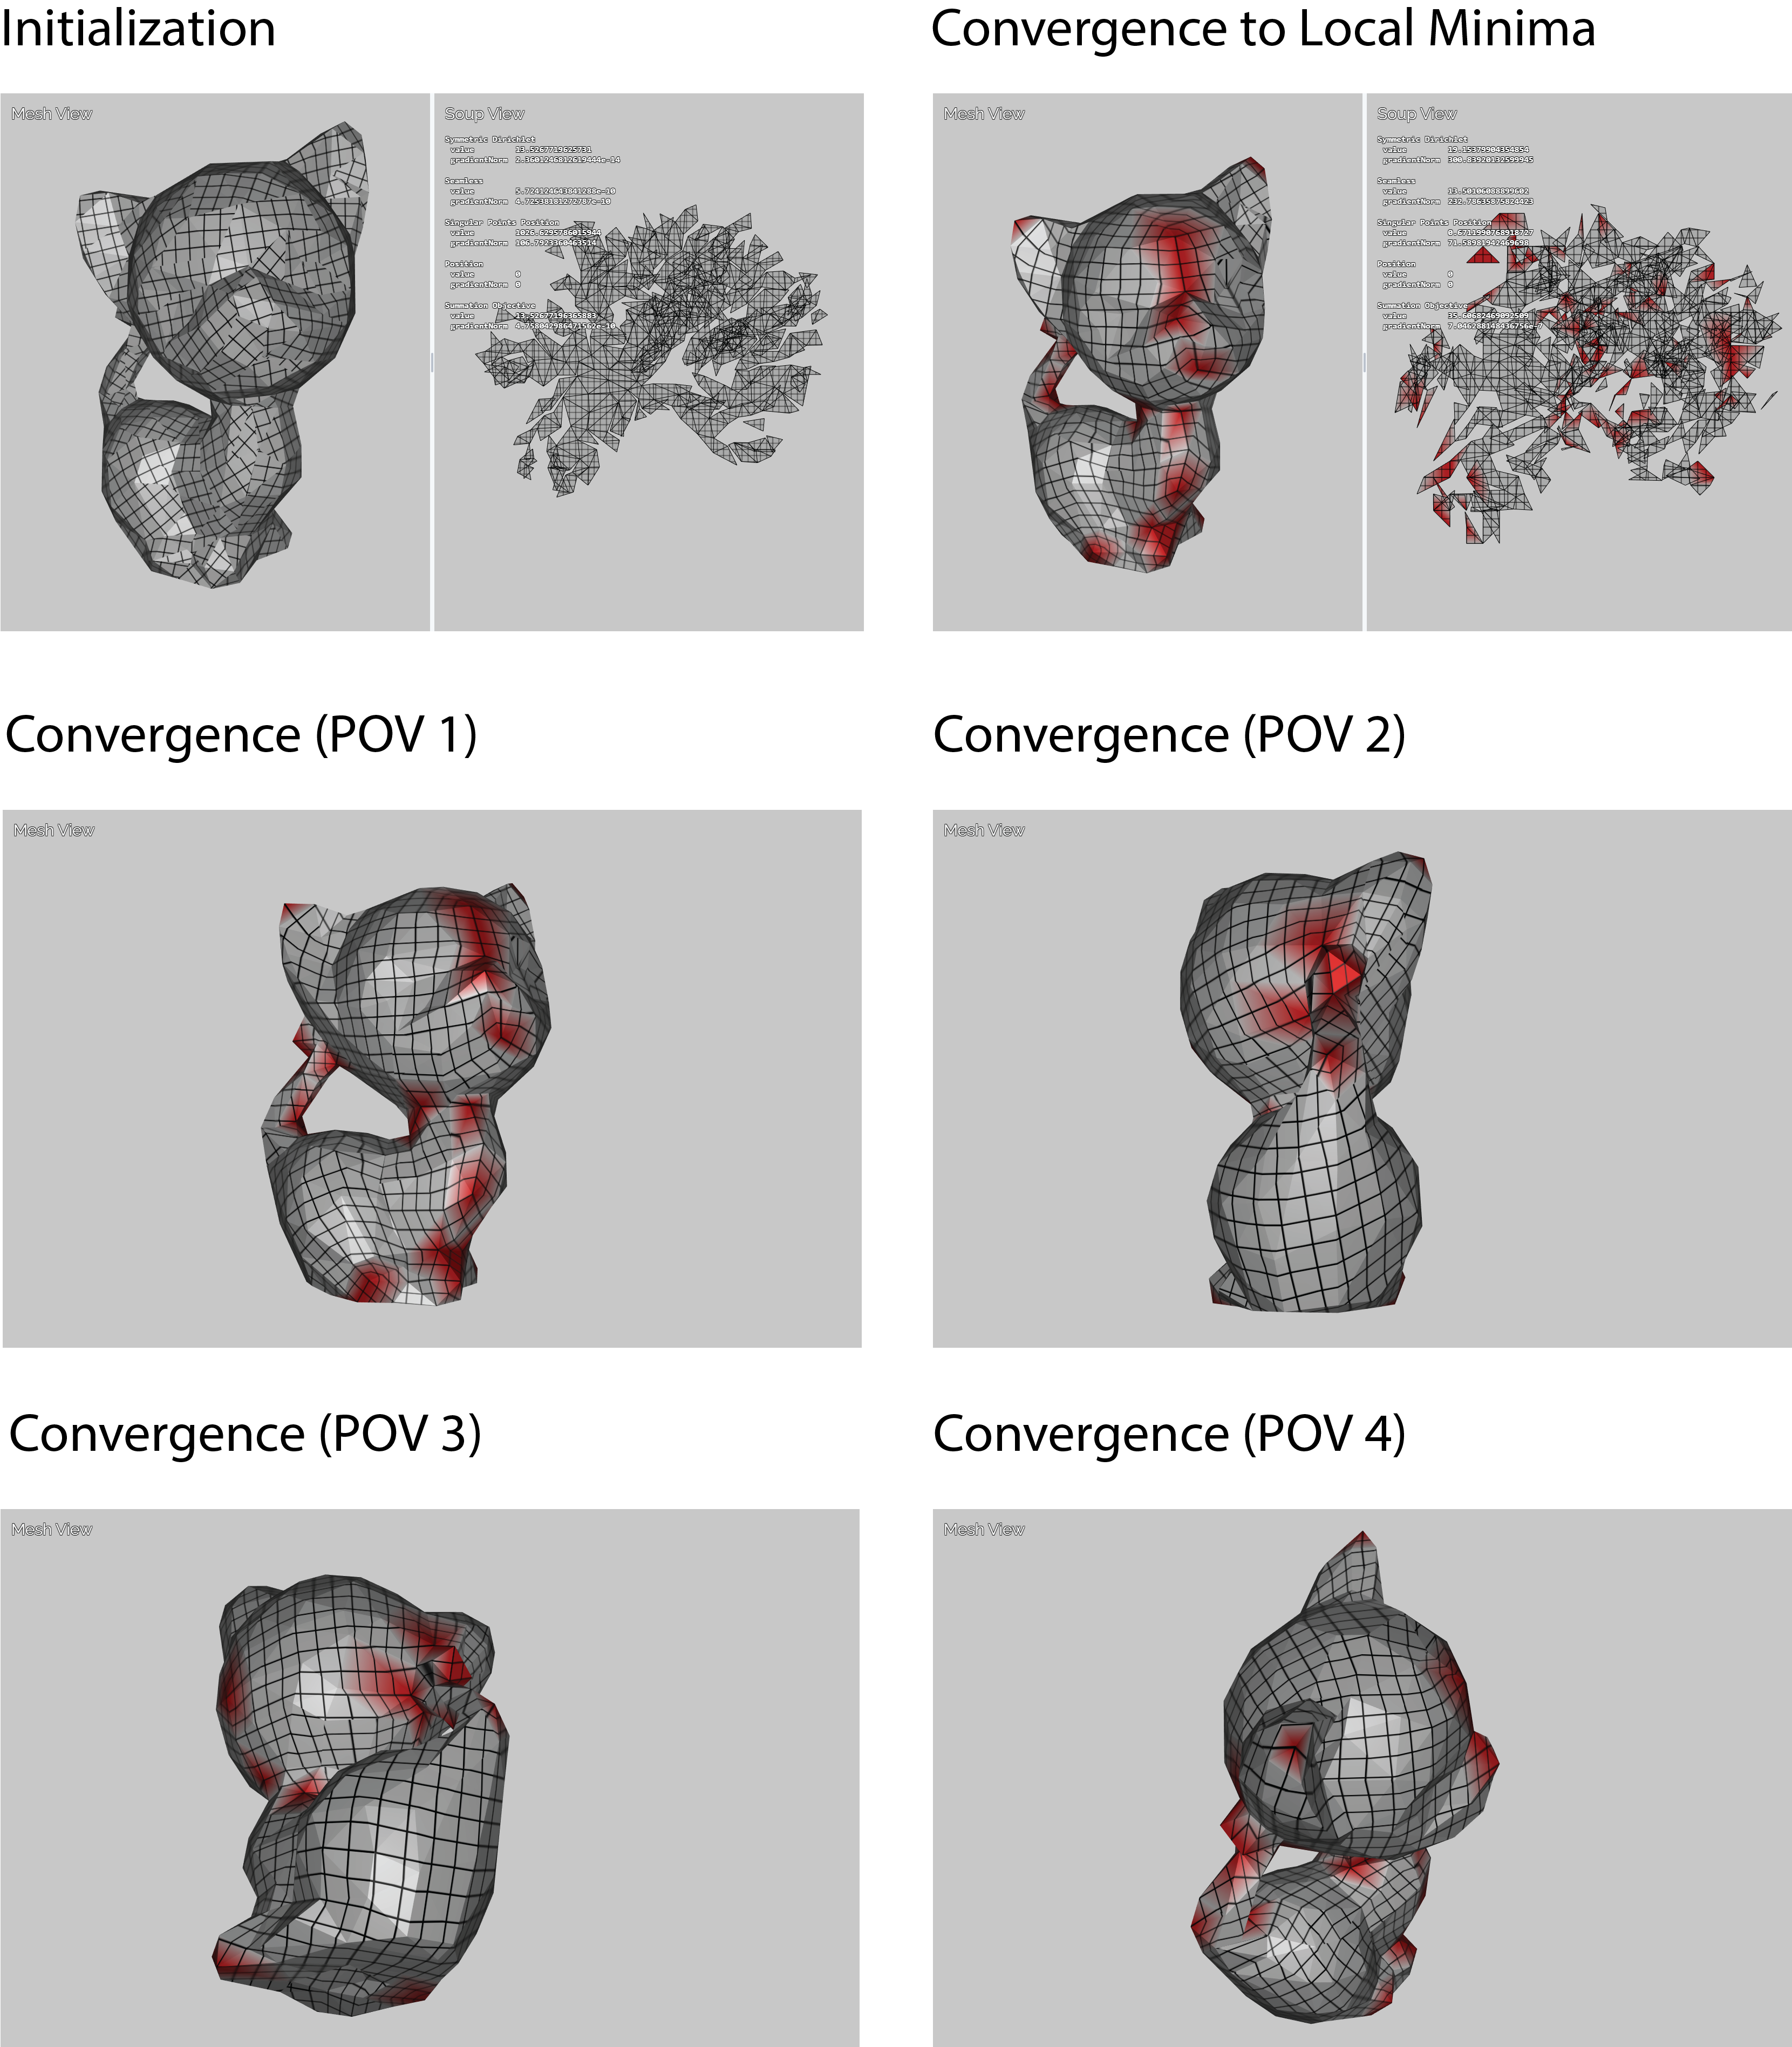
\includegraphics[width=14cm]{figures/results/kitten.png}
\caption[Kitten Model]{}
\end{figure}
\newpage
\section{Octopus Model}
\begin{figure}[ht]
\centering
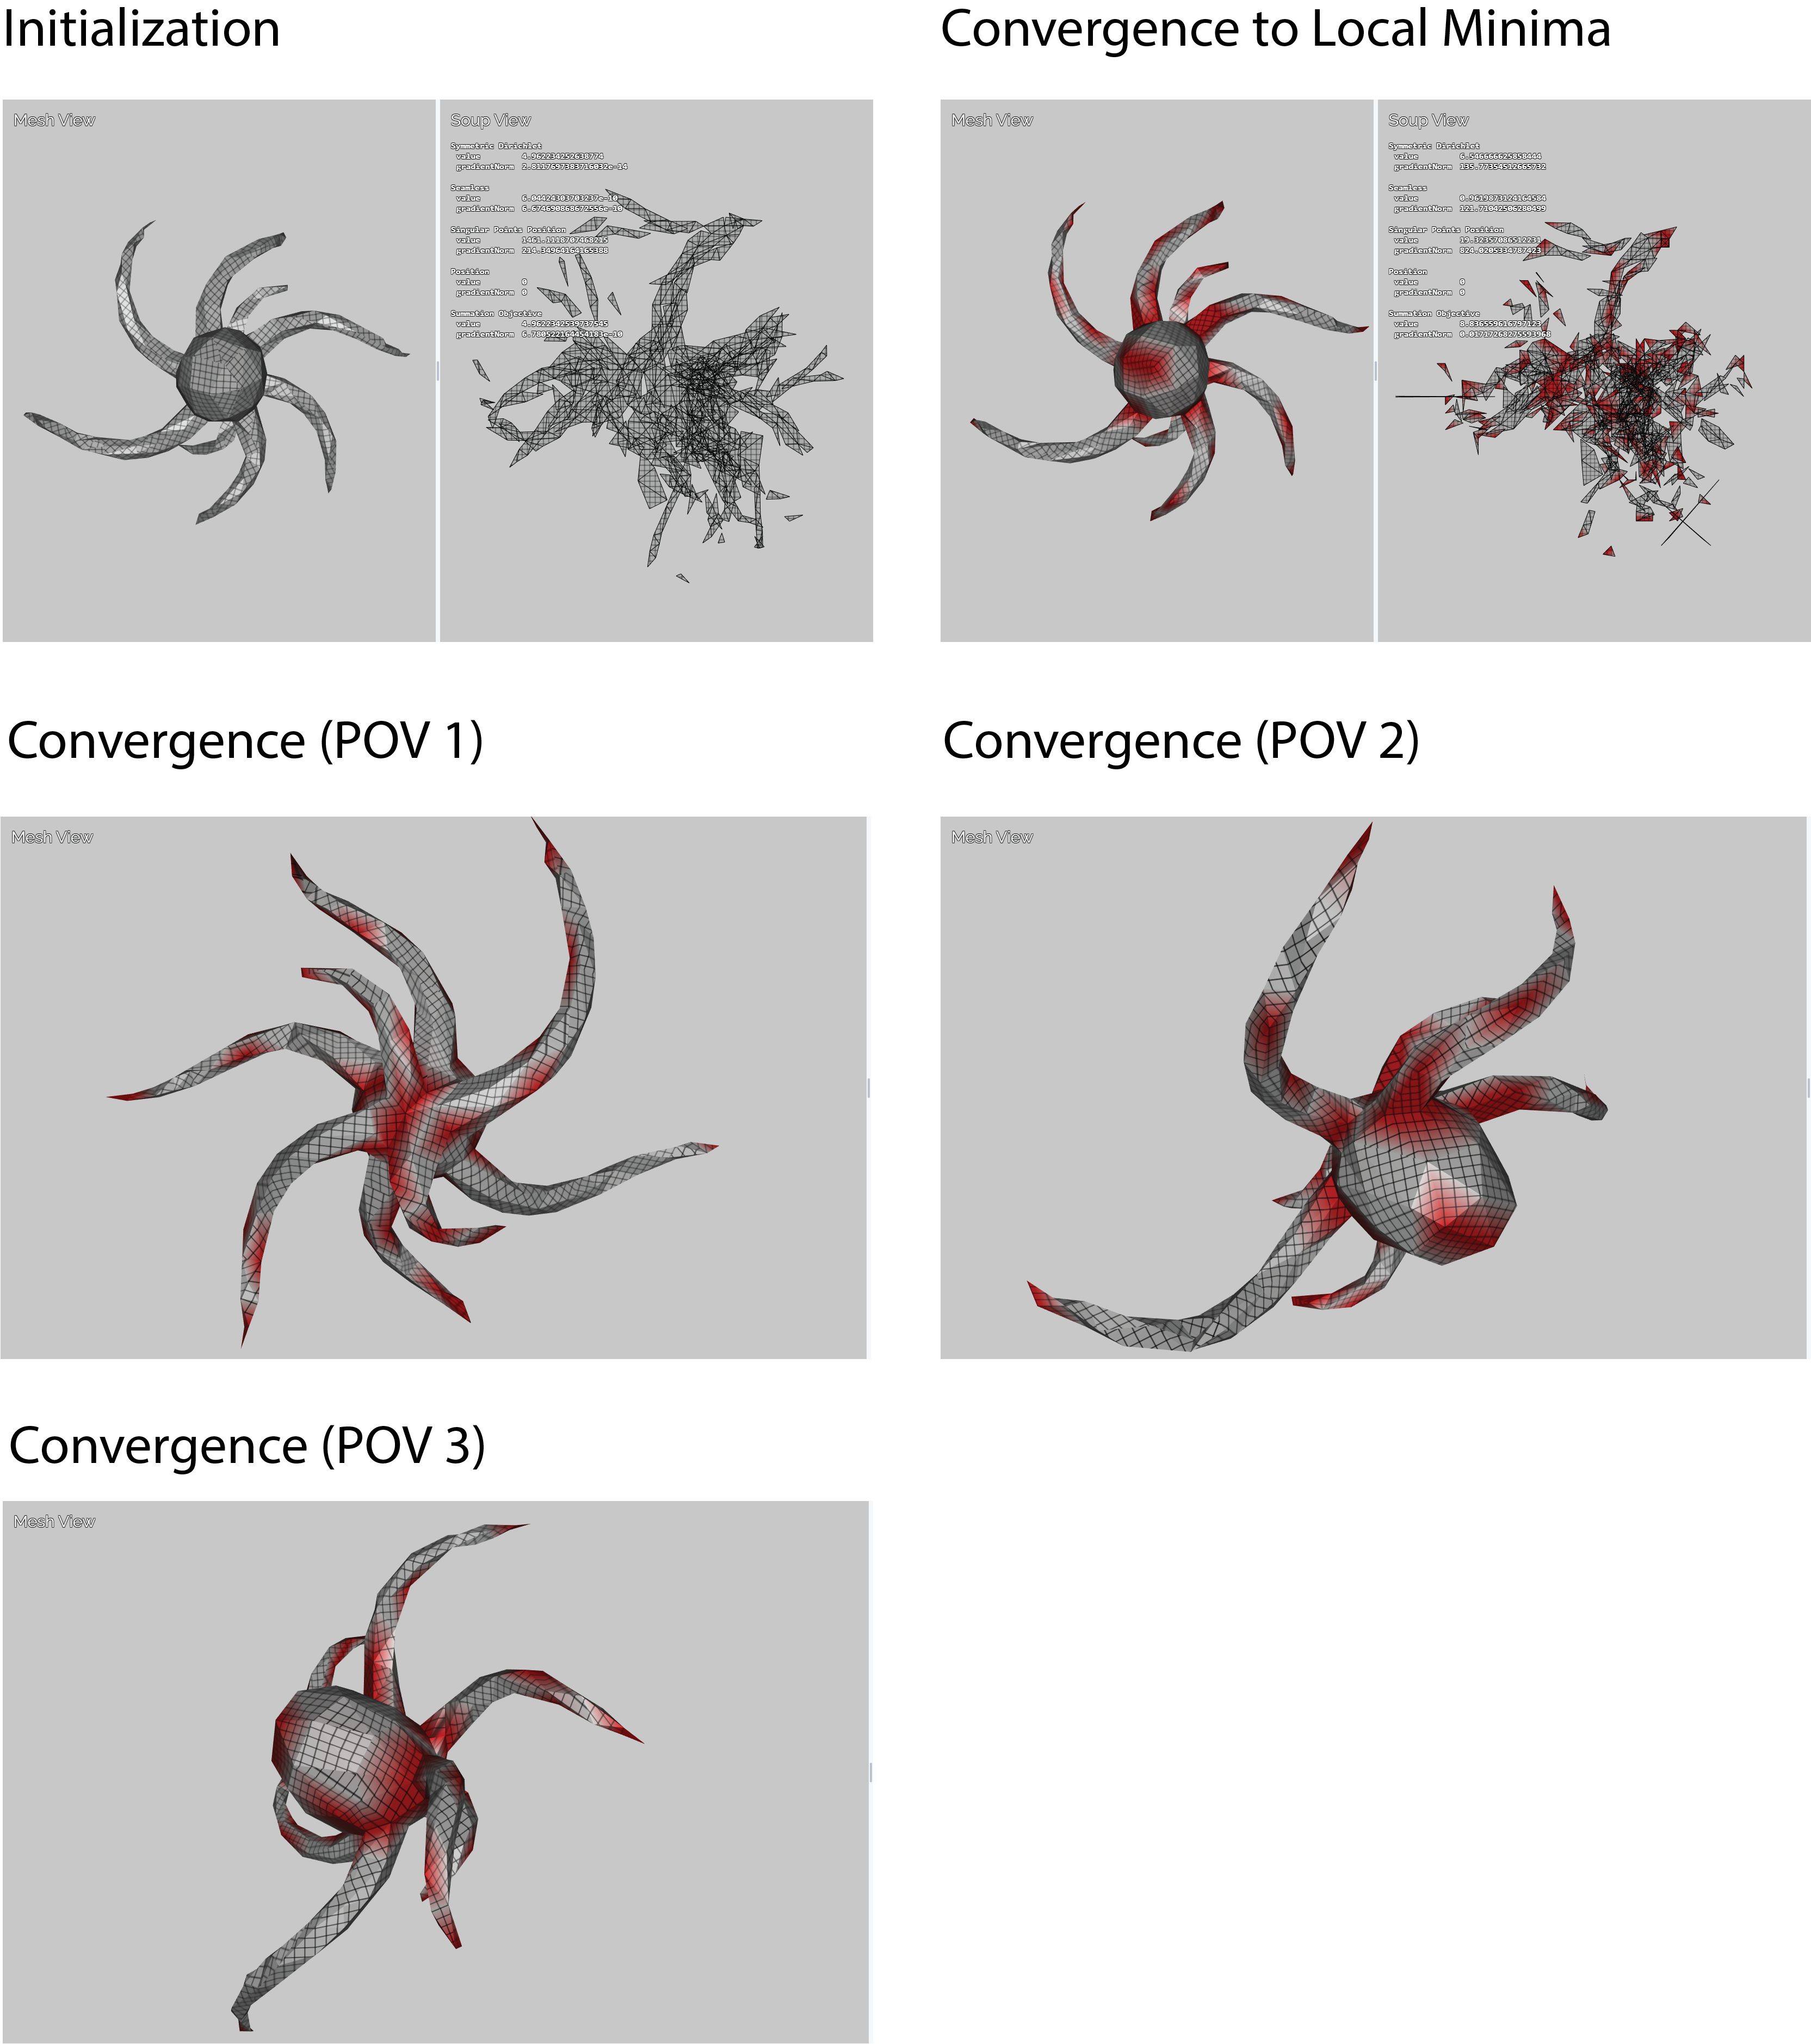
\includegraphics[width=14cm]{figures/results/octopus.png}
\caption[Octopus Model]{}
\end{figure}
\newpage
\section{Venus Model}
\begin{figure}[ht]
\centering
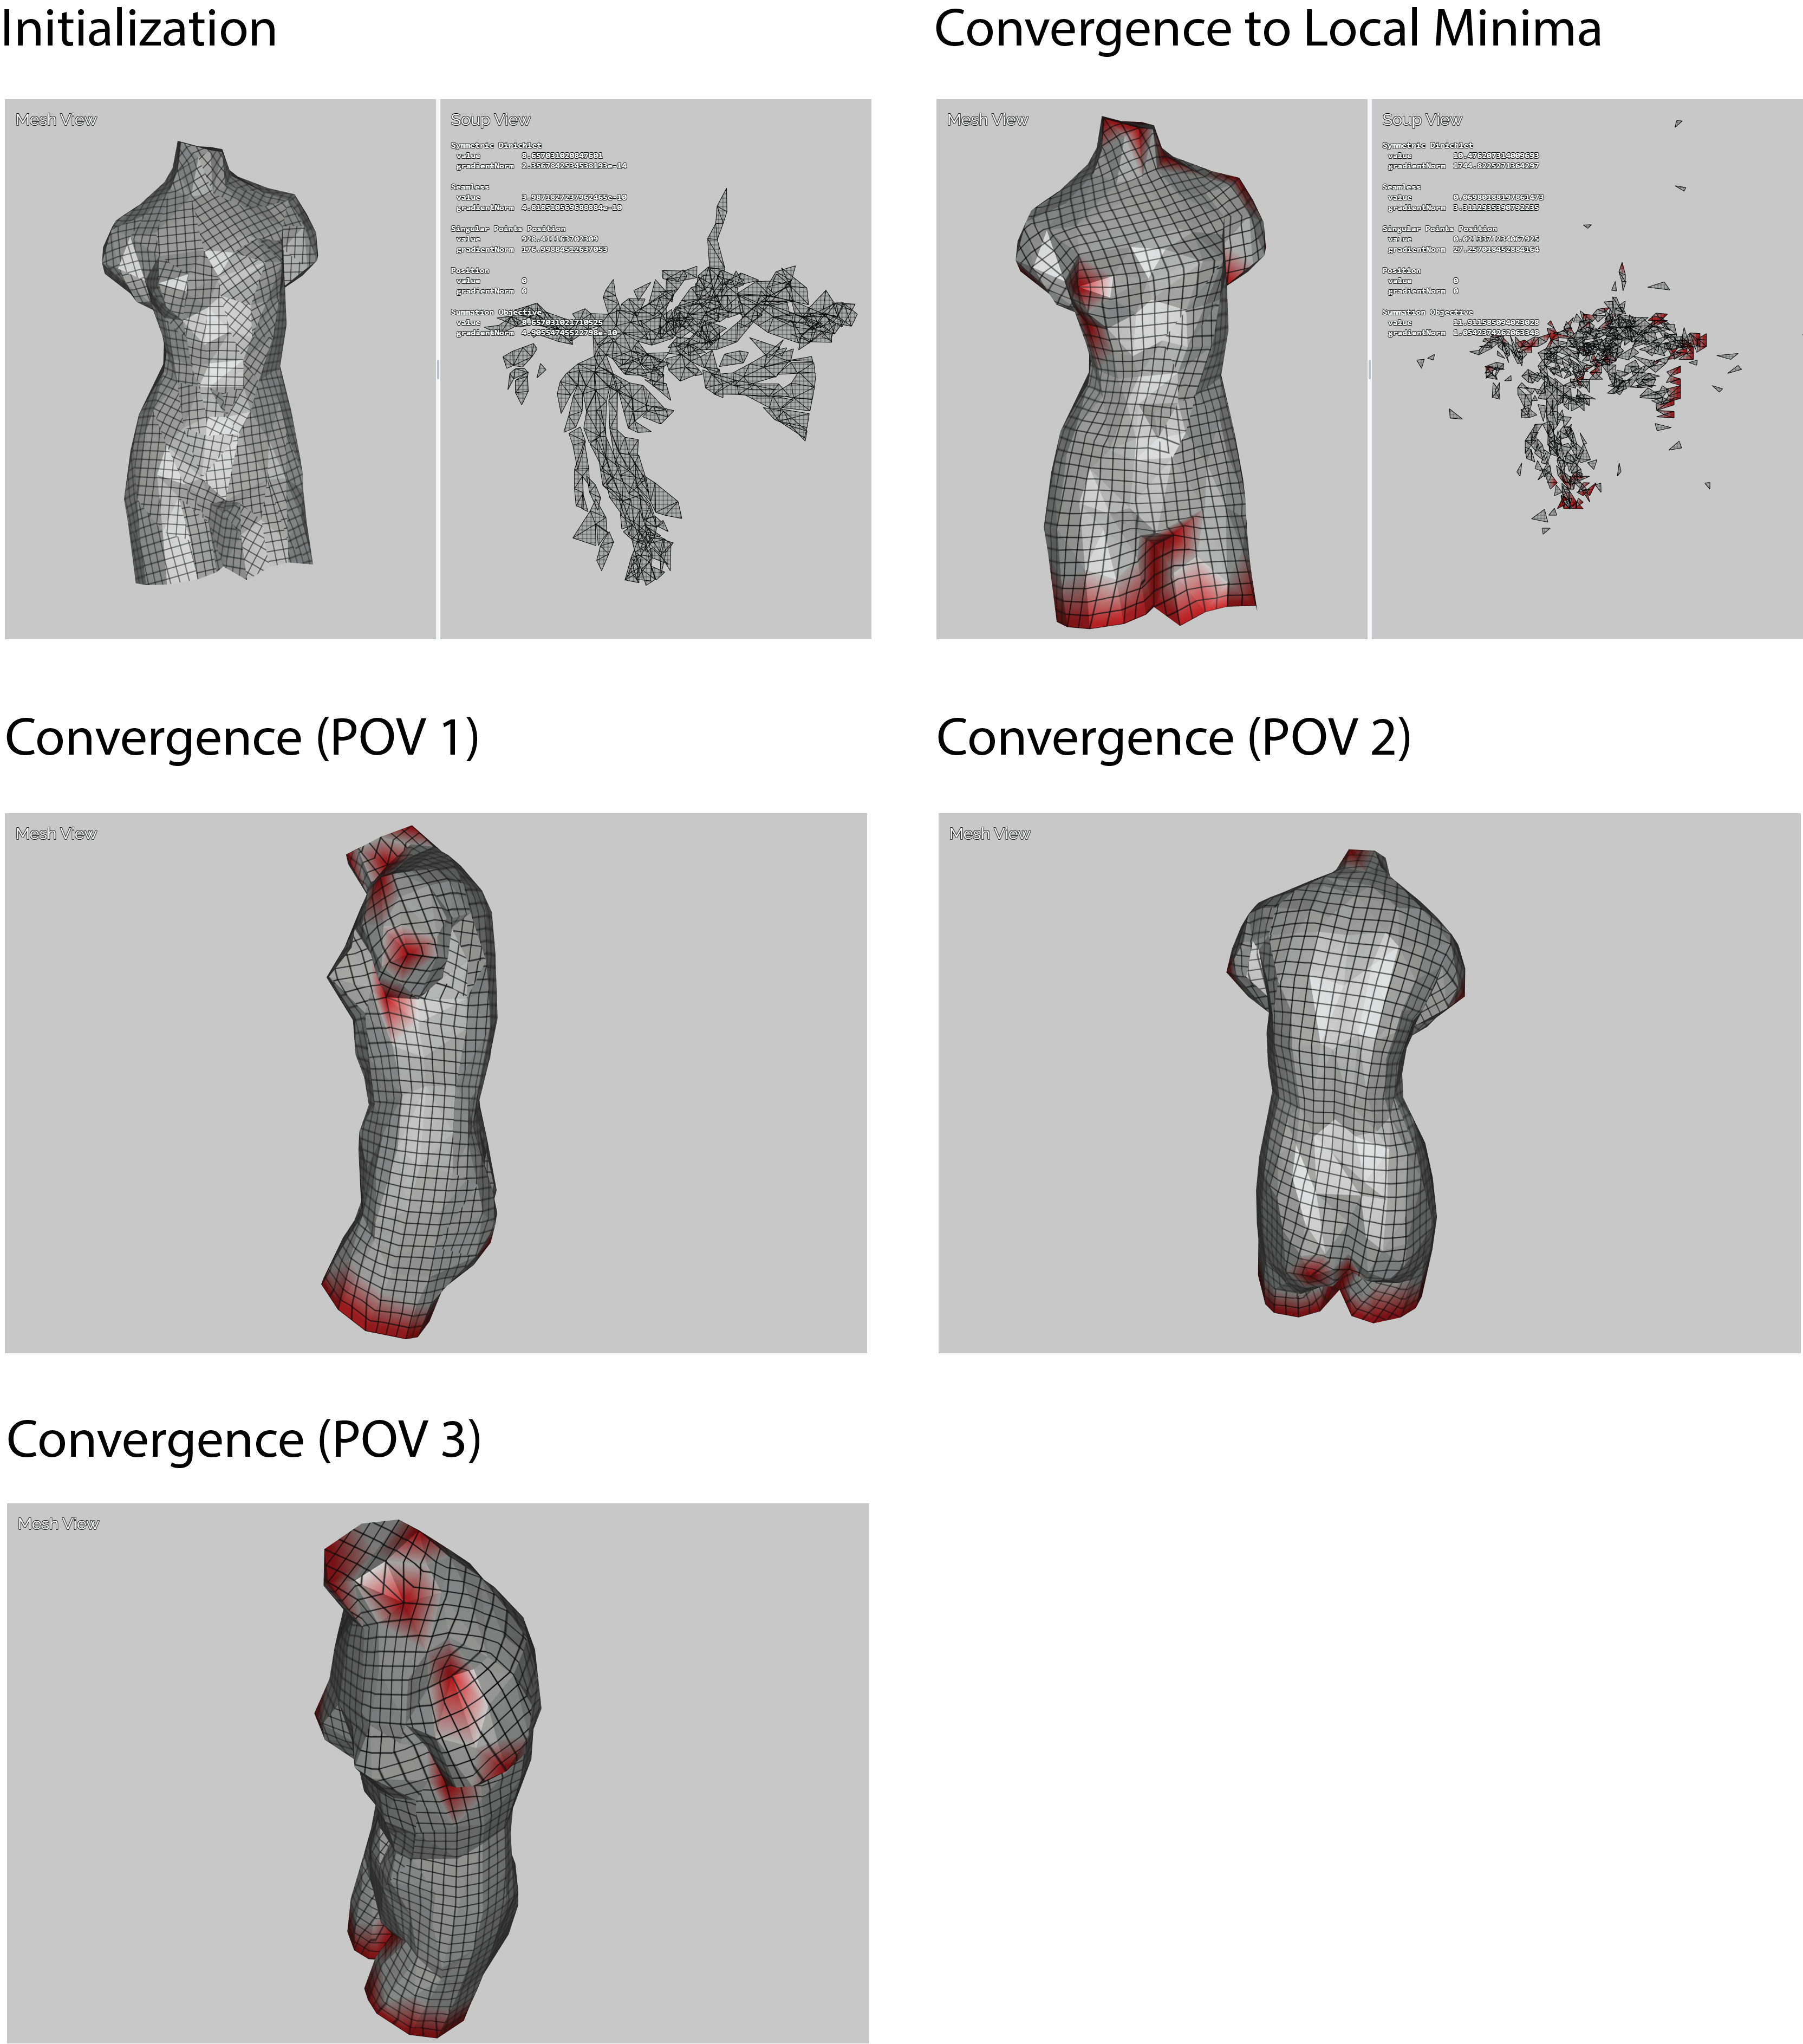
\includegraphics[width=14cm]{figures/results/venus.png}
\caption[Venus Model]{}
\end{figure}
\newpage
\section{Retinal Model}
\begin{figure}[ht]
\centering
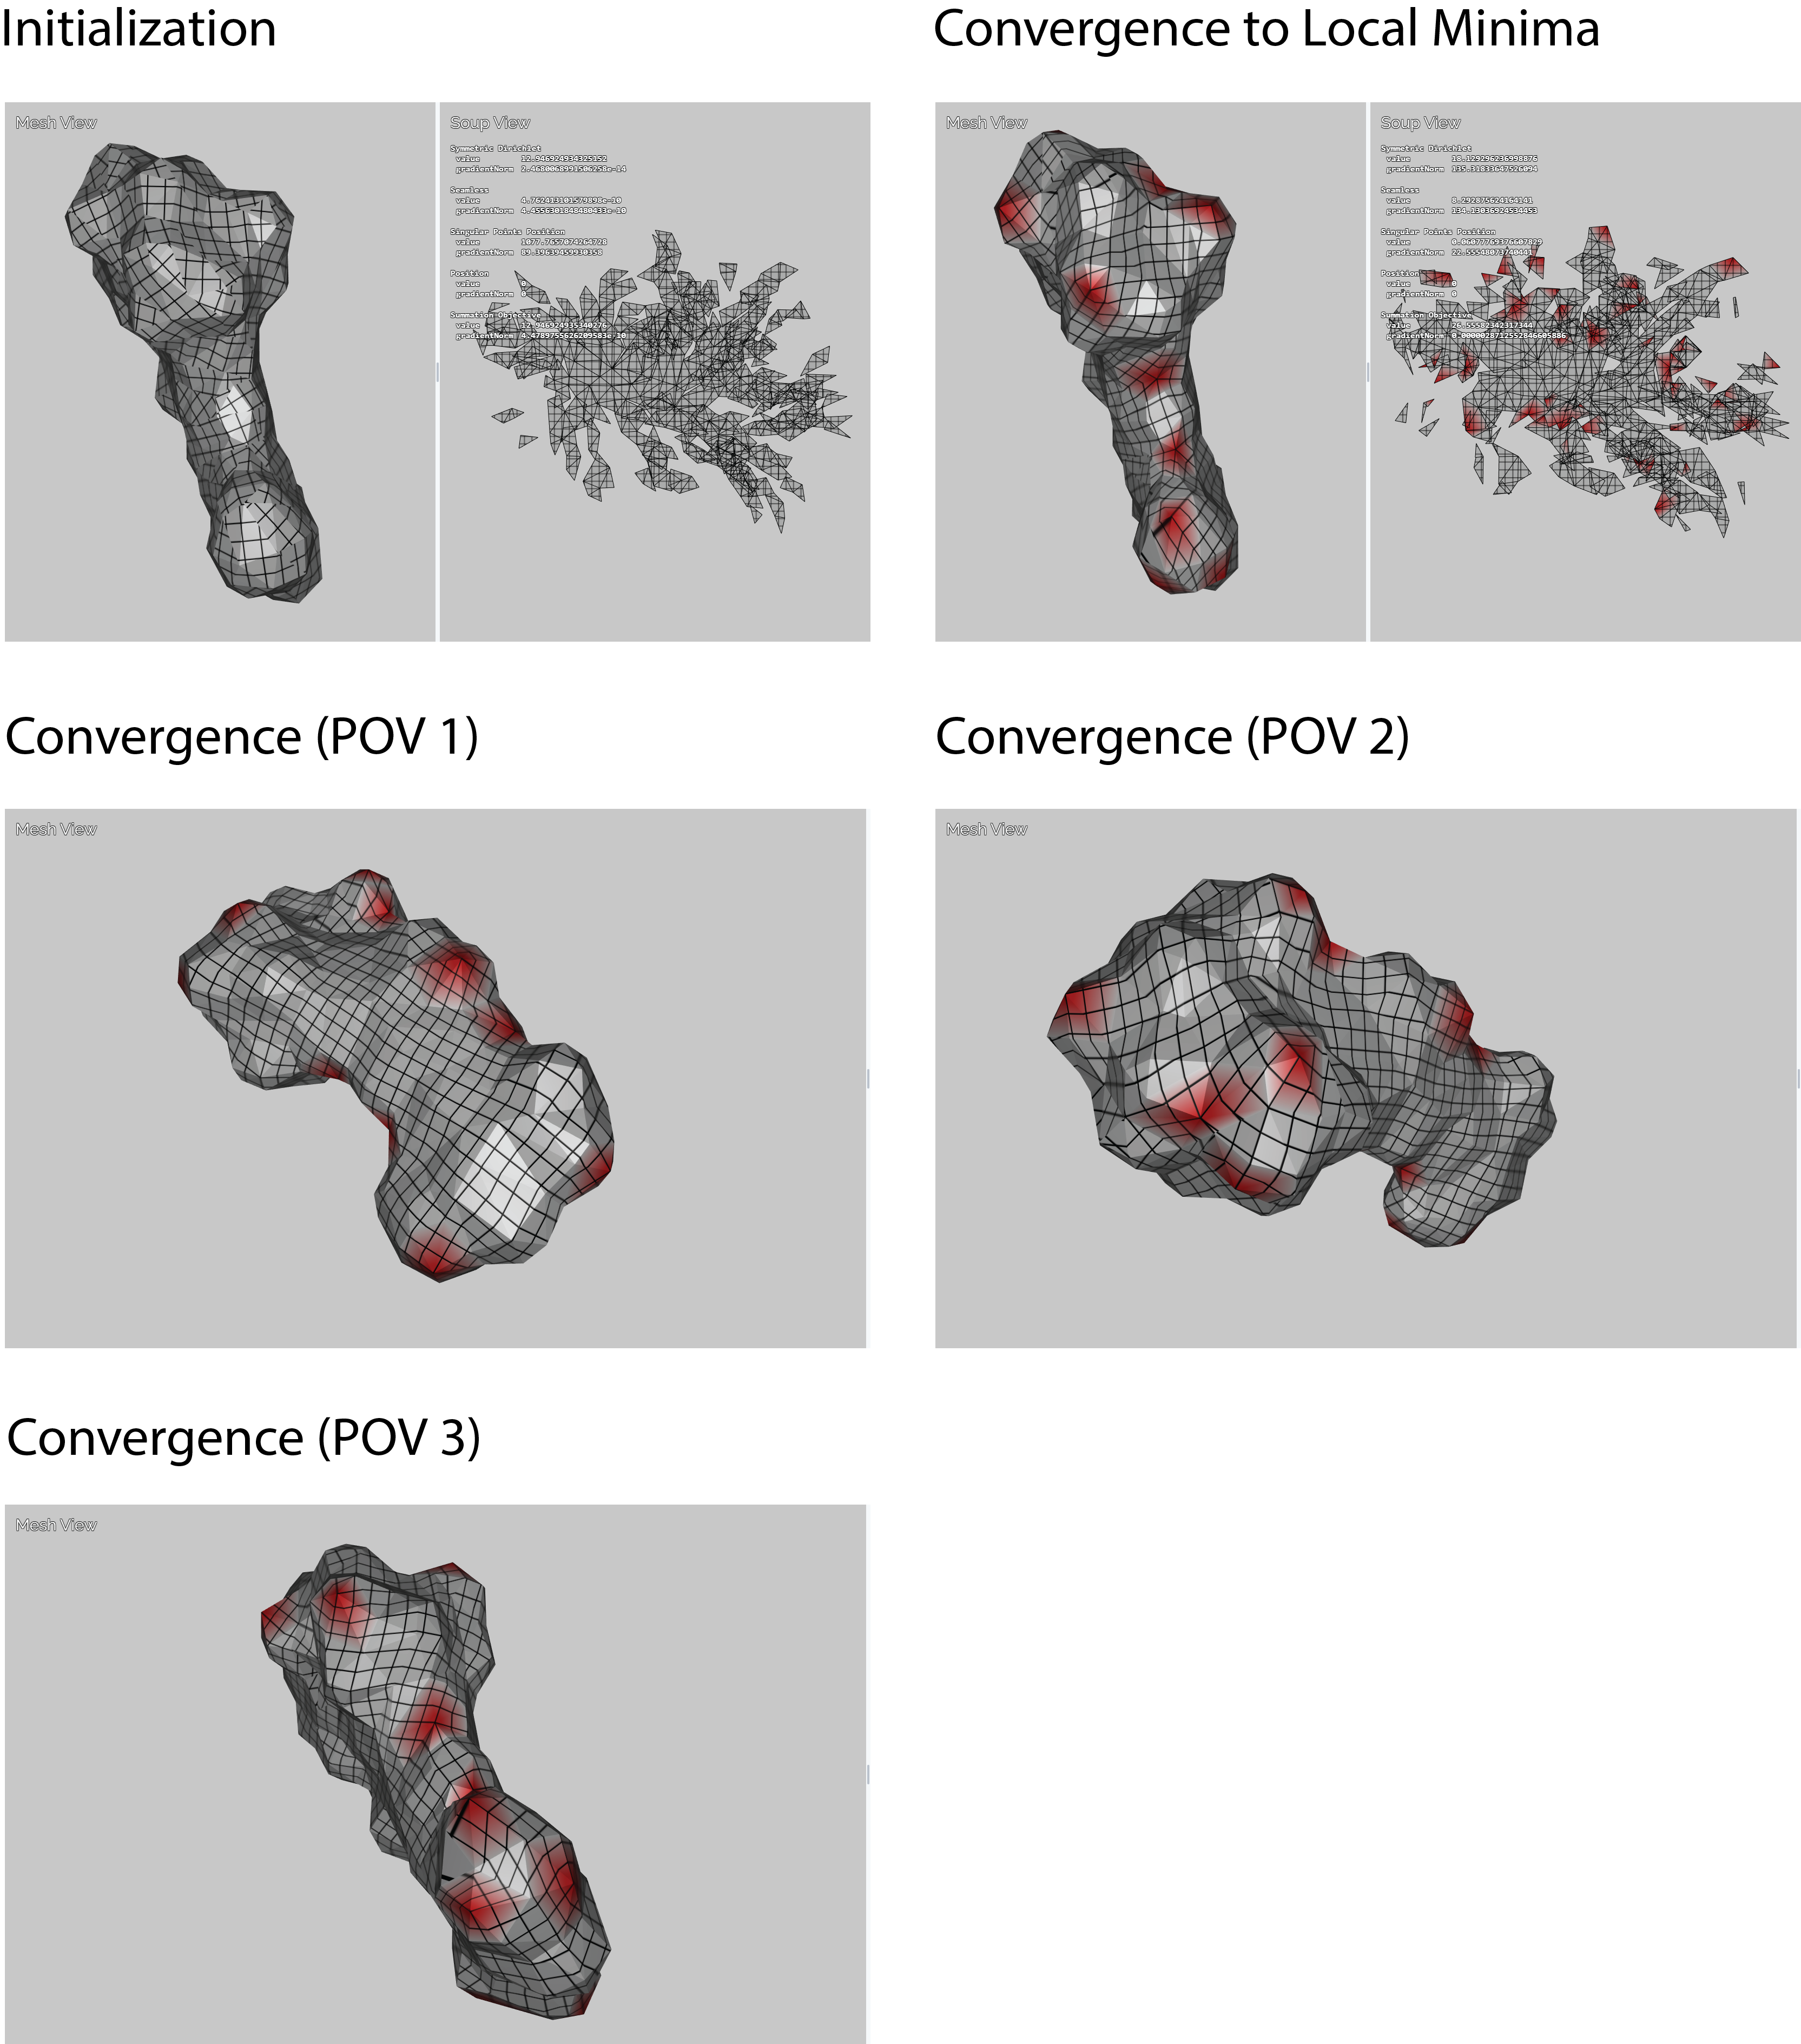
\includegraphics[width=14cm]{figures/results/retinal.png}
\caption[Retinal Model]{}
\end{figure}
\chapter{Concluding Remarks and Future Research}
We have presented a method to quadrangulate a triangle-mesh interactively by solving a smooth unconstrained optimization problem, and designed a tool to demonstrate it in action. Our method produce decent preliminary results, but yet to be sufficient for extracting a quad mesh. As can be seen in chapter \ref{chapter:results}, the Cartesian grid isolines do form a valid quad mesh over the 3D surface of the presented models, but failures can be spotted where the isolines are discontinues. Figure \ref{fig:failues} demonstrate surface areas where our method failed to satisfy the integer-grid maps conditions.
\begin{figure}[ht]
\centering
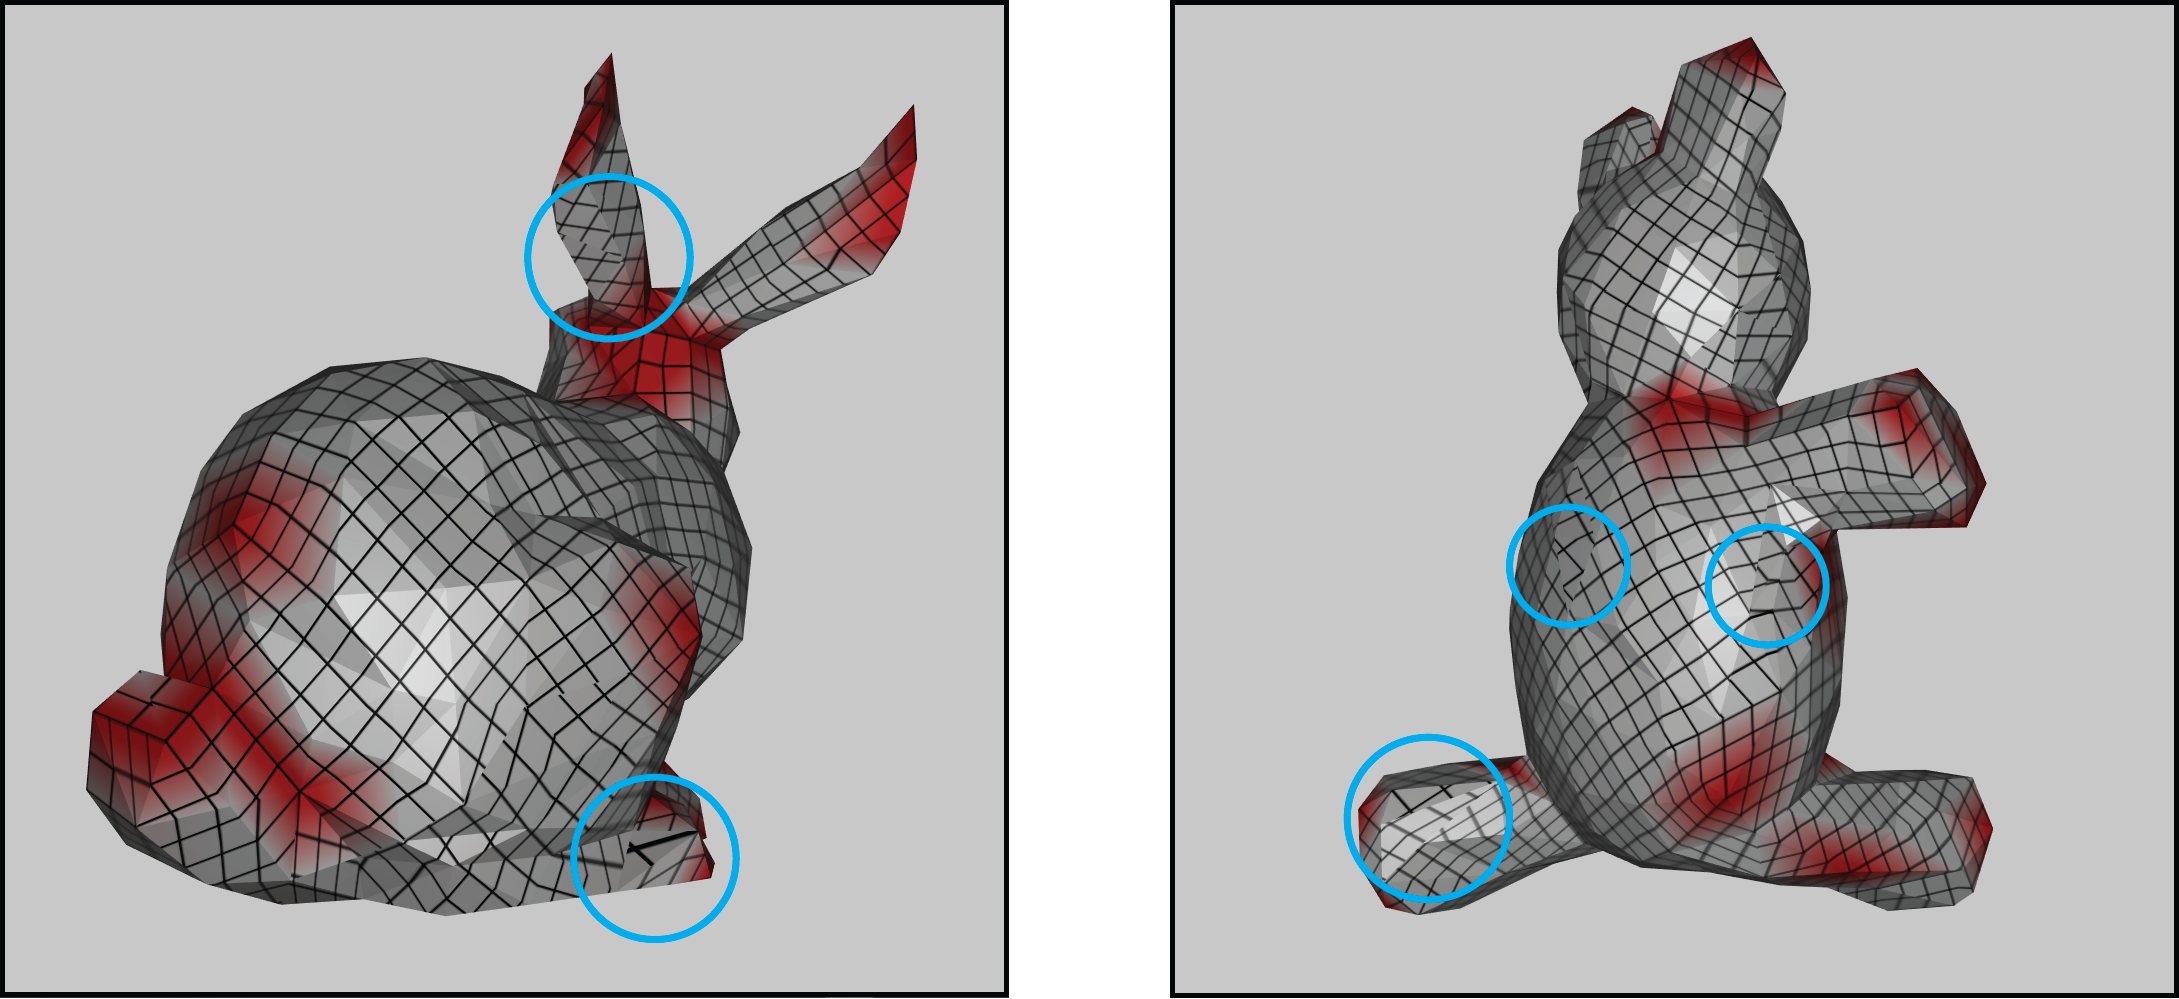
\includegraphics[width=13cm]{figures/results/failures.png}
\caption[Failure Spots of Our Method]{The blue circles mark areas on the surfaces where the continuity of the Cartesian isolines breaks}
\label{fig:failues}
\end{figure}

\noindent We believe our method can be further improved, both by means of its penalty functions formulation and by its graphic user interface. We present numerous ideas for future research work:
\paragraph{Unified Penalty Function for Angle and Length}
The separation between the angle and length penalty functions is technical and artificial, it makes it harder for the end-user to control the optimization process, and it introduce unnecessary inconsistent sensitivity for weight perturbations. We propose to use instead the following penalty function for two half-edges $e_i$ and $e_j$:
\begin{flalign}
P_{unified} = \norm{R\left(e_i, e_j\right)^4 - I}_F^2
\end{flalign}
Where $R\left(e_i, e_j\right)$ is the linear transformation induced by the two coordinate system defined by $e_i$ and $e_j$, when treated as vector sharing the same origin. Figure \ref{fig:unified} the two coordinate systems that defines $R\left(e_i, e_j\right)$. If $R\left(e_i, e_j\right)^4$ equals the identity matrix, then the two half-edges must have the same length be an integer multiple of $90^\circ$ degrees apart.
\begin{figure}[ht]
\centering
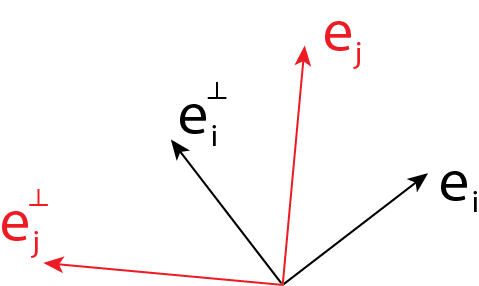
\includegraphics[width=8cm]{figures/unified_energy.png}
\caption[Unified Energy Coordinate Systems]{$R\left(e_i, e_j\right)$ is the linear transformation that takes the black vector onto their corresponding red vectors.}
\label{fig:unified}
\end{figure}
\paragraph{Orientation Field}
We believe that we can achieve superior results by aligning the partial derivative vectors of the parametrization mapping with the principal curvature directions, or any other given orientation field, such as brush strokes painted by the user. To achieve it, one can formulate an additional penalty function, as described in \cite{10.1145/1531326.1531383}.
\paragraph{Manual Location of Singular-Points}
We believe that the user can have a great benefit from being able to manually select where singular-points will be located. To achieve it, it is possible to define an additional penalty function, which will penalize set of twin-vertices for having \textbf{zero} angular defect.
\appendix
\chapter{Polynomial Approximation}
\label{appendix:a}
\section{Piece-wise Polynomial Periodic Function}
To make each Newton's method iteration more computationally efficient, and to simplify the gradient and Hessian derivations and the technical implementation details in general, we design a smooth periodic function $f_p: \mathbb{R} \xrightarrow[]{} \mathbb{R}$ with period $p$, that satisfies the following requirements for any $x \in \mathbb{R}$ and $k \in \mathbb{Z}$:
\begin{equation}\label{eq:periodic_req}
\begin{split}
&0 \leq f_p\left(x\right) \leq 1 \\
&f_p\left(x\right) = f_p\left(x + kp\right) \\
&f_p\left(\frac{p}{2} + kp\right) = 1 \\
&f_p\left(kp\right) = 0 \\
\end{split}
\end{equation}
In other words, we simply want its roots to be periodic. We achieve it by finding a polynomial $g\left(x\right)$ that satisfies requirements \ref{eq:periodic_req} in the interval $\left[0, p\right]$, and replicating it over the whole real-numbers domain. Explicitly, we want the polynomial to satisfy the following:
\begin{equation}\label{eq:system_of_equations}
\begin{split}
&g\left(0\right) = 0, \quad,
g\left(\frac{p}{2}\right) = 1, \quad,
g\left(p\right) = 0 \\ \\
&\frac{dg}{dx}\left(0\right) = 0, \quad
\frac{dg}{dx}\left(\frac{p}{2}\right) = 0, \quad
\frac{dg}{dx}\left(p\right) = 0
\end{split}
\end{equation}
This suggest that $g\left(x\right)$ is a polynomial of degree 6. Therefore, $g\left(x\right)$ is given by:
\begin{equation}\label{eq:polynomial_6}
\begin{split}
g\left(x\right) = a_0 + a_1x + a_2x^2 + a_3x^3 + a_4x^4 + a_5x^5 = a^T \cdot \mathrm{x}\left(x\right)
\end{split}
\end{equation}
Where $a = \left(a_0,a_1,a_2,a_3,a_4,a_5\right)^T$ and $\mathrm{x}\left(x\right) = \left(1,x,x^2,x^3,x^4,x^5\right)^T$.
Solving the linear system of equations \ref{eq:system_of_equations} yields the desired coefficients vector $a_* = \left(a^*_0,a^*_1,a^*_2,a^*_3,a^*_4,a^*_5\right)^T$. Therefore, we define $f_p\left(x\right)$ as follows:
\begin{equation}\label{eq:polynomial_6}
\begin{split}
f_p\left(x\right) = 
\begin{cases} 
  g_*\left(x\right) & x \in \left[0,p\right] \\
  g_*\left(x \mod{p}\right) & x \notin \left[0,p\right]
\end{cases}
\end{split}
\end{equation}
Where $g_*\left(x\right) = a_*^T \cdot \mathrm{x}\left(x\right)$. We call $f_p\left(x\right)$ a \emph{piece-wise polynomial periodic function}. Figure \ref{fig:polynomial_periodic_function} visualize $f_p\left(x\right)$ for an arbitrary period.
\begin{figure}[ht]
\centering
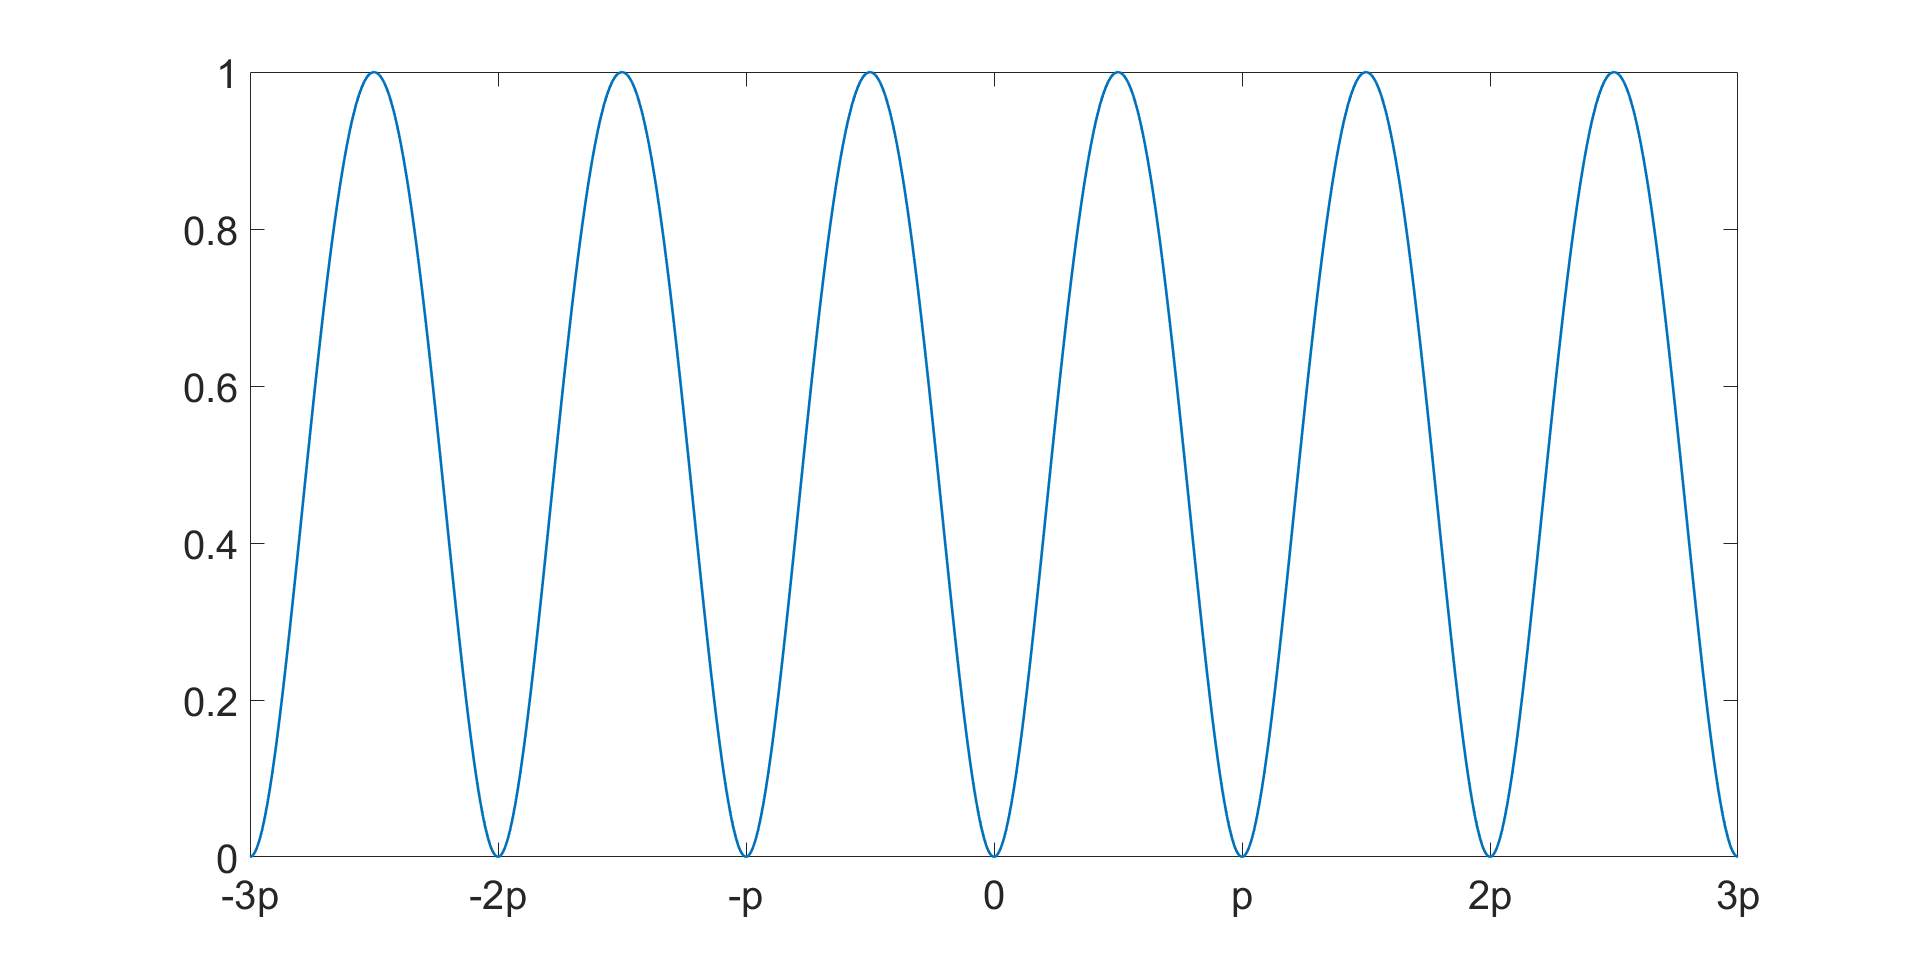
\includegraphics[width=12cm]{figures/periodic_function.png}
\caption[Piece-wise Polynomial Periodic Function]{A plot of $f_p\left(x\right)$ in the interval $\left[-3p, 3p\right]$. As can be seen, $f_p\left(x\right)$ is a priodic function, where its roots are equally spaced with a distance $p$.}
\label{fig:polynomial_periodic_function}
\end{figure}
\section{First Derivative}
The first derivative of $g_*\left(x\right)$ is given by:
\begin{equation}\label{eq:polynomial_6}
\begin{split}
g'_*\left(x\right) = a^*_1 + 2a^*_2x + 3a^*_3x^2 + 4a^*_4x^3 + 5a^*_5x^4 = b_*^T \cdot \mathrm{x}\left(x\right)
\end{split}
\end{equation}
Where $b_* = \left(a^*_1,2a^*_2,3a^*_3,4a^*_4,5a^*_5,0\right)^T$ and $\mathrm{x}\left(x\right) = \left(1,x,x^2,x^3,x^4,x^5\right)^T$. Therefore, we define $f'_p\left(x\right)$ is given as follows:
\begin{equation}\label{eq:polynomial_6}
\begin{split}
f'_p\left(x\right) = 
\begin{cases} 
  g'_*\left(x\right) & x \in \left[0,p\right] \\
  g'_*\left(x \mod{p}\right) & x \notin \left[0,p\right]
\end{cases}
\end{split}
\end{equation}
\section{Second Derivative}
The second derivative of $g_*\left(x\right)$ is given by:
\begin{equation}\label{eq:polynomial_6}
\begin{split}
g''_*\left(x\right) = 2a^*_2 + 6a^*_3x + 12a^*_4x^2 + 20a^*_5x^3 = c_*^T \cdot \mathrm{x}\left(x\right)
\end{split}
\end{equation}
Where $c_* = \left(2a^*_2,6a^*_3, 12a^*_4,20a^*_5,0,0\right)^T$ and $\mathrm{x}\left(x\right) = \left(1,x,x^2,x^3,x^4,x^5\right)^T$. Therefore, we define $f''_p\left(x\right)$ is given as follows:
\begin{equation}\label{eq:polynomial_6}
\begin{split}
f''_p\left(x\right) = 
\begin{cases} 
  g''_*\left(x\right) & x \in \left[0,p\right] \\
  g''_*\left(x \mod{p}\right) & x \notin \left[0,p\right]
\end{cases}
\end{split}
\end{equation}
\chapter{Gradient and Hessian Derivations}
In this appendix, we show detailed derivations for the gradient and Hessian of each individual penalty function, as defined in chapter \ref{chapter:method}.
\section{Composition - General Case}
\label{section:composition_general_case}
Given two smooth functions $f: \mathbb{R}^m \xrightarrow[]{} \mathbb{R}$ and $h: \mathbb{R}^n \xrightarrow[]{} \mathbb{R}^m$, we derive the gradient and Hessian of their composition $g\left(x\right) = f \circ h \left(x\right)$.
\subsection{Gradient}
The differential of  $g\left(x\right)$ is computed as follows:
\begin{flalign}
dg\left(x\right) &= d\bigg(f\Big(h\left(x\right)\Big)\bigg) \\ &= \nabla f\Big(h\left(x\right)\Big)^T \cdot dh\left(x\right)
\\
& = \nabla f \Big(h\left(x\right)\Big)^T \cdot J_h\left(x\right) \cdot dx
\\
& = \bigg(J_h\left(x\right)^T \cdot \nabla f\Big(h\left(x\right)\Big)\bigg)^T \cdot dx \label{eq:generalized_composition_gradient}
\end{flalign}
By \ref{eq:generalized_composition_gradient} we get that the gradient $\nabla g\left(x\right)$ is given by:
\begin{flalign}
\nabla g\left(x\right) = J_h\left(x\right)^T \cdot \nabla f\Big(h\left(x\right)\Big)
\end{flalign}
Where $J_h\left(x\right)$ is the Jacobian matrix of $h$ at $x$.
\subsection{Hessian}
The differential of $\nabla g\left(x\right)$ is computed as follows:
\begin{flalign}
d \nabla g \left(x\right) &= d\bigg( J_h\left(x\right)^T \cdot \nabla f\Big(h\left(x\right)\Big) \bigg)
\\
&= d J_h\left(x\right)^T \cdot \nabla f\Big(h\left(x\right)\Big) + J_h\left(x\right)^T \cdot d \nabla f\Big(h\left(x\right)\Big)
\\
&= \Big(d J_h\left(x\right)\Big)^T \cdot \nabla f\Big(h\left(x\right)\Big) + J_h\left(x\right)^T \cdot d \nabla f\Big(h\left(x\right)\Big)
\\
&= \Big(T_h\left(x\right)dx\Big)^T \cdot \nabla f\Big(h\left(x\right)\Big) + J_h\left(x\right)^T \cdot \nabla^2 f\Big(h\left(x\right)\Big) \cdot dh\left(x\right)
\\
&= dx^T \cdot T_h\left(x\right)^T \cdot \nabla f\Big(h\left(x\right)\Big) + J_h\left(x\right)^T \cdot \nabla^2 f\Big(h\left(x\right)\Big) \cdot J_h\left(x\right) \cdot dx
\\
&= \bigg(T_h\left(x\right)^T \cdot \nabla f\Big(h\left(x\right)\Big)\bigg)^T \cdot dx + J_h\left(x\right)^T \cdot \nabla^2 f\Big(h\left(x\right)\Big) \cdot J_h\left(x\right) \cdot dx
\\
&= \underbrace{\nabla f\Big(h\left(x\right)\Big)^T \cdot T_h\left(x\right)}_{\text{$n \times n$ matrix}} \cdot dx + \underbrace{J_h\left(x\right)^T \cdot \nabla^2 f\Big(h\left(x\right)\Big) \cdot J_h\left(x\right)}_{\text{$n \times n$ matrix}} \cdot dx
\\
&= \bigg( \nabla f\Big(h\left(x\right)\Big)^T \cdot T_h\left(x\right) + J_h\left(x\right)^T \cdot \nabla^2 f\Big(h\left(x\right)\Big) \cdot J_h\left(x\right) \bigg) \cdot dx
\label{eq:generalized_composition_hessian}
\end{flalign}
By \ref{eq:generalized_composition_hessian} we get that the Hessian $\nabla^2 g\left(x\right)$ is given by:
\begin{flalign}
\nabla^2 g \left(x\right) = \nabla f\Big(h\left(x\right)\Big)^T \cdot T_h\left(x\right) + J_h\left(x\right)^T \cdot \nabla^2 f\Big(h\left(x\right)\Big) \cdot J_h\left(x\right)
\end{flalign}
Where $T_h\left(x\right)$ is a tensor of $n$ matrices, each of size $m \times n$.
\subsection{Derivation of $T_h\left(x\right)$}
Let the components of $h\left(x\right)$ be defined as follows:
\begin{flalign}
    h\left(x\right) &= \begin{bmatrix}
           h_1\left(x\right) \\
           \vdots \\
           h_m\left(x\right)
         \end{bmatrix}
\end{flalign}
Such that $h_i\left(x\right): \mathbb{R}^n \xrightarrow[]{} \mathbb{R}$ for $i \in \left\{1,2,\hdots,m\right\}$. Using that explicit definition of $h\left(x\right)$, we get that the Jacobian $J_h\left(x\right)$ is given by:
\begin{flalign}
    J_h\left(x\right) &= \begin{bmatrix}
           \nabla h_1\left(x\right)^T \\
           \vdots \\
           \nabla h_m\left(x\right)^T
         \end{bmatrix}
\end{flalign}
The differential of $J_h\left(x\right)$ is given as follows:
\begin{flalign}
    dJ_h\left(x\right) &= \begin{bmatrix}
           d\nabla h_1\left(x\right)^T \\
           \vdots \\
           d\nabla h_m\left(x\right)^T
         \end{bmatrix}
\\
    &= \begin{bmatrix}
               \Big(d\nabla h_1\left(x\right)\Big)^T \\
               \vdots \\
               \Big(d\nabla h_m\left(x\right)\Big)^T
             \end{bmatrix}
\\
    &= \begin{bmatrix}
               \Big(\nabla^2 h_1\left(x\right) \cdot dx\Big)^T \\
               \vdots \\
               \Big(\nabla^2 h_m\left(x\right) \cdot dx\Big)^T
             \end{bmatrix}
\end{flalign}
Let $\mathrm{row}_i\Big(\nabla^2 h_j\left(x\right)\Big)$ be a function that returns the $i$th row of a given matrix. Let $M_i\left(x\right)$ be a matrix of size $m \times n$ defined as follows:
\begin{flalign}
    M_i\left(x\right) &=
    \begin{bmatrix}
       \mathrm{row}_i\Big(\nabla^2 h_1\left(x\right)\Big) \\
       \vdots \\
       \mathrm{row}_i\Big(\nabla^2 h_m\left(x\right)\Big) \\
    \end{bmatrix}
\end{flalign}
We now can rewrite $dJ_h\left(x\right)$ as follows:
\begin{flalign}
    dJ_h\left(x\right) &=
    \begin{bmatrix}
       M_1\left(x\right) dx & \hdots & M_n\left(x\right) dx
    \end{bmatrix}
    \\
    &= 
    \begin{bmatrix}
       M_1\left(x\right) & \hdots & M_n\left(x\right)
    \end{bmatrix} dx \\
    &= 
    T_h\left(x\right) dx
\end{flalign}
Where $T_h\left(x\right) = \begin{bmatrix} M_1\left(x\right) & \hdots & M_n\left(x\right) \end{bmatrix}$.
\section{Composition - Degenerate Case}
Even though the following derivation is a private case of \ref{section:composition_general_case}, we include it as well for clarity. Given two smooth functions $f: \mathbb{R} \xrightarrow[]{} \mathbb{R}$ and $h: \mathbb{R}^n \xrightarrow[]{} \mathbb{R}$, we derive the gradient and Hessian of their composition $f \circ h\left(x\right)$.
\subsection{Gradient}
The differential of  $f\Big(h\left(x\right)\Big)$ is computed as follows:
\begin{flalign}
df\Big(h\left(x\right)\Big) &= f'\Big(h\left(x\right)\Big) \cdot dh\left(x\right)
\\
& = f'\Big(h\left(x\right)\Big) \cdot \nabla h\left(x\right)^T \cdot dx
\\
& = \bigg(f'\Big(h\left(x\right)\Big) \cdot \nabla h\left(x\right)\bigg)^T \cdot dx \label{eq:composition_gradient}
\end{flalign}
By \ref{eq:composition_gradient} we get that the gradient $\nabla f\Big(h\left(x\right)\Big)$ is given by:
\begin{flalign}
\nabla f\Big(h\left(x\right)\Big) = f'\Big(h\left(x\right)\Big) \cdot \nabla h\left(x\right)
\end{flalign}
\subsection{Hessian}
The differential of  $\nabla f\Big(h\left(x\right)\Big)$ is computed as follows:
\begin{flalign}
d \nabla f\Big(h\left(x\right)\Big) &= d\bigg( f'\Big(h\left(x\right)\Big) \cdot \nabla h\left(x\right)\bigg)
\\
& = df'\Big(h\left(x\right)\Big) \cdot \nabla h\left(x\right) + f'\Big(h\left(x\right)\Big) \cdot d\nabla h\left(x\right)
\\
& = f''\Big(h\left(x\right)\Big) \cdot dh\left(x\right) \cdot \nabla h\left(x\right) + f'\Big(h\left(x\right)\Big) \cdot \nabla^2 h\left(x\right) \cdot dx
\\
& = f''\Big(h\left(x\right)\Big) \cdot \underbrace{\nabla h\left(x\right)^T \cdot dx}_{\text{scalar}} \cdot \nabla h\left(x\right) + f'\Big(h\left(x\right)\Big) \cdot \nabla^2 h\left(x\right) \cdot dx
\\
& = f''\Big(h\left(x\right)\Big) \cdot \underbrace{\nabla h\left(x\right) \cdot \nabla h\left(x\right)^T}_{\text{matrix}} \cdot dx + f'\Big(h\left(x\right)\Big) \cdot \nabla^2 h\left(x\right) \cdot dx
\\
& = \bigg(f''\Big(h\left(x\right)\Big) \cdot \nabla h\left(x\right) \cdot \nabla h\left(x\right)^T + f'\Big(h\left(x\right)\Big) \cdot \nabla^2 h\left(x\right)\bigg) \cdot dx
\label{eq:composition_hessian}
\end{flalign}
By \ref{eq:composition_hessian} we get that the Hessian $\nabla^2 f\Big(h\left(x\right)\Big)$ is given by:
\begin{flalign}
\nabla^2 f\Big(h\left(x\right)\Big) = f''\Big(h\left(x\right)\Big) \cdot \nabla h\left(x\right) \cdot \nabla h\left(x\right)^T + f'\Big(h\left(x\right)\Big) \cdot \nabla^2 h\left(x\right)
\end{flalign}








\section{Squared Norm}
In this section, we derive the gradient and Hessian of the squared Euclidean norm $\norm{\cdot}_2^2: \mathbb{R}^n \xrightarrow[]{} \mathbb{R}$.
\subsection{Gradient}
The differential of $\norm{\cdot}_2^2$ is computed as follows:
\begin{flalign}
d\norm{x}_2^2 &= d\left(x^Tx\right) \\
&= \left(dx\right)^Tx + x^Tdx \\
&= x^Tdx + x^Tdx \\
&= 2x^Tdx \\
\label{eq:squared_norm_gradient}
&= \left(2x\right)^Tdx
\end{flalign}
By \ref{eq:squared_norm_gradient} we get that the gradient $\nabla \norm{x}_2^2$ is given by:
\begin{flalign}
\nabla \norm{x}_2^2 = 2x
\end{flalign}
\subsection{Hessian}
The differential of $\nabla \norm{\cdot}_2^2$ is computed as follows:
\begin{flalign}
d\norm{x}_2^2 &= d\left(x^Tx\right) \\
&= \left(dx\right)^Tx + x^Tdx \\
&= x^Tdx + x^Tdx \\
&= 2x^Tdx \\
\label{eq:squared_norm_gradient}
&= \left(2x\right)^Tdx
\end{flalign}
By \ref{eq:squared_norm_gradient} we get that the gradient $\nabla \norm{x}_2^2$ is given by:
\begin{flalign}
\nabla \norm{x}_2^2 = 2x
\end{flalign}




\section{Angle Penalty Function}
The angle penalty functions is given by:
\begin{equation}\label{eq:angle_penalty}
\begin{split}
P_{\mathrm{angle}}\left(e_i,e_j\right) = \mathrm{sin} \bigg( 4\Big(\theta\left(e_i\right) - \theta\left(e_j\right)\Big) - \frac{\pi}{2}\bigg) + 1
\end{split}
\end{equation}
Where $\theta\left(e_k\right) = \mathrm{atan2}\Big(\mathrm{y}\left(v_k^2\right) - \mathrm{y}\left(v_k^1\right), \mathrm{x}\left(v_k^2\right) - \mathrm{x}\left(v_k^1\right)\Big)$ is the angle formed by half-edge $e_k = \left(v^1_k, v^2_k\right)$ with the positive \emph{x-axis} direction, when treated as a vector based at $v_k^1$ and heading $v_k^2$, for $k \in \left\{i,j\right\}$.

\noindent By denoting:
\begin{equation}\label{eq:angle_penalty}
u = \Big(\mathrm{y}\left(v_i^2\right), \mathrm{y}\left(v_i^1\right), \mathrm{x}\left(v_i^2\right), \mathrm{x}\left(v_i^1\right), \mathrm{y}\left(v_j^2\right), \mathrm{y}\left(v_j^1\right), \mathrm{x}\left(v_j^2\right), \mathrm{x}\left(v_j^1\right)\Big)^T
\end{equation}
And by replacing the sine expression with a piece-wise polynomial periodic function $f_p$ with period $p=\frac{\pi}{2}$ (as defined in appendix \ref{appendix:a}), we can rewrite $P_{\mathrm{angle}}$ as follows:
\begin{equation}\label{eq:angle_penalty_rephrased}
\begin{split}
P_{\mathrm{angle}}\left(u\right) = f_{\frac{\pi}{2}} \bigg(h\left(u\right)\bigg)
\end{split}
\end{equation}
Where $h\left(u\right) = \alpha\left(u\right) - \beta\left(u\right)$, and $\alpha$ and $\beta$ are given by $\alpha\left(u\right) = \mathrm{atan2}\Big(u_0 - u_1, u_2 - u_3\Big)$ and $\beta\left(u\right) = \mathrm{atan2}\Big(u_4 - u_5, u_6 -u_7\Big)$.
\noindent Since we already know how to calculate the gradient and Hessian for a composition of smooth functions, we only need to find expressions for $\nabla h\left(u\right)$ and $\nabla^2 h\left(u\right)$.
\subsection{Gradient}
The differential of $h\left(u\right)$ is given by:
\begin{flalign}
dh\left(u\right) &= d\Big(\alpha\left(u\right) - \beta\left(u\right)\Big)
\\
&= \nabla\alpha\left(u\right)^T du - \nabla\beta\left(u\right)^T\ du
\\
\label{eq:gradient_h_angle}
&= \bigg(\nabla\alpha\left(u\right) - \nabla\beta\left(u\right)\bigg)^Tdu
\end{flalign}
By \ref{eq:gradient_h_angle} we get that the gradient $\nabla h\left(u\right)$ is given by:
\begin{equation}
\begin{split}
\nabla h\left(u\right) = \nabla\alpha\left(u\right) - \nabla\beta\left(u\right)
\end{split}
\end{equation}
The differential of $\alpha\left(x\right)$ is given by:
\begin{flalign*}
d\alpha\left(u\right) &= d\bigg(\mathrm{atan2}\Big(u_0 - u_1, u_2 - u_3\Big)\bigg) \\
&= \frac{d\mathrm{atan2}}{dy}\Big(u_0 - u_1, u_2 - u_3\Big) \cdot d\big(u_0 - u_1\big) + \frac{d\mathrm{atan2}}{dx}\Big(u_0 - u_1, u_2 - u_3\Big) \cdot d\big(u_2 - u_3\big) \\
&= \frac{d\mathrm{atan2}}{dy}\Big(u_0 - u_1, u_2 - u_3\Big) \big(\nabla u_0 - \nabla u_1\big)^Tdu + \frac{d\mathrm{atan2}}{dx}\Big(u_0 - u_1, u_2 - u_3\Big) \big(\nabla u_2 - \nabla u_3\big)^Tdu \\
&= \Bigg(\frac{d\mathrm{atan2}}{dy}\Big(u_0 - u_1, u_2 - u_3\Big) \big(\nabla u_0 - \nabla u_1\big)^T + \frac{d\mathrm{atan2}}{dx}\Big(u_0 - u_1, u_2 - u_3\Big) \big(\nabla u_2 - \nabla u_3\big)^T\Bigg)du \\
&= \Bigg(\frac{d\mathrm{atan2}}{dy}\Big(u_0 - u_1, u_2 - u_3\Big) \big(\nabla u_0 - \nabla u_1\big) + \frac{d\mathrm{atan2}}{dx}\Big(u_0 - u_1, u_2 - u_3\Big) \big(\nabla u_2 - \nabla u_3\big)\Bigg)^Tdu \\
\end{flalign*}
Therefore, we get that the gradient $\nabla \alpha\left(u\right)$ is given by:
\begin{equation}
\begin{split}
\nabla \alpha\left(u\right) = \frac{d\mathrm{atan2}}{dy}\Big(u_0 - u_1, u_2 - u_3\Big) \big(\nabla u_0 - \nabla u_1\big) + \\ \frac{d\mathrm{atan2}}{dx}\Big(u_0 - u_1, u_2 - u_3\Big) \big(\nabla u_2 - \nabla u_3\big)
\end{split}
\end{equation}
Where $\nabla u_0 - \nabla u_1 = \left(1,-1,0,0,0,0,0,0\right)^T$ and $\nabla u_2 - \nabla u_3 = \left(0,0,1,-1,0,0,0,0\right)^T$, $\nabla \mathrm{atan2}\left(y,x\right) = \left(\frac{-y}{x^2+y^2}, \frac{x}{x^2 + y^2}\right)^T$ and thus $\frac{d\mathrm{atan2}}{dy}\left(y,x\right) = \frac{-y}{x^2+y^2}$ and $\frac{d\mathrm{atan2}}{dx}\left(y,x\right) = \frac{x}{x^2+y^2}$.
The gradient $\nabla\beta\left(x\right)$ is derived in a similar way.
\subsection{Hessian}
The differential of $\nabla \h\left(u\right)$ is derived as follows:
\begin{flalign}
d \nabla h \left(u\right) &= d\Big(\nabla\alpha\left(u\right) - \nabla\beta\left(u\right)\Big)
\\
& = \nabla^2\alpha\left(u\right) du - \nabla^2\beta\left(u\right) du
\\
\label{eq:hessian_h_angle}
& = \Big(\nabla^2\alpha\left(u\right) - \nabla^2\beta\left(u\right)\Big) du
\end{flalign}
By \ref{eq:hessian_h_angle} we get that the gradient $\nabla^2 h\left(u\right)$ is given by:
\begin{equation}
\begin{split}
\nabla^2 h\left(u\right) = \nabla^2\alpha\left(u\right) - \nabla^2\beta\left(u\right)
\end{split}
\end{equation}
The differential of $\nabla \alpha\left(u\right)$ is derived as follows:
\begin{flalign}
d \nabla \alpha\left(u\right) &= d \Big( \frac{d\mathrm{atan2}}{dy}\Big(u_0 - u_1, u_2 - u_3\Big) \big(\nabla u_0 - \nabla u_1\big) + \\
\notag
& \quad \quad \frac{d\mathrm{atan2}}{dx}\Big(u_0 - u_1, u_2 - u_3\Big) \big(\nabla u_2 - \nabla u_3\big) \Big)
\\
&= d \frac{d\mathrm{atan2}}{dy}\Big(u_0 - u_1, u_2 - u_3\Big) \big(\nabla u_0 - \nabla u_1\big) + \\
\notag
& \quad \quad d \frac{d\mathrm{atan2}}{dx}\Big(u_0 - u_1, u_2 - u_3\Big) \big(\nabla u_2 - \nabla u_3\big)
\\
&= \bigg(\frac{d^2\mathrm{atan2}}{dy^2}\Big(u_0 - u_1, u_2 - u_3\Big) \cdot d\left(u_0 - u_1\right) + \\
\notag
&\quad \quad \frac{d^2\mathrm{atan2}}{dxdy}\Big(u_0 - u_1, u_2 - u_3\Big) \cdot d\left(u_2 - u_3\right)\bigg) \big(\nabla u_0 - \nabla u_1\big) + \\
\notag
&\quad \bigg(\frac{d^2\mathrm{atan2}}{dx^2}\Big(u_0 - u_1, u_2 - u_3\Big) \cdot d\left(u_0 - u_1\right) + \\
\notag
&\quad \quad \frac{d^2\mathrm{atan2}}{dydx}\Big(u_0 - u_1, u_2 - u_3\Big) \cdot d\left(u_2 - u_3\right)\bigg) \big(\nabla u_2 - \nabla u_3\big)
\\
&= \bigg(\frac{d^2\mathrm{atan2}}{dy^2}\Big(u_0 - u_1, u_2 - u_3\Big) \cdot \left(\nabla u_0 - \nabla u_1\right)^T du + \\
\notag
&\quad \quad \frac{d^2\mathrm{atan2}}{dxdy}\Big(u_0 - u_1, u_2 - u_3\Big) \cdot \left(\nabla u_2 - \nabla u_3\right)^T du \bigg) \big(\nabla u_0 - \nabla u_1\big) + \\
\notag
&\quad \bigg(\frac{d^2\mathrm{atan2}}{dx^2}\Big(u_0 - u_1, u_2 - u_3\Big) \cdot \left(\nabla u_0 - \nabla u_1\right)^T du + \\
\notag
&\quad \quad \frac{d^2\mathrm{atan2}}{dydx}\Big(u_0 - u_1, u_2 - u_3\Big) \cdot \left(\nabla u_2 - \nabla u_3\right)^T du \bigg) \big(\nabla u_2 - \nabla u_3\big)
\\
\label{eq:hessian_alpha_angle}
&= \bigg(\frac{d^2\mathrm{atan2}}{dy^2}\Big(u_0 - u_1, u_2 - u_3\Big) \cdot \big(\nabla u_0 - \nabla u_1\big) \left(\nabla u_0 - \nabla u_1\right)^T + \\
\notag
&\quad \quad \frac{d^2\mathrm{atan2}}{dxdy}\Big(u_0 - u_1, u_2 - u_3\Big) \cdot \big(\nabla u_0 - \nabla u_1\big) \left(\nabla u_2 - \nabla u_3\right)^T + \\
\notag
&\quad \quad \frac{d^2\mathrm{atan2}}{dx^2}\Big(u_0 - u_1, u_2 - u_3\Big) \cdot \big(\nabla u_2 - \nabla u_3\big) \left(\nabla u_0 - \nabla u_1\right)^T + \\
\notag
&\quad \quad \frac{d^2\mathrm{atan2}}{dydx}\Big(u_0 - u_1, u_2 - u_3\Big) \cdot \big(\nabla u_2 - \nabla u_3\big) \left(\nabla u_2 - \nabla u_3\right)^T \bigg) du
\end{flalign}
By \ref{eq:hessian_alpha_angle} we get that the Hessian $\nabla^2 \alpha\left(u\right)$ is given by:
\begin{equation}
\begin{split}
\nabla^2 \alpha\left(u\right) &= 
\frac{d^2\mathrm{atan2}}{dy^2}\Big(u_0 - u_1, u_2 - u_3\Big) \cdot \big(\nabla u_0 - \nabla u_1\big) \left(\nabla u_0 - \nabla u_1\right)^T + \\
\notag
&\quad \quad \frac{d^2\mathrm{atan2}}{dxdy}\Big(u_0 - u_1, u_2 - u_3\Big) \cdot \big(\nabla u_0 - \nabla u_1\big) \left(\nabla u_2 - \nabla u_3\right)^T + \\
\notag
&\quad \quad \frac{d^2\mathrm{atan2}}{dx^2}\Big(u_0 - u_1, u_2 - u_3\Big) \cdot \big(\nabla u_2 - \nabla u_3\big) \left(\nabla u_0 - \nabla u_1\right)^T + \\
\notag
&\quad \quad \frac{d^2\mathrm{atan2}}{dydx}\Big(u_0 - u_1, u_2 - u_3\Big) \cdot \big(\nabla u_2 - \nabla u_3\big) \left(\nabla u_2 - \nabla u_3\right)^T
\end{split}
\end{equation}
Where $\nabla u_0 - \nabla u_1 = \left(1,-1,0,0,0,0,0,0\right)^T$ and $\nabla u_2 - \nabla u_3 = \left(0,0,1,-1,0,0,0,0\right)^T$, $\nabla \mathrm{atan2}\left(y,x\right) = \left(\frac{-y}{x^2+y^2}, \frac{x}{x^2 + y^2}\right)^T$. The second partial derivatives of $\mathrm{atan2}$ can be easily derived by hand.
The Hessian $\nabla\beta\left(x\right)$ is derived in a similar way.
\section{Length Penalty Function}
We define the length penalty function $P_{length}$ as follows:
\begin{equation}\label{length_penalty}
\begin{split}
P_{\mathrm{length}}\left(e_i,e_j\right) = \left(\norm{e_i}_2^2 - \norm{e_j}_2^2\right)^2
\end{split}
\end{equation}
The length penalty measures the Euclidean length discrepancy between the two half-edges $e_i$ and $e_j$, where for $k \in \left\{i,j\right\}$, we have $e_k = \left(v^1_k, v^2_k\right)$ and therefore:
\begin{flalign}
\norm{e_k}_2^2 &= \left(v^2_k - v^1_k\right)^T\left(v^2_k - v^1_k\right) \\
&= \Big(\mathrm{x}\left(v_k^2\right) - \mathrm{x}\left(v_k^1\right), \mathrm{y}\left(v_k^2\right) - \mathrm{y}\left(v_k^1\right) \Big)^T \Big(\mathrm{x}\left(v_k^2\right) - \mathrm{x}\left(v_k^1\right), \mathrm{y}\left(v_k^2\right) - \mathrm{y}\left(v_k^1\right) \Big)
\end{flalign}
\noindent By denoting:
\begin{equation}\label{eq:angle_penalty}
u = \Big(\mathrm{y}\left(v_i^2\right), \mathrm{y}\left(v_i^1\right), \mathrm{x}\left(v_i^2\right), \mathrm{x}\left(v_i^1\right), \mathrm{y}\left(v_j^2\right), \mathrm{y}\left(v_j^1\right), \mathrm{x}\left(v_j^2\right), \mathrm{x}\left(v_j^1\right)\Big)^T
\end{equation}
And by replacing the sine expression with a piece-wise polynomial periodic function $f_p$ with period $p=\frac{\pi}{2}$ (as defined in appendix \ref{appendix:a}), we can rewrite $P_{\mathrm{angle}}$ as follows:
%% This defines the bibliography file (main.bib) and the bibliography style.
%% If you want to create a bibliography file by hand, change the contents of
%% this file to a `thebibliography' environment.  For more information 
%% see section 4.3 of the LaTeX manual.
\begin{singlespace}
\bibliography{main}
\bibliographystyle{plain}
\end{singlespace}

\end{document}
